\documentclass[twoside]{book}

% Packages required by doxygen
\usepackage{calc}
\usepackage{doxygen}
\usepackage{graphicx}
\usepackage[utf8]{inputenc}
\usepackage{makeidx}
\usepackage{multicol}
\usepackage{multirow}
\usepackage{textcomp}
\usepackage[table]{xcolor}

% NLS support packages
\usepackage[catalan]{babel}

% Font selection
\usepackage[T1]{fontenc}
\usepackage{mathptmx}
\usepackage[scaled=.90]{helvet}
\usepackage{courier}
\usepackage{amssymb}
\usepackage{sectsty}
\renewcommand{\familydefault}{\sfdefault}
\allsectionsfont{%
  \fontseries{bc}\selectfont%
  \color{darkgray}%
}
\renewcommand{\DoxyLabelFont}{%
  \fontseries{bc}\selectfont%
  \color{darkgray}%
}

% Page & text layout
\usepackage{geometry}
\geometry{%
  a4paper,%
  top=2.5cm,%
  bottom=2.5cm,%
  left=2.5cm,%
  right=2.5cm%
}
\tolerance=750
\hfuzz=15pt
\hbadness=750
\setlength{\emergencystretch}{15pt}
\setlength{\parindent}{0cm}
\setlength{\parskip}{0.2cm}
\makeatletter
\renewcommand{\paragraph}{%
  \@startsection{paragraph}{4}{0ex}{-1.0ex}{1.0ex}{%
    \normalfont\normalsize\bfseries\SS@parafont%
  }%
}
\renewcommand{\subparagraph}{%
  \@startsection{subparagraph}{5}{0ex}{-1.0ex}{1.0ex}{%
    \normalfont\normalsize\bfseries\SS@subparafont%
  }%
}
\makeatother

% Headers & footers
\usepackage{fancyhdr}
\pagestyle{fancyplain}
\fancyhead[LE]{\fancyplain{}{\bfseries\thepage}}
\fancyhead[CE]{\fancyplain{}{}}
\fancyhead[RE]{\fancyplain{}{\bfseries\leftmark}}
\fancyhead[LO]{\fancyplain{}{\bfseries\rightmark}}
\fancyhead[CO]{\fancyplain{}{}}
\fancyhead[RO]{\fancyplain{}{\bfseries\thepage}}
\fancyfoot[LE]{\fancyplain{}{}}
\fancyfoot[CE]{\fancyplain{}{}}
\fancyfoot[RE]{\fancyplain{}{\bfseries\scriptsize Generat a Dl Mai 26 2014 03\-:25\-:38 per a Pràctica de P\-R\-O2\-: Reproducció al Laboratori per Doxygen }}
\fancyfoot[LO]{\fancyplain{}{\bfseries\scriptsize Generat a Dl Mai 26 2014 03\-:25\-:38 per a Pràctica de P\-R\-O2\-: Reproducció al Laboratori per Doxygen }}
\fancyfoot[CO]{\fancyplain{}{}}
\fancyfoot[RO]{\fancyplain{}{}}
\renewcommand{\footrulewidth}{0.4pt}
\renewcommand{\chaptermark}[1]{%
  \markboth{#1}{}%
}
\renewcommand{\sectionmark}[1]{%
  \markright{\thesection\ #1}%
}

% Indices & bibliography
\usepackage{natbib}
\usepackage[titles]{tocloft}
\setcounter{tocdepth}{3}
\setcounter{secnumdepth}{5}
\makeindex

% Hyperlinks (required, but should be loaded last)
\usepackage{ifpdf}
\ifpdf
  \usepackage[pdftex,pagebackref=true]{hyperref}
\else
  \usepackage[ps2pdf,pagebackref=true]{hyperref}
\fi
\hypersetup{%
  colorlinks=true,%
  linkcolor=blue,%
  citecolor=blue,%
  unicode%
}

% Custom commands
\newcommand{\clearemptydoublepage}{%
  \newpage{\pagestyle{empty}\cleardoublepage}%
}


%===== C O N T E N T S =====

\begin{document}

% Titlepage & ToC
\hypersetup{pageanchor=false}
\pagenumbering{roman}
\begin{titlepage}
\vspace*{7cm}
\begin{center}%
{\Large Pràctica de P\-R\-O2\-: Reproducció al Laboratori \\[1ex]\large versió 18-\/maig-\/2014 }\\
\vspace*{1cm}
{\large Generat per Doxygen 1.8.5}\\
\vspace*{0.5cm}
{\small Dl Mai 26 2014 03:25:38}\\
\end{center}
\end{titlepage}
\clearemptydoublepage
\tableofcontents
\clearemptydoublepage
\pagenumbering{arabic}
\hypersetup{pageanchor=true}

%--- Begin generated contents ---
\chapter{Pràctica de Programació 2\-: Reproducció al Laboratori}
\label{index}\hypertarget{index}{}En aquesta pràctica s'ha implementat un programa modular que ofereix un menú d'opcions per simular un experiment de laboratori amb {\bfseries organismes cel·lulars} que poden créixer, decréixer, morir i reproduir-\/se, a més de disposar de l'opció d'obtenir en tot moment un rànking amb informació de les reproduccions dels organismes.

Per implementar-\/lo s'ha dividit en {\bfseries 5 mòduls}\-: 
\begin{DoxyItemize}
\item El programa principal, el codi del qual està contingut en l'arxiu {\itshape \hyperlink{pro2_8cpp}{pro2.\-cpp}}. 
\item La classe \hyperlink{class_celula}{Celula} ({\itshape \hyperlink{_celula_8cpp}{Celula.\-cpp}}), per representar les cèl·lules dels organismes. 
\item La classe \hyperlink{class_organisme}{Organisme} ({\itshape \hyperlink{_organisme_8cpp}{Organisme.\-cpp}}), per representar els organismes i les seves operacions. 
\item La classe \hyperlink{class_ranking}{Ranking} ({\itshape \hyperlink{_ranking_8cpp}{Ranking.\-cpp}}), que representa el {\bfseries rànking de reproduccions} i les seves operacions. 
\item La classe \hyperlink{class_sistema}{Sistema} ({\itshape \hyperlink{_sistema_8cpp}{Sistema.\-cpp}}), que conté el {\bfseries conjunt d'organismes} i certa informació relativa a l'experiment. 
\end{DoxyItemize}

{\bfseries Comentaris\-:} 
\begin{DoxyItemize}
\item Sobre el diagrama modular, es pot notar que el programa principal no accedeix mai directament sobre la classe \hyperlink{class_organisme}{Organisme}. Això és degut a que podríem tenir una pèrdua notable d'eficiència si ho féssim, donat que els objectes de la classe \hyperlink{class_organisme}{Organisme} poden tenir un tamany (en memòria) important i en la majoria dels casos hauríem d'obtenir els organismes mitjançant la classe \hyperlink{class_sistema}{Sistema} (aquesta hauria de tenir funcions que retornéssin organismes), i això suposaria haver de fer una còpia cada cop que en volguéssim consultar.  
\item També es pot notar que hi ha operacions que en principi no haurien de modificar el \hyperlink{class_sistema}{Sistema} o els organismes, però aquests paràmetres es passen per {\bfseries referència no constant}. Això és degut a que si els passéssim per referència constant hauríem de fer còpies per consultar els arbres dels organismes, i això ens suposaria novament una pèrdua notable d'eficiència. En el seu defecte es passen per referència i per tal que no quedin modificats es replanten les arrels amb els subarbres en totes les funcions de consulta.  
\end{DoxyItemize}
\chapter{Índex de Classes}
\section{Llista de Classes}
Aquestes són les classes, estructures, unions i interfícies acompanyades amb breus descripcions\-:\begin{DoxyCompactList}
\item\contentsline{section}{\hyperlink{class_celula}{Celula} \\*Representa una cèlula d'un organisme }{\pageref{class_celula}}{}
\item\contentsline{section}{\hyperlink{struct_ranking_1_1_dades}{Ranking\-::\-Dades} \\*Estructura de dades que conté l'informació de les parelles i els fills d'un organisme, a més d'un iterador apuntant a la seva posició en rànking en cas de que s'hagi reproduït }{\pageref{struct_ranking_1_1_dades}}{}
\item\contentsline{section}{\hyperlink{struct_sistema_1_1_info_emparellaments}{Sistema\-::\-Info\-Emparellaments} }{\pageref{struct_sistema_1_1_info_emparellaments}}{}
\item\contentsline{section}{\hyperlink{class_organisme}{Organisme} \\*Representa un organisme de l'experiment. Es caracteritza per tenir un identificador que l'identifica unívocament i un arbre que representa la seva morfologia }{\pageref{class_organisme}}{}
\item\contentsline{section}{\hyperlink{class_ranking}{Ranking} \\*{\bfseries Descripció\-:}\par
 Representa un rànking de reproduccions entre organismes. Es caracteritza per tenir una llista d'enters que representa l'ordre del rànking i un vector amb les llistes d'emparellaments de cada organisme }{\pageref{class_ranking}}{}
\item\contentsline{section}{\hyperlink{struct_ranking_1_1_reproduccio}{Ranking\-::\-Reproduccio} \\*Estructura de dades que conté la informació d'una reproducció }{\pageref{struct_ranking_1_1_reproduccio}}{}
\item\contentsline{section}{\hyperlink{class_sistema}{Sistema} \\*{\bfseries Descripció} }{\pageref{class_sistema}}{}
\end{DoxyCompactList}

\chapter{Índex de Fitxers}
\section{Llista dels Fitxers}
Aquesta és la llista de tots els fitxers acompanyats amb breus descripcions\-:\begin{DoxyCompactList}
\item\contentsline{section}{\hyperlink{_celula_8cpp}{Celula.\-cpp} \\*Implementació de la classe \hyperlink{class_celula}{Celula} de la Pràctica de P\-R\-O2 {\itshape Reproducció al Laboratori} }{\pageref{_celula_8cpp}}{}
\item\contentsline{section}{\hyperlink{_celula_8hpp}{Celula.\-hpp} \\*Especificació de la classe \hyperlink{class_celula}{Celula} de la Pràctica de P\-R\-O2 {\itshape Reproducció al Laboratori} }{\pageref{_celula_8hpp}}{}
\item\contentsline{section}{\hyperlink{_organisme_8cpp}{Organisme.\-cpp} \\*Implementació de la classe \hyperlink{class_organisme}{Organisme} de la Práctica de P\-R\-O2 {\itshape Reproducció al Laboratori} }{\pageref{_organisme_8cpp}}{}
\item\contentsline{section}{\hyperlink{_organisme_8hpp}{Organisme.\-hpp} \\*Especificació de la classe \hyperlink{class_organisme}{Organisme} de la Pràctica de P\-R\-O2 {\itshape Reproducció al Laboratori} }{\pageref{_organisme_8hpp}}{}
\item\contentsline{section}{\hyperlink{pro2_8cpp}{pro2.\-cpp} \\*Programa principal de la Pràctica de P\-R\-O2 {\itshape Reproducció al Laboratori} }{\pageref{pro2_8cpp}}{}
\item\contentsline{section}{\hyperlink{_ranking_8cpp}{Ranking.\-cpp} \\*Implementació de la classe \hyperlink{class_ranking}{Ranking} de la Pràctica de P\-R\-O2 {\itshape Reproducció al Laboratori} }{\pageref{_ranking_8cpp}}{}
\item\contentsline{section}{\hyperlink{_ranking_8hpp}{Ranking.\-hpp} \\*Especificació de la classe \hyperlink{class_ranking}{Ranking} de la Pràctica de P\-R\-O2 {\itshape Reproducció al Laboratori} }{\pageref{_ranking_8hpp}}{}
\item\contentsline{section}{\hyperlink{_sistema_8cpp}{Sistema.\-cpp} \\*Implementació de la classe \hyperlink{class_sistema}{Sistema} de la Pràctica de P\-R\-O2 {\itshape Reproducció al Laboratori} }{\pageref{_sistema_8cpp}}{}
\item\contentsline{section}{\hyperlink{_sistema_8hpp}{Sistema.\-hpp} \\*Especificació de la classe \hyperlink{class_sistema}{Sistema} de la Pràctica de P\-R\-O2 {\itshape Reproducció al Laboratori} }{\pageref{_sistema_8hpp}}{}
\end{DoxyCompactList}

\chapter{Documentació de les Classes}
\hypertarget{class_celula}{\section{Referència de la Classe Celula}
\label{class_celula}\index{Celula@{Celula}}
}


Representa una cèlula d'un organisme.  


\subsection*{Mètodes públics}
\begin{DoxyCompactItemize}
\item 
\hyperlink{class_celula_a3c5017fbcec8cb564acc666aa7e21206}{Celula} ()
\begin{DoxyCompactList}\small\item\em Creadora per defecte. S'executa automàticament al declarar una \hyperlink{class_celula}{Celula}. \end{DoxyCompactList}\item 
\hyperlink{class_celula_abb139a1803c167a0cf4eb299746b7f2e}{Celula} (int identificador, bool activitat)
\begin{DoxyCompactList}\small\item\em Creadora amb paràmetres. \end{DoxyCompactList}\item 
\hyperlink{class_celula_ae46715be0b1a9b7531f54691148f88b8}{Celula} (const \hyperlink{class_celula}{Celula} \&c)
\begin{DoxyCompactList}\small\item\em Constructora de còpia. Crea una cèl·lula còpia d'una altra. \end{DoxyCompactList}\item 
\hyperlink{class_celula_aa102b024e4c8d91a2f69afa14d4e4130}{$\sim$\-Celula} ()
\begin{DoxyCompactList}\small\item\em Destructora per defecte. \end{DoxyCompactList}\item 
bool \hyperlink{class_celula_a0d5c352e0b5c3187767dbcef413b51a9}{es\-\_\-buida} () const 
\begin{DoxyCompactList}\small\item\em Consultora que indica si una cèl·lula és buida. \end{DoxyCompactList}\item 
bool \hyperlink{class_celula_a25bbae8df2eb0b60202829321175e3f7}{es\-\_\-activa} () const 
\begin{DoxyCompactList}\small\item\em Consultora de la activitat/passivitat d'una cèl·lula. \end{DoxyCompactList}\item 
int \hyperlink{class_celula_a521825572a84119f433c77e5707aadd6}{consul\-\_\-id} () const 
\begin{DoxyCompactList}\small\item\em Consultora de l'identificador d'una cèl·lula. \end{DoxyCompactList}\item 
void \hyperlink{class_celula_a75b2519d8063e841dea7b9d6fd1506ab}{escriure\-\_\-celula} () const 
\begin{DoxyCompactList}\small\item\em Operació d'escriptura d'una cèl·lula. \end{DoxyCompactList}\item 
void \hyperlink{class_celula_a8b78a83ccbaa5be1cea1ffd47972279c}{llegir\-\_\-celula} ()
\begin{DoxyCompactList}\small\item\em Operació de lectura d'una cèl·lula. \end{DoxyCompactList}\end{DoxyCompactItemize}
\subsection*{Atributs Privats}
\begin{DoxyCompactItemize}
\item 
int \hyperlink{class_celula_a0984a8b3deeed4979ed6f6141edc3c0c}{id}
\begin{DoxyCompactList}\small\item\em Conté l'identificador de la cèl·lula. \end{DoxyCompactList}\item 
bool \hyperlink{class_celula_a22ec0fe5fde605b5b3067acde093a3f7}{activa}
\begin{DoxyCompactList}\small\item\em Indica si la cèl·lula és activa o passiva. \end{DoxyCompactList}\end{DoxyCompactItemize}
\subsection*{Atributs Privats Estàtics}
\begin{DoxyCompactItemize}
\item 
static const int \hyperlink{class_celula_a22f5121a6d3cc3cee44274b55ec842e9}{I\-D\-\_\-\-B\-U\-I\-D\-A} = 0
\begin{DoxyCompactList}\small\item\em Identificador especial per {\bfseries cèl·lules buides.} \end{DoxyCompactList}\item 
static const int \hyperlink{class_celula_aea4803f947d114aaea4861232f6f3a38}{P\-A\-S\-S\-I\-V\-A} = -\/1
\begin{DoxyCompactList}\small\item\em Representació de les cèl·lules passives. \end{DoxyCompactList}\item 
static const int \hyperlink{class_celula_a3c06376789ddb1605295cbf3835d01bb}{A\-C\-T\-I\-V\-A} = 1
\begin{DoxyCompactList}\small\item\em Representació de les cèl·lules actives. \end{DoxyCompactList}\end{DoxyCompactItemize}


\subsection{Descripció Detallada}
Representa una cèlula d'un organisme. 

Es caracteritza per un natural que l'identifica i pot ser activa o passiva. Es pot llegir, escriure i es poden consultar els seus paràmetres. Les cèlules buides tenen un identificador especial, el 0, i són passives.

{\bfseries Comentaris\-:}

Aquesta classe té poques operacions i totes són creadores, consultores, o de lectura o escriptura. La seva utilització no era estrictament necessària però vaig considerar que seria millor tenir les seves operacions agrupades en un mòdul per tal d'organitzar millor el programa modular, ja que tampoc suposa una pèrdua notable d'eficiència, i vaig considerar l'organització un criteri prioritari. 

Definició a la línia 29 del fitxer Celula.\-hpp.



\subsection{Documentació del Constructor i el Destructor}
\hypertarget{class_celula_a3c5017fbcec8cb564acc666aa7e21206}{\index{Celula@{Celula}!Celula@{Celula}}
\index{Celula@{Celula}!Celula@{Celula}}
\subsubsection[{Celula}]{\setlength{\rightskip}{0pt plus 5cm}Celula\-::\-Celula (
\begin{DoxyParamCaption}
{}
\end{DoxyParamCaption}
)}}\label{class_celula_a3c5017fbcec8cb564acc666aa7e21206}


Creadora per defecte. S'executa automàticament al declarar una \hyperlink{class_celula}{Celula}. 

\begin{DoxyPrecond}{Precondició}
Cert 
\end{DoxyPrecond}
\begin{DoxyPostcond}{Postcondició}
El resultat és una \hyperlink{class_celula}{Celula} {\bfseries buida} 
\end{DoxyPostcond}


Definició a la línia 12 del fitxer Celula.\-cpp.


\begin{DoxyCode}
12                \{
13     \textcolor{keywordtype}{id} = \hyperlink{class_celula_a22f5121a6d3cc3cee44274b55ec842e9}{ID\_BUIDA};
14     \hyperlink{class_celula_a22ec0fe5fde605b5b3067acde093a3f7}{activa} = \textcolor{keyword}{false}; \textcolor{comment}{// Definim que les celules buides son passives}
15 \}
\end{DoxyCode}
\hypertarget{class_celula_abb139a1803c167a0cf4eb299746b7f2e}{\index{Celula@{Celula}!Celula@{Celula}}
\index{Celula@{Celula}!Celula@{Celula}}
\subsubsection[{Celula}]{\setlength{\rightskip}{0pt plus 5cm}Celula\-::\-Celula (
\begin{DoxyParamCaption}
\item[{int}]{identificador, }
\item[{bool}]{activitat}
\end{DoxyParamCaption}
)}}\label{class_celula_abb139a1803c167a0cf4eb299746b7f2e}


Creadora amb paràmetres. 


\begin{DoxyParams}{Paràmetres}
{\em identificador} & Identificador de la cèl·lula a crear \\
\hline
{\em activitat} & Indicador de la activitat/passivitat de la cèl·lula a crear \\
\hline
\end{DoxyParams}
\begin{DoxyPrecond}{Precondició}
Cert 
\end{DoxyPrecond}
\begin{DoxyPostcond}{Postcondició}
El resultat és una cèlula amb identificador {\ttfamily id}. Si {\ttfamily activa} és cert, aleshores la cèl·lula resultant és {\bfseries activa}, altrament és {\bfseries passiva} 
\end{DoxyPostcond}


Definició a la línia 17 del fitxer Celula.\-cpp.


\begin{DoxyCode}
17                                                 \{
18     \textcolor{keywordtype}{id} = identificador;
19     \hyperlink{class_celula_a22ec0fe5fde605b5b3067acde093a3f7}{activa} = activitat;
20 \}
\end{DoxyCode}
\hypertarget{class_celula_ae46715be0b1a9b7531f54691148f88b8}{\index{Celula@{Celula}!Celula@{Celula}}
\index{Celula@{Celula}!Celula@{Celula}}
\subsubsection[{Celula}]{\setlength{\rightskip}{0pt plus 5cm}Celula\-::\-Celula (
\begin{DoxyParamCaption}
\item[{const {\bf Celula} \&}]{c}
\end{DoxyParamCaption}
)}}\label{class_celula_ae46715be0b1a9b7531f54691148f88b8}


Constructora de còpia. Crea una cèl·lula còpia d'una altra. 


\begin{DoxyParams}{Paràmetres}
{\em c} & \hyperlink{class_celula}{Celula} de la qual es vol crear una còpia \\
\hline
\end{DoxyParams}
\begin{DoxyPrecond}{Precondició}
Cert 
\end{DoxyPrecond}
\begin{DoxyPostcond}{Postcondició}
El resultat és una \hyperlink{class_celula}{Celula} copia de {\ttfamily c} 
\end{DoxyPostcond}


Definició a la línia 22 del fitxer Celula.\-cpp.


\begin{DoxyCode}
22                              \{
23     \textcolor{keywordtype}{id} = c.\hyperlink{class_celula_a0984a8b3deeed4979ed6f6141edc3c0c}{id};
24     \hyperlink{class_celula_a22ec0fe5fde605b5b3067acde093a3f7}{activa} = c.\hyperlink{class_celula_a22ec0fe5fde605b5b3067acde093a3f7}{activa};
25 \}
\end{DoxyCode}
\hypertarget{class_celula_aa102b024e4c8d91a2f69afa14d4e4130}{\index{Celula@{Celula}!$\sim$\-Celula@{$\sim$\-Celula}}
\index{$\sim$\-Celula@{$\sim$\-Celula}!Celula@{Celula}}
\subsubsection[{$\sim$\-Celula}]{\setlength{\rightskip}{0pt plus 5cm}Celula\-::$\sim$\-Celula (
\begin{DoxyParamCaption}
{}
\end{DoxyParamCaption}
)}}\label{class_celula_aa102b024e4c8d91a2f69afa14d4e4130}


Destructora per defecte. 



Definició a la línia 29 del fitxer Celula.\-cpp.


\begin{DoxyCode}
29 \{\}
\end{DoxyCode}


\subsection{Documentació de les Funcions Membre}
\hypertarget{class_celula_a0d5c352e0b5c3187767dbcef413b51a9}{\index{Celula@{Celula}!es\-\_\-buida@{es\-\_\-buida}}
\index{es\-\_\-buida@{es\-\_\-buida}!Celula@{Celula}}
\subsubsection[{es\-\_\-buida}]{\setlength{\rightskip}{0pt plus 5cm}bool Celula\-::es\-\_\-buida (
\begin{DoxyParamCaption}
{}
\end{DoxyParamCaption}
) const}}\label{class_celula_a0d5c352e0b5c3187767dbcef413b51a9}


Consultora que indica si una cèl·lula és buida. 

\begin{DoxyPrecond}{Precondició}
Cert 
\end{DoxyPrecond}
\begin{DoxyPostcond}{Postcondició}
El resultat indica si el paràmetre implícit és una \hyperlink{class_celula}{Celula} {\bfseries buida} 
\end{DoxyPostcond}


Definició a la línia 33 del fitxer Celula.\-cpp.


\begin{DoxyCode}
33                             \{
34     \textcolor{keywordflow}{return} \textcolor{keywordtype}{id} == \hyperlink{class_celula_a22f5121a6d3cc3cee44274b55ec842e9}{ID\_BUIDA};
35 \}
\end{DoxyCode}
\hypertarget{class_celula_a25bbae8df2eb0b60202829321175e3f7}{\index{Celula@{Celula}!es\-\_\-activa@{es\-\_\-activa}}
\index{es\-\_\-activa@{es\-\_\-activa}!Celula@{Celula}}
\subsubsection[{es\-\_\-activa}]{\setlength{\rightskip}{0pt plus 5cm}bool Celula\-::es\-\_\-activa (
\begin{DoxyParamCaption}
{}
\end{DoxyParamCaption}
) const}}\label{class_celula_a25bbae8df2eb0b60202829321175e3f7}


Consultora de la activitat/passivitat d'una cèl·lula. 

\begin{DoxyPrecond}{Precondició}
Cert 
\end{DoxyPrecond}
\begin{DoxyPostcond}{Postcondició}
El resultat indica si el paràmetre implícit és una \hyperlink{class_celula}{Celula} {\bfseries activa} 
\end{DoxyPostcond}


Definició a la línia 37 del fitxer Celula.\-cpp.


\begin{DoxyCode}
37                              \{
38     \textcolor{keywordflow}{return} \hyperlink{class_celula_a22ec0fe5fde605b5b3067acde093a3f7}{activa};
39 \}
\end{DoxyCode}
\hypertarget{class_celula_a521825572a84119f433c77e5707aadd6}{\index{Celula@{Celula}!consul\-\_\-id@{consul\-\_\-id}}
\index{consul\-\_\-id@{consul\-\_\-id}!Celula@{Celula}}
\subsubsection[{consul\-\_\-id}]{\setlength{\rightskip}{0pt plus 5cm}int Celula\-::consul\-\_\-id (
\begin{DoxyParamCaption}
{}
\end{DoxyParamCaption}
) const}}\label{class_celula_a521825572a84119f433c77e5707aadd6}


Consultora de l'identificador d'una cèl·lula. 

\begin{DoxyPrecond}{Precondició}
Cert 
\end{DoxyPrecond}
\begin{DoxyPostcond}{Postcondició}
El resultat és {\bfseries l'identificador} del paràmetre implícit 
\end{DoxyPostcond}


Definició a la línia 41 del fitxer Celula.\-cpp.


\begin{DoxyCode}
41                             \{
42     \textcolor{keywordflow}{return} \hyperlink{class_celula_a0984a8b3deeed4979ed6f6141edc3c0c}{id};
43 \}
\end{DoxyCode}
\hypertarget{class_celula_a75b2519d8063e841dea7b9d6fd1506ab}{\index{Celula@{Celula}!escriure\-\_\-celula@{escriure\-\_\-celula}}
\index{escriure\-\_\-celula@{escriure\-\_\-celula}!Celula@{Celula}}
\subsubsection[{escriure\-\_\-celula}]{\setlength{\rightskip}{0pt plus 5cm}void Celula\-::escriure\-\_\-celula (
\begin{DoxyParamCaption}
{}
\end{DoxyParamCaption}
) const}}\label{class_celula_a75b2519d8063e841dea7b9d6fd1506ab}


Operació d'escriptura d'una cèl·lula. 

\begin{DoxyPrecond}{Precondició}
Cert 
\end{DoxyPrecond}
\begin{DoxyPostcond}{Postcondició}
S'ha escrit pel canal estàndard de sortida l'identificador del paràmetre implícit i un {\itshape '-\/1'} si la \hyperlink{class_celula}{Celula} és {\bfseries passiva} o un {\itshape '1'} si és {\bfseries activa} 
\end{DoxyPostcond}


Definició a la línia 45 del fitxer Celula.\-cpp.


\begin{DoxyCode}
45                                    \{
46     \textcolor{comment}{/* Escrivim l'identificador de la cel·lula i la informacio
}
47 \textcolor{comment}{       sobre la seva activitat/passivitat */}
48     cout << \textcolor{keywordtype}{id} << \textcolor{charliteral}{' '};
49     \textcolor{keywordflow}{if} (\hyperlink{class_celula_a22ec0fe5fde605b5b3067acde093a3f7}{activa}) cout << \hyperlink{class_celula_a3c06376789ddb1605295cbf3835d01bb}{ACTIVA} << \textcolor{charliteral}{' '};
50     \textcolor{keywordflow}{else} cout << \hyperlink{class_celula_aea4803f947d114aaea4861232f6f3a38}{PASSIVA} << \textcolor{charliteral}{' '};
51 \}
\end{DoxyCode}
\hypertarget{class_celula_a8b78a83ccbaa5be1cea1ffd47972279c}{\index{Celula@{Celula}!llegir\-\_\-celula@{llegir\-\_\-celula}}
\index{llegir\-\_\-celula@{llegir\-\_\-celula}!Celula@{Celula}}
\subsubsection[{llegir\-\_\-celula}]{\setlength{\rightskip}{0pt plus 5cm}void Celula\-::llegir\-\_\-celula (
\begin{DoxyParamCaption}
{}
\end{DoxyParamCaption}
)}}\label{class_celula_a8b78a83ccbaa5be1cea1ffd47972279c}


Operació de lectura d'una cèl·lula. 

\begin{DoxyPrecond}{Precondició}
Estàn preparats al canal estàndard d'entrada un enter que representa l'identificador de la cèl·lula a llegir i, si la cèl·lula no és buida, un booleà que indica si la cèl·lula a llegir és activa o passiva 
\end{DoxyPrecond}
\begin{DoxyPostcond}{Postcondició}
S'han llegit els paràmetres {\itshape id} i {\itshape activa} del parámetre implícit si la cèl·lula no és buida. En cas de ser buida només s'ha llegit el seu identificador (un 0) i la \hyperlink{class_celula}{Celula} resultant és passiva. 
\end{DoxyPostcond}


Definició a la línia 55 del fitxer Celula.\-cpp.


\begin{DoxyCode}
55                            \{
56     \textcolor{comment}{/* Es tracta de llegir la informacio necessaria per definir la celula,
}
57 \textcolor{comment}{       en aquest cas l'identificador i la passivitat/activitat, tenint en
}
58 \textcolor{comment}{       compte que si la celula es buida no ens cal tenir informacio sobre
}
59 \textcolor{comment}{       la seva activitat, pero com que hem definit que les celules buides
}
60 \textcolor{comment}{       siguin passives, hem d'assignar la seva passivitat */}
61     \textcolor{keywordtype}{id} = readint();
62     \textcolor{keywordflow}{if} (\textcolor{keywordtype}{id} != \hyperlink{class_celula_a22f5121a6d3cc3cee44274b55ec842e9}{ID\_BUIDA}) \hyperlink{class_celula_a22ec0fe5fde605b5b3067acde093a3f7}{activa} = readbool();
63     \textcolor{keywordflow}{else} \hyperlink{class_celula_a22ec0fe5fde605b5b3067acde093a3f7}{activa} = \textcolor{keyword}{false};
64 \}
\end{DoxyCode}


\subsection{Documentació de les Dades Membre}
\hypertarget{class_celula_a0984a8b3deeed4979ed6f6141edc3c0c}{\index{Celula@{Celula}!id@{id}}
\index{id@{id}!Celula@{Celula}}
\subsubsection[{id}]{\setlength{\rightskip}{0pt plus 5cm}int Celula\-::id\hspace{0.3cm}{\ttfamily [private]}}}\label{class_celula_a0984a8b3deeed4979ed6f6141edc3c0c}


Conté l'identificador de la cèl·lula. 



Definició a la línia 121 del fitxer Celula.\-hpp.

\hypertarget{class_celula_a22ec0fe5fde605b5b3067acde093a3f7}{\index{Celula@{Celula}!activa@{activa}}
\index{activa@{activa}!Celula@{Celula}}
\subsubsection[{activa}]{\setlength{\rightskip}{0pt plus 5cm}bool Celula\-::activa\hspace{0.3cm}{\ttfamily [private]}}}\label{class_celula_a22ec0fe5fde605b5b3067acde093a3f7}


Indica si la cèl·lula és activa o passiva. 



Definició a la línia 123 del fitxer Celula.\-hpp.

\hypertarget{class_celula_a22f5121a6d3cc3cee44274b55ec842e9}{\index{Celula@{Celula}!I\-D\-\_\-\-B\-U\-I\-D\-A@{I\-D\-\_\-\-B\-U\-I\-D\-A}}
\index{I\-D\-\_\-\-B\-U\-I\-D\-A@{I\-D\-\_\-\-B\-U\-I\-D\-A}!Celula@{Celula}}
\subsubsection[{I\-D\-\_\-\-B\-U\-I\-D\-A}]{\setlength{\rightskip}{0pt plus 5cm}const int Celula\-::\-I\-D\-\_\-\-B\-U\-I\-D\-A = 0\hspace{0.3cm}{\ttfamily [static]}, {\ttfamily [private]}}}\label{class_celula_a22f5121a6d3cc3cee44274b55ec842e9}


Identificador especial per {\bfseries cèl·lules buides.} 



Definició a la línia 125 del fitxer Celula.\-hpp.

\hypertarget{class_celula_aea4803f947d114aaea4861232f6f3a38}{\index{Celula@{Celula}!P\-A\-S\-S\-I\-V\-A@{P\-A\-S\-S\-I\-V\-A}}
\index{P\-A\-S\-S\-I\-V\-A@{P\-A\-S\-S\-I\-V\-A}!Celula@{Celula}}
\subsubsection[{P\-A\-S\-S\-I\-V\-A}]{\setlength{\rightskip}{0pt plus 5cm}const int Celula\-::\-P\-A\-S\-S\-I\-V\-A = -\/1\hspace{0.3cm}{\ttfamily [static]}, {\ttfamily [private]}}}\label{class_celula_aea4803f947d114aaea4861232f6f3a38}


Representació de les cèl·lules passives. 



Definició a la línia 127 del fitxer Celula.\-hpp.

\hypertarget{class_celula_a3c06376789ddb1605295cbf3835d01bb}{\index{Celula@{Celula}!A\-C\-T\-I\-V\-A@{A\-C\-T\-I\-V\-A}}
\index{A\-C\-T\-I\-V\-A@{A\-C\-T\-I\-V\-A}!Celula@{Celula}}
\subsubsection[{A\-C\-T\-I\-V\-A}]{\setlength{\rightskip}{0pt plus 5cm}const int Celula\-::\-A\-C\-T\-I\-V\-A = 1\hspace{0.3cm}{\ttfamily [static]}, {\ttfamily [private]}}}\label{class_celula_a3c06376789ddb1605295cbf3835d01bb}


Representació de les cèl·lules actives. 



Definició a la línia 129 del fitxer Celula.\-hpp.



La documentació d'aquesta classe es va generar a partir dels següents fitxers\-:\begin{DoxyCompactItemize}
\item 
\hyperlink{_celula_8hpp}{Celula.\-hpp}\item 
\hyperlink{_celula_8cpp}{Celula.\-cpp}\end{DoxyCompactItemize}

\hypertarget{struct_ranking_1_1_dades}{\section{Referència de l'Estructura Ranking\-:\-:Dades}
\label{struct_ranking_1_1_dades}\index{Ranking\-::\-Dades@{Ranking\-::\-Dades}}
}


Estructura de dades que conté l'informació de les parelles i els fills d'un organisme, a més d'un iterador apuntant a la seva posició en rànking en cas de que s'hagi reproduït.  


\subsection*{Atributs Públics}
\begin{DoxyCompactItemize}
\item 
\hyperlink{class_ranking_a6cdd02db4b2c2187ae5d7294330b9189}{Lrep} \hyperlink{struct_ranking_1_1_dades_a175e0290476b144b7fa7f96d3c63a13e}{empar}
\begin{DoxyCompactList}\small\item\em Llista de reproduccions, conté la informació de les parelles i els fills resultants de les reproduccions d'un organisme. Està ordenada creixentment per l'id dels dels fills. \end{DoxyCompactList}\item 
list$<$ int $>$\-::iterator \hyperlink{struct_ranking_1_1_dades_ad6eba4c911d6b7feb63b237613e59436}{itr}
\begin{DoxyCompactList}\small\item\em Iterador a la posició que ocupa un organisme al rànking (si s'ha reproduït) per tal de fer insercions eficients. \end{DoxyCompactList}\end{DoxyCompactItemize}


\subsection{Descripció Detallada}
Estructura de dades que conté l'informació de les parelles i els fills d'un organisme, a més d'un iterador apuntant a la seva posició en rànking en cas de que s'hagi reproduït. 

Definició a la línia 98 del fitxer Ranking.\-hpp.



\subsection{Documentació de les Dades Membre}
\hypertarget{struct_ranking_1_1_dades_a175e0290476b144b7fa7f96d3c63a13e}{\index{Ranking\-::\-Dades@{Ranking\-::\-Dades}!empar@{empar}}
\index{empar@{empar}!Ranking::Dades@{Ranking\-::\-Dades}}
\subsubsection[{empar}]{\setlength{\rightskip}{0pt plus 5cm}{\bf Lrep} Ranking\-::\-Dades\-::empar}}\label{struct_ranking_1_1_dades_a175e0290476b144b7fa7f96d3c63a13e}


Llista de reproduccions, conté la informació de les parelles i els fills resultants de les reproduccions d'un organisme. Està ordenada creixentment per l'id dels dels fills. 



Definició a la línia 103 del fitxer Ranking.\-hpp.

\hypertarget{struct_ranking_1_1_dades_ad6eba4c911d6b7feb63b237613e59436}{\index{Ranking\-::\-Dades@{Ranking\-::\-Dades}!itr@{itr}}
\index{itr@{itr}!Ranking::Dades@{Ranking\-::\-Dades}}
\subsubsection[{itr}]{\setlength{\rightskip}{0pt plus 5cm}list$<$int$>$\-::iterator Ranking\-::\-Dades\-::itr}}\label{struct_ranking_1_1_dades_ad6eba4c911d6b7feb63b237613e59436}


Iterador a la posició que ocupa un organisme al rànking (si s'ha reproduït) per tal de fer insercions eficients. 



Definició a la línia 107 del fitxer Ranking.\-hpp.



La documentació d'aquesta estructura es va generar a partir del següent fitxer\-:\begin{DoxyCompactItemize}
\item 
\hyperlink{_ranking_8hpp}{Ranking.\-hpp}\end{DoxyCompactItemize}

\hypertarget{struct_sistema_1_1_info_emparellaments}{\section{Referència de l'Estructura Sistema\-:\-:Info\-Emparellaments}
\label{struct_sistema_1_1_info_emparellaments}\index{Sistema\-::\-Info\-Emparellaments@{Sistema\-::\-Info\-Emparellaments}}
}
\subsection*{Atributs Públics}
\begin{DoxyCompactItemize}
\item 
\hyperlink{class_sistema_aed93022dab0bed25a0b6439559ea1b8b}{Vbool} \hyperlink{struct_sistema_1_1_info_emparellaments_ab4101cb4002cf6378372e3a94ffb4bfc}{e}
\item 
int \hyperlink{struct_sistema_1_1_info_emparellaments_a3735afa13bb7aed98f74b9c035b831a0}{ini}
\end{DoxyCompactItemize}


\subsection{Descripció Detallada}


Definició a la línia 242 del fitxer Sistema.\-hpp.



\subsection{Documentació de les Dades Membre}
\hypertarget{struct_sistema_1_1_info_emparellaments_ab4101cb4002cf6378372e3a94ffb4bfc}{\index{Sistema\-::\-Info\-Emparellaments@{Sistema\-::\-Info\-Emparellaments}!e@{e}}
\index{e@{e}!Sistema::InfoEmparellaments@{Sistema\-::\-Info\-Emparellaments}}
\subsubsection[{e}]{\setlength{\rightskip}{0pt plus 5cm}{\bf Vbool} Sistema\-::\-Info\-Emparellaments\-::e}}\label{struct_sistema_1_1_info_emparellaments_ab4101cb4002cf6378372e3a94ffb4bfc}


Definició a la línia 243 del fitxer Sistema.\-hpp.

\hypertarget{struct_sistema_1_1_info_emparellaments_a3735afa13bb7aed98f74b9c035b831a0}{\index{Sistema\-::\-Info\-Emparellaments@{Sistema\-::\-Info\-Emparellaments}!ini@{ini}}
\index{ini@{ini}!Sistema::InfoEmparellaments@{Sistema\-::\-Info\-Emparellaments}}
\subsubsection[{ini}]{\setlength{\rightskip}{0pt plus 5cm}int Sistema\-::\-Info\-Emparellaments\-::ini}}\label{struct_sistema_1_1_info_emparellaments_a3735afa13bb7aed98f74b9c035b831a0}


Definició a la línia 244 del fitxer Sistema.\-hpp.



La documentació d'aquesta estructura es va generar a partir del següent fitxer\-:\begin{DoxyCompactItemize}
\item 
\hyperlink{_sistema_8hpp}{Sistema.\-hpp}\end{DoxyCompactItemize}

\hypertarget{class_organisme}{\section{Referència de la Classe Organisme}
\label{class_organisme}\index{Organisme@{Organisme}}
}


Representa un organisme de l'experiment. Es caracteritza per tenir un identificador que l'identifica unívocament i un arbre que representa la seva morfologia.  


\subsection*{Mètodes públics}
\begin{DoxyCompactItemize}
\item 
\hyperlink{class_organisme_a5624eb8adf14bc96d783067d51605fbd}{Organisme} ()
\begin{DoxyCompactList}\small\item\em Creadora per defecte. S'executa automàticament al declarar un \hyperlink{class_organisme}{Organisme}. \end{DoxyCompactList}\item 
void \hyperlink{class_organisme_a96d8ba5ebd0a28819879b0f9371a8aef}{reproduir\-\_\-parella} (\hyperlink{class_organisme}{Organisme} \&escollit, \hyperlink{class_organisme}{Organisme} \&fill, bool \&compatibles)
\begin{DoxyCompactList}\small\item\em Operació de reproducció entre organismes. \end{DoxyCompactList}\item 
\hyperlink{class_organisme_a55c9d7cbc9683970ad88455fdc3be7aa}{$\sim$\-Organisme} ()
\begin{DoxyCompactList}\small\item\em Destructora per defecte. \end{DoxyCompactList}\item 
bool \hyperlink{class_organisme_abe3c4923cc5641e48724312bc298c8a9}{es\-\_\-mort} () const 
\begin{DoxyCompactList}\small\item\em Consultora de l'estat vital d'un organisme. \end{DoxyCompactList}\item 
void \hyperlink{class_organisme_a5ab6abd54070a56ceee9774b63ad041e}{escriure\-\_\-organisme} ()
\begin{DoxyCompactList}\small\item\em Operació d'escriptura d'un organisme. \end{DoxyCompactList}\item 
bool \hyperlink{class_organisme_ae580c3261f7dd221e1c5a6bd887a22f2}{esta\-\_\-retallat} () const 
\begin{DoxyCompactList}\small\item\em Consultora que indica si un organisme ha patit una retallada. \end{DoxyCompactList}\item 
void \hyperlink{class_organisme_ab2ce3d76f757040f0c4acfedfada5561}{aplicar\-\_\-retallada} ()
\begin{DoxyCompactList}\small\item\em Operació de retallada d'un organisme. \end{DoxyCompactList}\item 
void \hyperlink{class_organisme_ac5e67e65649b3254de9503bd126ecffa}{aplicar\-\_\-estirament} ()
\begin{DoxyCompactList}\small\item\em Operació d'estirament d'un \hyperlink{class_organisme}{Organisme}. \end{DoxyCompactList}\item 
void \hyperlink{class_organisme_a056a9402130c7081b608838ba9ef2a30}{llegir\-\_\-organisme} ()
\begin{DoxyCompactList}\small\item\em Operació de lectura d'un organisme. \end{DoxyCompactList}\end{DoxyCompactItemize}
\subsection*{Tipus Privats}
\begin{DoxyCompactItemize}
\item 
typedef Arbre$<$ \hyperlink{class_celula}{Celula} $>$ \hyperlink{class_organisme_a6322ecf5313caa7df794a33c4fc58f4e}{Acel}
\end{DoxyCompactItemize}
\subsection*{Mètodes Privats Estàtics}
\begin{DoxyCompactItemize}
\item 
static void \hyperlink{class_organisme_a06ba17d1b6850dd79d743cbe6bca429f}{llegir\-\_\-acel} (\hyperlink{class_organisme_a6322ecf5313caa7df794a33c4fc58f4e}{Acel} \&a, int \&\hyperlink{class_organisme_a09a3d9937c91142b69b8d682c5804f37}{idmax})
\begin{DoxyCompactList}\small\item\em Acció de lectura d'un arbre de cèl·lules. \end{DoxyCompactList}\item 
static void \hyperlink{class_organisme_a18593921b9bf3ca9730ea8125c550b3c}{escriure\-\_\-acel} (\hyperlink{class_organisme_a6322ecf5313caa7df794a33c4fc58f4e}{Acel} \&a)
\begin{DoxyCompactList}\small\item\em Acció d'escriptura d'un arbre de cèl·lules. \end{DoxyCompactList}\item 
static void \hyperlink{class_organisme_a936b89cb20fc7d638d9b232828cf1e49}{retallar\-\_\-acel} (\hyperlink{class_organisme_a6322ecf5313caa7df794a33c4fc58f4e}{Acel} \&a, int \&\hyperlink{class_organisme_a09a3d9937c91142b69b8d682c5804f37}{idmax})
\begin{DoxyCompactList}\small\item\em Acció de retallada d'un arbre de cèl·lules. \end{DoxyCompactList}\item 
static void \hyperlink{class_organisme_a368d38216a2768978f4b8c2123b84aa1}{estirar\-\_\-acel} (\hyperlink{class_organisme_a6322ecf5313caa7df794a33c4fc58f4e}{Acel} \&a, int \&\hyperlink{class_organisme_a09a3d9937c91142b69b8d682c5804f37}{idmax})
\begin{DoxyCompactList}\small\item\em Acció d'estirament d'un arbre de cèl·lules. \end{DoxyCompactList}\item 
static void \hyperlink{class_organisme_a8b9eaa46043031bbc5cb0c4aa3226b66}{crear\-\_\-fill} (\hyperlink{class_organisme_a6322ecf5313caa7df794a33c4fc58f4e}{Acel} \&x1, \hyperlink{class_organisme_a6322ecf5313caa7df794a33c4fc58f4e}{Acel} \&x2, \hyperlink{class_organisme_a6322ecf5313caa7df794a33c4fc58f4e}{Acel} \&fill, int \&idclonsx2, int \&idmaxf, int \&tamint, int \&stams)
\begin{DoxyCompactList}\small\item\em Acció de creació de l'Arbre del fill i obtenció d'informació de la compatibilitat d'una parella d'arbres associats a organismes. \end{DoxyCompactList}\item 
static void \hyperlink{class_organisme_ac7d5375d049b554778f5b2769618160d}{aux\-\_\-clons\-\_\-x1} (\hyperlink{class_organisme_a6322ecf5313caa7df794a33c4fc58f4e}{Acel} \&x1, \hyperlink{class_organisme_a6322ecf5313caa7df794a33c4fc58f4e}{Acel} \&fill, int \&tam, int \&idmaxf)
\begin{DoxyCompactList}\small\item\em Acció auxiliar que col·loca els clons d'un subarbre de l'arbre de l'organisme que escull a un altre per reproduir-\/se. \end{DoxyCompactList}\item 
static void \hyperlink{class_organisme_ab6232adf26f92b75902f25fccdd91a13}{aux\-\_\-clons\-\_\-x2} (\hyperlink{class_organisme_a6322ecf5313caa7df794a33c4fc58f4e}{Acel} \&x2, \hyperlink{class_organisme_a6322ecf5313caa7df794a33c4fc58f4e}{Acel} \&fill, int \&tam, int \&idmaxf, int \&idclonsx2)
\begin{DoxyCompactList}\small\item\em Acció auxiliar que col·loca els clons d'un subarbre de l'arbre de l'organisme que és escollit per un altre per reproduir-\/se. \end{DoxyCompactList}\end{DoxyCompactItemize}
\subsection*{Atributs Privats}
\begin{DoxyCompactItemize}
\item 
\hyperlink{class_organisme_a6322ecf5313caa7df794a33c4fc58f4e}{Acel} \hyperlink{class_organisme_a4f36183d9fb514405176208f7d3f6a96}{morfologia}
\begin{DoxyCompactList}\small\item\em Representa la morfologia de l'organisme, és a dir, les cèl·lules que el conformen i les relacions existents entre elles. \end{DoxyCompactList}\item 
bool \hyperlink{class_organisme_acf912225a83570cb68542dcc6709023a}{retallat}
\begin{DoxyCompactList}\small\item\em Indica si l'organisme ha patit una retallada. \end{DoxyCompactList}\item 
int \hyperlink{class_organisme_a09a3d9937c91142b69b8d682c5804f37}{idmax}
\begin{DoxyCompactList}\small\item\em Conté en tot moment l'identificador de la cèl·lula amb id de màxim valor de l'organisme. Si l'organisme és mort el seu valor és 0. \end{DoxyCompactList}\end{DoxyCompactItemize}


\subsection{Descripció Detallada}
Representa un organisme de l'experiment. Es caracteritza per tenir un identificador que l'identifica unívocament i un arbre que representa la seva morfologia. 

Definició a la línia 17 del fitxer Organisme.\-hpp.



\subsection{Documentació de les Definicions de Tipus Membre}
\hypertarget{class_organisme_a6322ecf5313caa7df794a33c4fc58f4e}{\index{Organisme@{Organisme}!Acel@{Acel}}
\index{Acel@{Acel}!Organisme@{Organisme}}
\subsubsection[{Acel}]{\setlength{\rightskip}{0pt plus 5cm}typedef Arbre$<${\bf Celula}$>$ {\bf Organisme\-::\-Acel}\hspace{0.3cm}{\ttfamily [private]}}}\label{class_organisme_a6322ecf5313caa7df794a33c4fc58f4e}


Definició a la línia 110 del fitxer Organisme.\-hpp.



\subsection{Documentació del Constructor i el Destructor}
\hypertarget{class_organisme_a5624eb8adf14bc96d783067d51605fbd}{\index{Organisme@{Organisme}!Organisme@{Organisme}}
\index{Organisme@{Organisme}!Organisme@{Organisme}}
\subsubsection[{Organisme}]{\setlength{\rightskip}{0pt plus 5cm}Organisme\-::\-Organisme (
\begin{DoxyParamCaption}
{}
\end{DoxyParamCaption}
)}}\label{class_organisme_a5624eb8adf14bc96d783067d51605fbd}


Creadora per defecte. S'executa automàticament al declarar un \hyperlink{class_organisme}{Organisme}. 

\begin{DoxyPrecond}{Precondició}
Cert 
\end{DoxyPrecond}
\begin{DoxyPostcond}{Postcondició}
El resultat és un \hyperlink{class_organisme}{Organisme} mort 
\end{DoxyPostcond}


Definició a la línia 159 del fitxer Organisme.\-cpp.


\begin{DoxyCode}
159                      \{
160     \hyperlink{class_organisme_acf912225a83570cb68542dcc6709023a}{retallat} = \textcolor{keyword}{false};
161     \hyperlink{class_organisme_a09a3d9937c91142b69b8d682c5804f37}{idmax} = 0;
162 \}
\end{DoxyCode}
\hypertarget{class_organisme_a55c9d7cbc9683970ad88455fdc3be7aa}{\index{Organisme@{Organisme}!$\sim$\-Organisme@{$\sim$\-Organisme}}
\index{$\sim$\-Organisme@{$\sim$\-Organisme}!Organisme@{Organisme}}
\subsubsection[{$\sim$\-Organisme}]{\setlength{\rightskip}{0pt plus 5cm}Organisme\-::$\sim$\-Organisme (
\begin{DoxyParamCaption}
{}
\end{DoxyParamCaption}
)}}\label{class_organisme_a55c9d7cbc9683970ad88455fdc3be7aa}


Destructora per defecte. 



Definició a la línia 181 del fitxer Organisme.\-cpp.


\begin{DoxyCode}
181 \{\}
\end{DoxyCode}


\subsection{Documentació de les Funcions Membre}
\hypertarget{class_organisme_a96d8ba5ebd0a28819879b0f9371a8aef}{\index{Organisme@{Organisme}!reproduir\-\_\-parella@{reproduir\-\_\-parella}}
\index{reproduir\-\_\-parella@{reproduir\-\_\-parella}!Organisme@{Organisme}}
\subsubsection[{reproduir\-\_\-parella}]{\setlength{\rightskip}{0pt plus 5cm}void Organisme\-::reproduir\-\_\-parella (
\begin{DoxyParamCaption}
\item[{{\bf Organisme} \&}]{escollit, }
\item[{{\bf Organisme} \&}]{fill, }
\item[{bool \&}]{compatibles}
\end{DoxyParamCaption}
)}}\label{class_organisme_a96d8ba5ebd0a28819879b0f9371a8aef}


Operació de reproducció entre organismes. 


\begin{DoxyParams}[1]{Paràmetres}
\mbox{\tt out}  & {\em fill} & Paràmetre de sortida en el que es guardarà el fill resultant de la reproducció en cas de que els organismes siguin compatibles. \\
\hline
\mbox{\tt in}  & {\em escollit} & Paràmetre d'entrada que conté l'organisme escollit pel paràmetre implícit per a reproduir-\/se. \\
\hline
\mbox{\tt out}  & {\em compatibles} & Paràmetre de sortida que indica si el paràmetre implícit i {\ttfamily escollit} són compatibles. (i.\-e la reproducció ha donat lloc a un fill). \\
\hline
\end{DoxyParams}
\begin{DoxyPrecond}{Precondició}

\begin{DoxyItemize}
\item El paràmetre implícit i {\ttfamily escollit} són organismes vius. 
\item {\ttfamily fill} és un \hyperlink{class_organisme}{Organisme} mort.
\end{DoxyItemize}
\end{DoxyPrecond}
\begin{DoxyPostcond}{Postcondició}

\begin{DoxyItemize}
\item El paràmetre implícit i {\ttfamily escollit} no s'han modificat
\item {\ttfamily fill} és l'\hyperlink{class_organisme}{Organisme} resultant de la reproducció del paràmetre implícit i {\ttfamily escollit} si {\ttfamily compatible} és cert. Si {\ttfamily compatible} és fals {\ttfamily fill} és un organisme mort i no existent (no s'ha modificat)
\end{DoxyItemize}
\end{DoxyPostcond}


Definició a la línia 164 del fitxer Organisme.\-cpp.


\begin{DoxyCode}
165                                                                         \{
166     \textcolor{keywordtype}{int} auxidmax = \hyperlink{class_organisme_a09a3d9937c91142b69b8d682c5804f37}{idmax};
167     \textcolor{keywordtype}{int} stams = 0;
168     \textcolor{keywordtype}{int} tamint = 0;
169     \hyperlink{class_organisme_a8b9eaa46043031bbc5cb0c4aa3226b66}{crear\_fill}(\hyperlink{class_organisme_a4f36183d9fb514405176208f7d3f6a96}{morfologia}, escollit.\hyperlink{class_organisme_a4f36183d9fb514405176208f7d3f6a96}{morfologia}, fill.
      \hyperlink{class_organisme_a4f36183d9fb514405176208f7d3f6a96}{morfologia},
170                auxidmax, fill.\hyperlink{class_organisme_a09a3d9937c91142b69b8d682c5804f37}{idmax}, tamint, stams);
171     compatibles = tamint >= (stams)/4;
172     \textcolor{keywordflow}{if} (not compatibles) \{
173         \textcolor{comment}{// Si no son compatibles destruim el fill}
174         fill.\hyperlink{class_organisme_a4f36183d9fb514405176208f7d3f6a96}{morfologia}.a\_buit();
175         fill.\hyperlink{class_organisme_a09a3d9937c91142b69b8d682c5804f37}{idmax} = 0;
176     \}
177 \}
\end{DoxyCode}
\hypertarget{class_organisme_abe3c4923cc5641e48724312bc298c8a9}{\index{Organisme@{Organisme}!es\-\_\-mort@{es\-\_\-mort}}
\index{es\-\_\-mort@{es\-\_\-mort}!Organisme@{Organisme}}
\subsubsection[{es\-\_\-mort}]{\setlength{\rightskip}{0pt plus 5cm}bool Organisme\-::es\-\_\-mort (
\begin{DoxyParamCaption}
{}
\end{DoxyParamCaption}
) const}}\label{class_organisme_abe3c4923cc5641e48724312bc298c8a9}


Consultora de l'estat vital d'un organisme. 

\begin{DoxyPrecond}{Precondició}
Cert 
\end{DoxyPrecond}
\begin{DoxyPostcond}{Postcondició}
El resultat indica si el paràmetre implícit és mort 
\end{DoxyPostcond}


Definició a la línia 185 del fitxer Organisme.\-cpp.


\begin{DoxyCode}
185                               \{
186     \textcolor{keywordflow}{return} \hyperlink{class_organisme_a4f36183d9fb514405176208f7d3f6a96}{morfologia}.es\_buit();
187 \}
\end{DoxyCode}
\hypertarget{class_organisme_a5ab6abd54070a56ceee9774b63ad041e}{\index{Organisme@{Organisme}!escriure\-\_\-organisme@{escriure\-\_\-organisme}}
\index{escriure\-\_\-organisme@{escriure\-\_\-organisme}!Organisme@{Organisme}}
\subsubsection[{escriure\-\_\-organisme}]{\setlength{\rightskip}{0pt plus 5cm}void Organisme\-::escriure\-\_\-organisme (
\begin{DoxyParamCaption}
{}
\end{DoxyParamCaption}
)}}\label{class_organisme_a5ab6abd54070a56ceee9774b63ad041e}


Operació d'escriptura d'un organisme. 

\begin{DoxyPrecond}{Precondició}
Cert 
\end{DoxyPrecond}
\begin{DoxyPostcond}{Postcondició}

\begin{DoxyItemize}
\item S'ha escrit la morfologia del paràmetre implícit pel canal estàndard de sortida.
\item El paràmetre implícit no s'ha modificat.
\end{DoxyItemize}
\end{DoxyPostcond}


Definició a la línia 189 del fitxer Organisme.\-cpp.


\begin{DoxyCode}
189                                    \{
190     \hyperlink{class_organisme_a18593921b9bf3ca9730ea8125c550b3c}{escriure\_acel}(\hyperlink{class_organisme_a4f36183d9fb514405176208f7d3f6a96}{morfologia});
191     cout << endl;
192 \}
\end{DoxyCode}
\hypertarget{class_organisme_ae580c3261f7dd221e1c5a6bd887a22f2}{\index{Organisme@{Organisme}!esta\-\_\-retallat@{esta\-\_\-retallat}}
\index{esta\-\_\-retallat@{esta\-\_\-retallat}!Organisme@{Organisme}}
\subsubsection[{esta\-\_\-retallat}]{\setlength{\rightskip}{0pt plus 5cm}bool Organisme\-::esta\-\_\-retallat (
\begin{DoxyParamCaption}
{}
\end{DoxyParamCaption}
) const}}\label{class_organisme_ae580c3261f7dd221e1c5a6bd887a22f2}


Consultora que indica si un organisme ha patit una retallada. 

\begin{DoxyPrecond}{Precondició}
Cert 
\end{DoxyPrecond}
\begin{DoxyPostcond}{Postcondició}
El resultat indica si el paràmetre implícit ha sigut retallat algun cop desde la seva creació. 
\end{DoxyPostcond}


Definició a la línia 194 del fitxer Organisme.\-cpp.


\begin{DoxyCode}
194                                     \{
195     \textcolor{keywordflow}{return} \hyperlink{class_organisme_acf912225a83570cb68542dcc6709023a}{retallat};
196 \}
\end{DoxyCode}
\hypertarget{class_organisme_ab2ce3d76f757040f0c4acfedfada5561}{\index{Organisme@{Organisme}!aplicar\-\_\-retallada@{aplicar\-\_\-retallada}}
\index{aplicar\-\_\-retallada@{aplicar\-\_\-retallada}!Organisme@{Organisme}}
\subsubsection[{aplicar\-\_\-retallada}]{\setlength{\rightskip}{0pt plus 5cm}void Organisme\-::aplicar\-\_\-retallada (
\begin{DoxyParamCaption}
{}
\end{DoxyParamCaption}
)}}\label{class_organisme_ab2ce3d76f757040f0c4acfedfada5561}


Operació de retallada d'un organisme. 

\begin{DoxyPrecond}{Precondició}
El paràmetre implícit no està mort 
\end{DoxyPrecond}
\begin{DoxyPostcond}{Postcondició}
El paràmetre implícit ha patit una retallada 
\end{DoxyPostcond}


Definició a la línia 200 del fitxer Organisme.\-cpp.


\begin{DoxyCode}
200                                   \{
201     \hyperlink{class_organisme_acf912225a83570cb68542dcc6709023a}{retallat} = \textcolor{keyword}{true};
202     \textcolor{comment}{// Variable auxiliar en la que obtindrem el nou id max. despres de retallar}
203     \textcolor{keywordtype}{int} auxidmax = 0;
204     \hyperlink{class_organisme_a936b89cb20fc7d638d9b232828cf1e49}{retallar\_acel}(\hyperlink{class_organisme_a4f36183d9fb514405176208f7d3f6a96}{morfologia}, auxidmax);
205     \hyperlink{class_organisme_a09a3d9937c91142b69b8d682c5804f37}{idmax} = auxidmax; \textcolor{comment}{// Actualitzem idmax}
206 \}
\end{DoxyCode}
\hypertarget{class_organisme_ac5e67e65649b3254de9503bd126ecffa}{\index{Organisme@{Organisme}!aplicar\-\_\-estirament@{aplicar\-\_\-estirament}}
\index{aplicar\-\_\-estirament@{aplicar\-\_\-estirament}!Organisme@{Organisme}}
\subsubsection[{aplicar\-\_\-estirament}]{\setlength{\rightskip}{0pt plus 5cm}void Organisme\-::aplicar\-\_\-estirament (
\begin{DoxyParamCaption}
{}
\end{DoxyParamCaption}
)}}\label{class_organisme_ac5e67e65649b3254de9503bd126ecffa}


Operació d'estirament d'un \hyperlink{class_organisme}{Organisme}. 

\begin{DoxyPrecond}{Precondició}
El paràmetre implícit no està mort 
\end{DoxyPrecond}
\begin{DoxyPostcond}{Postcondició}
El paràmetre implícit ha patit un estirament 
\end{DoxyPostcond}


Definició a la línia 208 del fitxer Organisme.\-cpp.


\begin{DoxyCode}
208                                    \{
209     \hyperlink{class_organisme_a368d38216a2768978f4b8c2123b84aa1}{estirar\_acel}(\hyperlink{class_organisme_a4f36183d9fb514405176208f7d3f6a96}{morfologia}, \hyperlink{class_organisme_a09a3d9937c91142b69b8d682c5804f37}{idmax});
210 \}
\end{DoxyCode}
\hypertarget{class_organisme_a056a9402130c7081b608838ba9ef2a30}{\index{Organisme@{Organisme}!llegir\-\_\-organisme@{llegir\-\_\-organisme}}
\index{llegir\-\_\-organisme@{llegir\-\_\-organisme}!Organisme@{Organisme}}
\subsubsection[{llegir\-\_\-organisme}]{\setlength{\rightskip}{0pt plus 5cm}void Organisme\-::llegir\-\_\-organisme (
\begin{DoxyParamCaption}
{}
\end{DoxyParamCaption}
)}}\label{class_organisme_a056a9402130c7081b608838ba9ef2a30}


Operació de lectura d'un organisme. 

\begin{DoxyPrecond}{Precondició}
El paràmetre implícit no està mort 
\end{DoxyPrecond}
\begin{DoxyPostcond}{Postcondició}
S'ha llegit el paràmetre implícit pel canal estàndard d'entrada 
\end{DoxyPostcond}


Definició a la línia 212 del fitxer Organisme.\-cpp.


\begin{DoxyCode}
212                                  \{
213     \hyperlink{class_organisme_a06ba17d1b6850dd79d743cbe6bca429f}{llegir\_acel}(\hyperlink{class_organisme_a4f36183d9fb514405176208f7d3f6a96}{morfologia}, \hyperlink{class_organisme_a09a3d9937c91142b69b8d682c5804f37}{idmax});
214 \}
\end{DoxyCode}
\hypertarget{class_organisme_a06ba17d1b6850dd79d743cbe6bca429f}{\index{Organisme@{Organisme}!llegir\-\_\-acel@{llegir\-\_\-acel}}
\index{llegir\-\_\-acel@{llegir\-\_\-acel}!Organisme@{Organisme}}
\subsubsection[{llegir\-\_\-acel}]{\setlength{\rightskip}{0pt plus 5cm}void Organisme\-::llegir\-\_\-acel (
\begin{DoxyParamCaption}
\item[{{\bf Acel} \&}]{a, }
\item[{int \&}]{idmax}
\end{DoxyParamCaption}
)\hspace{0.3cm}{\ttfamily [static]}, {\ttfamily [private]}}}\label{class_organisme_a06ba17d1b6850dd79d743cbe6bca429f}


Acció de lectura d'un arbre de cèl·lules. 


\begin{DoxyParams}[1]{Paràmetres}
\mbox{\tt out}  & {\em a} & Arbre de cèl·lules a llegir \\
\hline
\mbox{\tt out}  & {\em idmax} & Paràmetre de sortida on es guardarà l'identificador màxim de l'organisme un cop llegit \\
\hline
\end{DoxyParams}
\begin{DoxyPrecond}{Precondició}
{\ttfamily a} és buit 
\end{DoxyPrecond}
\begin{DoxyPostcond}{Postcondició}
{\ttfamily a} és l'arbre de cèl·lules llegit pel canal estàndard d'entrada en format {\bfseries preordre}, {\ttfamily idmax} conté l'identificador de màxim valor de totes les cèl·lules d'{\ttfamily a} 
\end{DoxyPostcond}


Definició a la línia 10 del fitxer Organisme.\-cpp.


\begin{DoxyCode}
10                                              \{
11     \hyperlink{class_organisme_a6322ecf5313caa7df794a33c4fc58f4e}{Acel} a1, a2;
12     \hyperlink{class_celula}{Celula} c;
13     c.\hyperlink{class_celula_a8b78a83ccbaa5be1cea1ffd47972279c}{llegir\_celula}();
14     \textcolor{keywordflow}{if} (not c.\hyperlink{class_celula_a0d5c352e0b5c3187767dbcef413b51a9}{es\_buida}()) \{
15         \textcolor{comment}{// Si no es una celula buida llegim els dos subarbres,}
16         \textcolor{comment}{// recalculem l'identificador maxim i plantem}
17         \hyperlink{class_organisme_a09a3d9937c91142b69b8d682c5804f37}{idmax} = max(\hyperlink{class_organisme_a09a3d9937c91142b69b8d682c5804f37}{idmax}, c.\hyperlink{class_celula_a521825572a84119f433c77e5707aadd6}{consul\_id}());
18         \hyperlink{class_organisme_a06ba17d1b6850dd79d743cbe6bca429f}{llegir\_acel}(a1, \hyperlink{class_organisme_a09a3d9937c91142b69b8d682c5804f37}{idmax});
19         \hyperlink{class_organisme_a06ba17d1b6850dd79d743cbe6bca429f}{llegir\_acel}(a2, \hyperlink{class_organisme_a09a3d9937c91142b69b8d682c5804f37}{idmax});
20         a.plantar(c, a1, a2);
21     \}
22 \}
\end{DoxyCode}
\hypertarget{class_organisme_a18593921b9bf3ca9730ea8125c550b3c}{\index{Organisme@{Organisme}!escriure\-\_\-acel@{escriure\-\_\-acel}}
\index{escriure\-\_\-acel@{escriure\-\_\-acel}!Organisme@{Organisme}}
\subsubsection[{escriure\-\_\-acel}]{\setlength{\rightskip}{0pt plus 5cm}void Organisme\-::escriure\-\_\-acel (
\begin{DoxyParamCaption}
\item[{{\bf Acel} \&}]{a}
\end{DoxyParamCaption}
)\hspace{0.3cm}{\ttfamily [static]}, {\ttfamily [private]}}}\label{class_organisme_a18593921b9bf3ca9730ea8125c550b3c}


Acció d'escriptura d'un arbre de cèl·lules. 


\begin{DoxyParams}[1]{Paràmetres}
\mbox{\tt in}  & {\em a} & Arbre de cèl·lules a escriure \\
\hline
\end{DoxyParams}
\begin{DoxyPrecond}{Precondició}
Cert 
\end{DoxyPrecond}
\begin{DoxyPostcond}{Postcondició}

\begin{DoxyItemize}
\item {\ttfamily a} no s'ha modificat
\item S'ha escrit {\ttfamily a} pel canal estàndard de sortida en format {\bfseries inordre}, amb els identificadors de les cèl·lules acompanyats d'un {\itshape 1} si són actives i un {\itshape -\/1} si són passives 
\end{DoxyItemize}
\end{DoxyPostcond}


Definició a la línia 24 del fitxer Organisme.\-cpp.


\begin{DoxyCode}
24                                     \{
25     \textcolor{keywordflow}{if} (not a.es\_buit()) \{
26         \hyperlink{class_celula}{Celula} c = a.arrel();
27         \hyperlink{class_organisme_a6322ecf5313caa7df794a33c4fc58f4e}{Acel} a1, a2;
28         a.fills(a1, a2);
29         \hyperlink{class_organisme_a18593921b9bf3ca9730ea8125c550b3c}{escriure\_acel}(a1);
30         c.\hyperlink{class_celula_a75b2519d8063e841dea7b9d6fd1506ab}{escriure\_celula}();
31         \hyperlink{class_organisme_a18593921b9bf3ca9730ea8125c550b3c}{escriure\_acel}(a2);
32         \textcolor{comment}{// Replantem per tal que l'arbre quedi inalterat}
33         a.plantar(c, a1, a2);
34     \}
35     \textcolor{keywordflow}{else} cout << 0 << \textcolor{charliteral}{' '};
36 \}
\end{DoxyCode}
\hypertarget{class_organisme_a936b89cb20fc7d638d9b232828cf1e49}{\index{Organisme@{Organisme}!retallar\-\_\-acel@{retallar\-\_\-acel}}
\index{retallar\-\_\-acel@{retallar\-\_\-acel}!Organisme@{Organisme}}
\subsubsection[{retallar\-\_\-acel}]{\setlength{\rightskip}{0pt plus 5cm}void Organisme\-::retallar\-\_\-acel (
\begin{DoxyParamCaption}
\item[{{\bf Acel} \&}]{a, }
\item[{int \&}]{idmax}
\end{DoxyParamCaption}
)\hspace{0.3cm}{\ttfamily [static]}, {\ttfamily [private]}}}\label{class_organisme_a936b89cb20fc7d638d9b232828cf1e49}


Acció de retallada d'un arbre de cèl·lules. 


\begin{DoxyParams}[1]{Paràmetres}
\mbox{\tt in,out}  & {\em a} & Arbre de cèl·lules a retallar. \\
\hline
\mbox{\tt out}  & {\em idmax} & Paràmetre de sortida on es guardarà l'identificador màxim de l'arbre després de la retallada \\
\hline
\end{DoxyParams}
\begin{DoxyPrecond}{Precondició}
{\ttfamily } 
\begin{DoxyItemize}
\item {\ttfamily a} és no buit
\item {\ttfamily idmax} = 0 
\item {\ttfamily a=A} 
\end{DoxyItemize}
\end{DoxyPrecond}
\begin{DoxyPostcond}{Postcondició}

\begin{DoxyItemize}
\item {\ttfamily a} és l'arbre resultant d'eliminar totes les fulles d'A
\item {\ttfamily Si} {\ttfamily a} és no buit idmax és l'identificador màxim d'entre totes les cèl·lules d'{\ttfamily a}, altrament {\ttfamily idmax} val 0
\end{DoxyItemize}
\end{DoxyPostcond}


Definició a la línia 38 del fitxer Organisme.\-cpp.


\begin{DoxyCode}
38                                                \{
39     \hyperlink{class_celula}{Celula} c = a.arrel();
40     \hyperlink{class_organisme_a6322ecf5313caa7df794a33c4fc58f4e}{Acel} fe, fd;
41     a.fills(fe, fd);
42     \textcolor{comment}{/* Si algun dels dos subarbres es no buit aleshores no cal retallar
}
43 \textcolor{comment}{     * (la cel·lula ja s'ha fisionat) */}
44     \textcolor{keywordflow}{if} (not fe.es\_buit() or not fd.es\_buit()) \{
45         \textcolor{keywordflow}{if} (not fe.es\_buit()) \hyperlink{class_organisme_a936b89cb20fc7d638d9b232828cf1e49}{retallar\_acel}(fe, \hyperlink{class_organisme_a09a3d9937c91142b69b8d682c5804f37}{idmax});
46         \textcolor{keywordflow}{if} (not fd.es\_buit()) \hyperlink{class_organisme_a936b89cb20fc7d638d9b232828cf1e49}{retallar\_acel}(fd, \hyperlink{class_organisme_a09a3d9937c91142b69b8d682c5804f37}{idmax});
47         a.plantar(c, fe, fd);
48         \textcolor{comment}{// Recalculem l'identificador maxim}
49         \hyperlink{class_organisme_a09a3d9937c91142b69b8d682c5804f37}{idmax} = max(\hyperlink{class_organisme_a09a3d9937c91142b69b8d682c5804f37}{idmax}, c.\hyperlink{class_celula_a521825572a84119f433c77e5707aadd6}{consul\_id}());
50     \}
51     \textcolor{comment}{// Altrament es retalla simplement no replantant}
52 \}
\end{DoxyCode}
\hypertarget{class_organisme_a368d38216a2768978f4b8c2123b84aa1}{\index{Organisme@{Organisme}!estirar\-\_\-acel@{estirar\-\_\-acel}}
\index{estirar\-\_\-acel@{estirar\-\_\-acel}!Organisme@{Organisme}}
\subsubsection[{estirar\-\_\-acel}]{\setlength{\rightskip}{0pt plus 5cm}void Organisme\-::estirar\-\_\-acel (
\begin{DoxyParamCaption}
\item[{{\bf Acel} \&}]{a, }
\item[{int \&}]{idmax}
\end{DoxyParamCaption}
)\hspace{0.3cm}{\ttfamily [static]}, {\ttfamily [private]}}}\label{class_organisme_a368d38216a2768978f4b8c2123b84aa1}


Acció d'estirament d'un arbre de cèl·lules. 


\begin{DoxyParams}[1]{Paràmetres}
\mbox{\tt in,out}  & {\em a} & Arbre de cèl·lules a estirar \\
\hline
\mbox{\tt in,out}  & {\em idmax} & Paràmetre d'entrada/sortida que val en tot moment l'identificador màxim de totes les cèl·lules d'{\ttfamily a} \\
\hline
\end{DoxyParams}
\begin{DoxyPrecond}{Precondició}

\begin{DoxyItemize}
\item {\ttfamily a=A} 
\item {\ttfamily idmax} conté l'identificador màxim de totes les cèl·lules d'{\ttfamily a} 
\item {\ttfamily a} és no buit
\end{DoxyItemize}
\end{DoxyPrecond}
\begin{DoxyPostcond}{Postcondició}

\begin{DoxyItemize}
\item {\ttfamily a} és el resultat d'afegir dues cèl·lules filles a totes les fulles d'{\ttfamily A}, amb valors d'identificadors a partir del següent al màxim identificador d'A assignats correlativament d'esquerra a dreta en l'arbre, i amb activitat o passivitat heredada de la corresponent fulla mare en A 
\item {\ttfamily idmax} conté l'identificador màxim de totes les cèl·lules d'{\ttfamily a} 
\end{DoxyItemize}
\end{DoxyPostcond}


Definició a la línia 54 del fitxer Organisme.\-cpp.


\begin{DoxyCode}
54                                               \{
55     \hyperlink{class_celula}{Celula} c = a.arrel();
56     \hyperlink{class_organisme_a6322ecf5313caa7df794a33c4fc58f4e}{Acel} fe, fd;
57     a.fills(fe, fd);
58     \textcolor{keywordflow}{if} (fe.es\_buit() and fd.es\_buit()) \{
59         ++\hyperlink{class_organisme_a09a3d9937c91142b69b8d682c5804f37}{idmax};
60         \hyperlink{class_celula}{Celula} f1(\hyperlink{class_organisme_a09a3d9937c91142b69b8d682c5804f37}{idmax}, c.\hyperlink{class_celula_a25bbae8df2eb0b60202829321175e3f7}{es\_activa}());
61         \hyperlink{class_organisme_a6322ecf5313caa7df794a33c4fc58f4e}{Acel} fbuit1;
62         fe.plantar(f1, fbuit1, fbuit1);
63         ++\hyperlink{class_organisme_a09a3d9937c91142b69b8d682c5804f37}{idmax};
64         \hyperlink{class_organisme_a6322ecf5313caa7df794a33c4fc58f4e}{Acel} fbuit2;
65         \hyperlink{class_celula}{Celula} f2(\hyperlink{class_organisme_a09a3d9937c91142b69b8d682c5804f37}{idmax}, c.\hyperlink{class_celula_a25bbae8df2eb0b60202829321175e3f7}{es\_activa}());
66         fd.plantar(f2, fbuit2, fbuit2);
67     \}
68     \textcolor{keywordflow}{else} \{
69         \textcolor{keywordflow}{if} (not fe.es\_buit()) \hyperlink{class_organisme_a368d38216a2768978f4b8c2123b84aa1}{estirar\_acel}(fe, \hyperlink{class_organisme_a09a3d9937c91142b69b8d682c5804f37}{idmax});
70         \textcolor{keywordflow}{if} (not fd.es\_buit()) \hyperlink{class_organisme_a368d38216a2768978f4b8c2123b84aa1}{estirar\_acel}(fd, \hyperlink{class_organisme_a09a3d9937c91142b69b8d682c5804f37}{idmax});
71     \}
72     a.plantar(c, fe, fd);
73 \}
\end{DoxyCode}
\hypertarget{class_organisme_a8b9eaa46043031bbc5cb0c4aa3226b66}{\index{Organisme@{Organisme}!crear\-\_\-fill@{crear\-\_\-fill}}
\index{crear\-\_\-fill@{crear\-\_\-fill}!Organisme@{Organisme}}
\subsubsection[{crear\-\_\-fill}]{\setlength{\rightskip}{0pt plus 5cm}void Organisme\-::crear\-\_\-fill (
\begin{DoxyParamCaption}
\item[{{\bf Acel} \&}]{x1, }
\item[{{\bf Acel} \&}]{x2, }
\item[{{\bf Acel} \&}]{fill, }
\item[{int \&}]{idclonsx2, }
\item[{int \&}]{idmaxf, }
\item[{int \&}]{tamint, }
\item[{int \&}]{stams}
\end{DoxyParamCaption}
)\hspace{0.3cm}{\ttfamily [static]}, {\ttfamily [private]}}}\label{class_organisme_a8b9eaa46043031bbc5cb0c4aa3226b66}


Acció de creació de l'Arbre del fill i obtenció d'informació de la compatibilitat d'una parella d'arbres associats a organismes. 


\begin{DoxyParams}[1]{Paràmetres}
\mbox{\tt in}  & {\em x1} & Arbre de l'\hyperlink{class_organisme}{Organisme} que escull a {\ttfamily x2} per a reproduir-\/se \\
\hline
\mbox{\tt in}  & {\em x2} & Arbre de l'\hyperlink{class_organisme}{Organisme} escollit per {\ttfamily x1} per a reproduir-\/se \\
\hline
\mbox{\tt out}  & {\em fill} & Arbre de l'\hyperlink{class_organisme}{Organisme} resultant de la reproducció d'{\ttfamily x1} amb {\ttfamily x2} \\
\hline
\mbox{\tt in,out}  & {\em idclonsx2} & Identificador que s'utilitzarà per assignar als clons de cèl·lules de l'arbre {\ttfamily x2}, inicialment coinicident amb l'identificador màxim de l'arbre {\ttfamily x1} \\
\hline
\mbox{\tt out}  & {\em idmaxf} & Paràmetre de sortida on es guardarà el valor de l'identificador màxim del fill \\
\hline
\mbox{\tt out}  & {\em tamint} & Paràmetre de sortida on es guardarà el valor del tamany de la intersecció dels arbres {\ttfamily x1} i {\ttfamily x2} \\
\hline
\mbox{\tt out}  & {\em stams} & Paràmetre de sortida on es guardarà el valor de la suma de tamanys dels arbres {\ttfamily x1} i {\ttfamily x2} \\
\hline
\end{DoxyParams}
\begin{DoxyPrecond}{Precondició}

\begin{DoxyItemize}
\item {\ttfamily x1} i {\ttfamily x2} són no buits
\item {\ttfamily fill} és buit 
\item {\ttfamily idmaxf} = {\ttfamily tamint} = {\ttfamily tamx1} = {\ttfamily tamx2} = 0 
\item {\ttfamily idclonsx2} coincideix amb l'identificador màxim de totes les cèl·lules d'{\ttfamily x1} 
\end{DoxyItemize}
\end{DoxyPrecond}
\begin{DoxyPostcond}{Postcondició}

\begin{DoxyItemize}
\item {\ttfamily x1} i {\ttfamily x2} no s'han modificat 
\item {\ttfamily fill} és l'arbre de l'\hyperlink{class_organisme}{Organisme} resultant de la reproducció dels organismes els arbres dels quals són {\ttfamily x1} i {\ttfamily x2} 
\item {\ttfamily idclonsx2} conté l'identificador màxim d'{\ttfamily x1} si no s'ha plantat cap clon d'{\ttfamily x2}, altrament conté l'identificador de l'últim clon plantat d'{\ttfamily x2} 
\item {\ttfamily idmaxf} conté l'identificador màxim de {\ttfamily fill} 
\item {\ttfamily tamint} conté el tamany de l'intersecció de {\ttfamily x1} i {\ttfamily x2} 
\item {\ttfamily stams} conté la suma dels tamanys dels arbres {\ttfamily x1} i {\ttfamily x2} (nombre de nodes) 
\end{DoxyItemize}
\end{DoxyPostcond}


Definició a la línia 120 del fitxer Organisme.\-cpp.


\begin{DoxyCode}
121                                                               \{
122     \hyperlink{class_organisme_a6322ecf5313caa7df794a33c4fc58f4e}{Acel} fe1, fd1, fe2, fd2;
123     \hyperlink{class_celula}{Celula} c1(x1.arrel());
124     \hyperlink{class_celula}{Celula} c2(x2.arrel());
125     x1.fills(fe1, fd1);
126     x2.fills(fe2, fd2);
127     ++tamint;
128     stams += 2;
129 
130     \textcolor{comment}{/* Si els dos subarbres son no buits aleshores seguim en la interseccio,
}
131 \textcolor{comment}{     * sino haurem de mirar per separat els subarbres que no siguin buits
}
132 \textcolor{comment}{     * en una funcio auxiliar que es dedica a col·locar els clons */}
133 
134     \textcolor{comment}{// Subarbres esquerres}
135     \hyperlink{class_organisme_a6322ecf5313caa7df794a33c4fc58f4e}{Acel} fef;
136     \textcolor{keywordflow}{if} (not fe1.es\_buit() and not fe2.es\_buit()) \{
137         \hyperlink{class_organisme_a8b9eaa46043031bbc5cb0c4aa3226b66}{crear\_fill}(fe1, fe2, fef, idclonsx2, idmaxf, tamint, stams);
138     \}
139     \textcolor{keywordflow}{else} \textcolor{keywordflow}{if} (not fe1.es\_buit()) \hyperlink{class_organisme_ac7d5375d049b554778f5b2769618160d}{aux\_clons\_x1}(fe1, fef, stams, idmaxf);
140     \textcolor{keywordflow}{else} \textcolor{keywordflow}{if} (not fe2.es\_buit()) \hyperlink{class_organisme_ab6232adf26f92b75902f25fccdd91a13}{aux\_clons\_x2}(fe2, fef, stams, idmaxf, idclonsx2);
141     \textcolor{comment}{// Subarbres drets}
142     \hyperlink{class_organisme_a6322ecf5313caa7df794a33c4fc58f4e}{Acel} fdf;
143     \textcolor{keywordflow}{if} (not fd1.es\_buit() and not fd2.es\_buit()) \{
144         \hyperlink{class_organisme_a8b9eaa46043031bbc5cb0c4aa3226b66}{crear\_fill}(fd1, fd2, fdf, idclonsx2, idmaxf, tamint, stams);
145     \}
146     \textcolor{keywordflow}{else} \textcolor{keywordflow}{if} (not fd1.es\_buit()) \hyperlink{class_organisme_ac7d5375d049b554778f5b2769618160d}{aux\_clons\_x1}(fd1, fdf, stams, idmaxf);
147     \textcolor{keywordflow}{else} \textcolor{keywordflow}{if} (not fd2.es\_buit()) \hyperlink{class_organisme_ab6232adf26f92b75902f25fccdd91a13}{aux\_clons\_x2}(fd2, fdf, stams, idmaxf, idclonsx2);
148 
149     fill.plantar(\hyperlink{class_celula}{Celula}(c1.consul\_id(), c1.es\_activa() or c2.es\_activa()), fef, fdf);
150     idmaxf = max(idmaxf, c1.consul\_id());
151     x1.plantar(c1, fe1, fd1);
152     x2.plantar(c2, fe2, fd2);
153 \}
\end{DoxyCode}
\hypertarget{class_organisme_ac7d5375d049b554778f5b2769618160d}{\index{Organisme@{Organisme}!aux\-\_\-clons\-\_\-x1@{aux\-\_\-clons\-\_\-x1}}
\index{aux\-\_\-clons\-\_\-x1@{aux\-\_\-clons\-\_\-x1}!Organisme@{Organisme}}
\subsubsection[{aux\-\_\-clons\-\_\-x1}]{\setlength{\rightskip}{0pt plus 5cm}void Organisme\-::aux\-\_\-clons\-\_\-x1 (
\begin{DoxyParamCaption}
\item[{{\bf Acel} \&}]{x1, }
\item[{{\bf Acel} \&}]{fill, }
\item[{int \&}]{tam, }
\item[{int \&}]{idmaxf}
\end{DoxyParamCaption}
)\hspace{0.3cm}{\ttfamily [static]}, {\ttfamily [private]}}}\label{class_organisme_ac7d5375d049b554778f5b2769618160d}


Acció auxiliar que col·loca els clons d'un subarbre de l'arbre de l'organisme que escull a un altre per reproduir-\/se. 


\begin{DoxyParams}[1]{Paràmetres}
\mbox{\tt in}  & {\em x1} & Subarbre de l'organisme les cèl·lules del qual es clonifiquen \\
\hline
\mbox{\tt in}  & {\em fill} & Subarbre del fill on es col·loquen les cèl·lules clonificades \\
\hline
\mbox{\tt in,out}  & {\em tam} & Nombre de nodes tractats dels arbres dels organismes que s'estàn reproduint \\
\hline
\mbox{\tt in,out}  & {\em idmaxf} & Identificador màxim de totes les cèl·lules de la part creada del fill (no es refereix al paràmetre d'aquesta funció, que de fet és un subarbre de la part de l'arbre del fill creada sinó a la part del fill creada, en la seva totalitat) \\
\hline
\end{DoxyParams}
\begin{DoxyPrecond}{Precondició}

\begin{DoxyItemize}
\item {\ttfamily x1} és no buit
\item {\ttfamily fill} és buit 
\item {\ttfamily fill=F\-I\-L\-L} 
\end{DoxyItemize}
\end{DoxyPrecond}
\begin{DoxyPostcond}{Postcondició}

\begin{DoxyItemize}
\item {\ttfamily x1} no s'ha modificat
\item {\ttfamily tam} s'ha incrementat en el nombre de clons que s'hagin plantat 
\item {\ttfamily fill} és el resultat d'afegir a F\-I\-L\-L els clons de les cèl·lules actives d'{\ttfamily x1} a més del mínim nombre de cèl·lules passives per tal que les actives no quedéssin desconectades, amb identificadors coincidents amb les corresponents cèl·lules d'{\ttfamily x1} 
\item {\ttfamily idmaxf} s'ha actualitzat amb el màxim entre el seu valor inicial i el màxim d'entre tots els identificadors de les cèl·lules plantades al {\ttfamily fill} 
\end{DoxyItemize}
\end{DoxyPostcond}


Definició a la línia 75 del fitxer Organisme.\-cpp.


\begin{DoxyCode}
75                                                                     \{
76     ++tam;
77     \hyperlink{class_celula}{Celula} c = x1.arrel();
78     \hyperlink{class_organisme_a6322ecf5313caa7df794a33c4fc58f4e}{Acel} fe, fd;
79     x1.fills(fe, fd);
80 
81     \hyperlink{class_organisme_a6322ecf5313caa7df794a33c4fc58f4e}{Acel} fef;
82     \textcolor{keywordflow}{if} (not fe.es\_buit()) \hyperlink{class_organisme_ac7d5375d049b554778f5b2769618160d}{aux\_clons\_x1}(fe, fef, tam, idmaxf);
83     \hyperlink{class_organisme_a6322ecf5313caa7df794a33c4fc58f4e}{Acel} fdf;
84     \textcolor{keywordflow}{if} (not fd.es\_buit()) \hyperlink{class_organisme_ac7d5375d049b554778f5b2769618160d}{aux\_clons\_x1}(fd, fdf, tam, idmaxf);
85     \textcolor{comment}{/* Si s'ha plantat alguna celula en alguna branca inferior o la celula
}
86 \textcolor{comment}{       es activa plantem al fill */}
87     \textcolor{keywordflow}{if} (c.\hyperlink{class_celula_a25bbae8df2eb0b60202829321175e3f7}{es\_activa}() or not fef.es\_buit() or not fdf.es\_buit()) \{
88         fill.plantar(c, fef, fdf);
89         \textcolor{comment}{// Actualitzem l'id màxim del fill}
90         idmaxf = max(idmaxf, c.\hyperlink{class_celula_a521825572a84119f433c77e5707aadd6}{consul\_id}());
91     \}
92     \textcolor{comment}{// Replantem per no destruir l'arbre de l'org que es reprodueix}
93     x1.plantar(c, fe, fd);
94 \}
\end{DoxyCode}
\hypertarget{class_organisme_ab6232adf26f92b75902f25fccdd91a13}{\index{Organisme@{Organisme}!aux\-\_\-clons\-\_\-x2@{aux\-\_\-clons\-\_\-x2}}
\index{aux\-\_\-clons\-\_\-x2@{aux\-\_\-clons\-\_\-x2}!Organisme@{Organisme}}
\subsubsection[{aux\-\_\-clons\-\_\-x2}]{\setlength{\rightskip}{0pt plus 5cm}void Organisme\-::aux\-\_\-clons\-\_\-x2 (
\begin{DoxyParamCaption}
\item[{{\bf Acel} \&}]{x2, }
\item[{{\bf Acel} \&}]{fill, }
\item[{int \&}]{tam, }
\item[{int \&}]{idmaxf, }
\item[{int \&}]{idclonsx2}
\end{DoxyParamCaption}
)\hspace{0.3cm}{\ttfamily [static]}, {\ttfamily [private]}}}\label{class_organisme_ab6232adf26f92b75902f25fccdd91a13}


Acció auxiliar que col·loca els clons d'un subarbre de l'arbre de l'organisme que és escollit per un altre per reproduir-\/se. 


\begin{DoxyParams}[1]{Paràmetres}
\mbox{\tt in}  & {\em x2} & Subarbre de l'organisme les cèl·lules del qual es clonifiquen \\
\hline
\mbox{\tt in,out}  & {\em fill} & Subarbre del fill on es col·loquen les cèl·lules clonificades \\
\hline
\mbox{\tt in,out}  & {\em tam} & Nombre de nodes tractats dels arbres dels organismes que s'estàn reproduint \\
\hline
\mbox{\tt in,out}  & {\em idmaxf} & Identificador màxim de totes les cèl·lules de la part creada del fill (no es refereix al paràmetre d'aquesta funció, que de fet és un subarbre de la part de l'arbre del fill creada sinó a la part del fill creada, en la seva totalitat) \\
\hline
\mbox{\tt in,out}  & {\em idclonsx2} & Conté l'indentificador de l'últim clon plantat, si no se n'ha plantat cap conté l'identificador màxim de l'arbre de l'\hyperlink{class_organisme}{Organisme} que ha escollit a l'\hyperlink{class_organisme}{Organisme} un subarbre del qual és {\ttfamily a} per reproduir-\/se \\
\hline
\end{DoxyParams}
\begin{DoxyPrecond}{Precondició}

\begin{DoxyItemize}
\item {\ttfamily x2} és no buit
\item {\ttfamily fill} és buit 
\item fill=F\-I\-L\-L
\end{DoxyItemize}
\end{DoxyPrecond}
\begin{DoxyPostcond}{Postcondició}

\begin{DoxyItemize}
\item {\ttfamily x2} no s'ha modificat
\item {\ttfamily tam} s'ha incrementat en el nombre de clons que s'hagin plantat 
\item {\ttfamily fill} és el resultat d'afegir a F\-I\-L\-L els clons de les cèl·lules actives d'{\ttfamily x2} a més del mínim nombre de cèl·lules passives per tal que les actives no quedéssin desconectades, amb identificadors assignats correlativament en preordre a partir del valor següent a {\ttfamily idclonsx2} 
\item {\ttfamily idclonsx2} conté l'indentificador de l'últim clon plantat, si no se n'ha plantat cap el seu valor no s'ha modificat
\end{DoxyItemize}
\end{DoxyPostcond}


Definició a la línia 96 del fitxer Organisme.\-cpp.


\begin{DoxyCode}
97                                                         \{
98     ++tam;
99     \hyperlink{class_celula}{Celula} c = x2.arrel();
100     \hyperlink{class_organisme_a6322ecf5313caa7df794a33c4fc58f4e}{Acel} fe, fd;
101     x2.fills(fe, fd);
102     \textcolor{keywordtype}{int} idcel = idclonsx2 + 1;
103     \textcolor{comment}{/* Les celules dels subarbres tindran identificadors
}
104 \textcolor{comment}{     * a partir de l'identificador que es planta en aquesta crida */}
105     \textcolor{keywordtype}{int} idclonsx2prima = idcel;
106 
107     \hyperlink{class_organisme_a6322ecf5313caa7df794a33c4fc58f4e}{Acel} fef;
108     \textcolor{keywordflow}{if} (not fe.es\_buit()) \hyperlink{class_organisme_ab6232adf26f92b75902f25fccdd91a13}{aux\_clons\_x2}(fe, fef, tam, idmaxf, idclonsx2prima);
109     \hyperlink{class_organisme_a6322ecf5313caa7df794a33c4fc58f4e}{Acel} fdf;
110     \textcolor{keywordflow}{if} (not fd.es\_buit()) \hyperlink{class_organisme_ab6232adf26f92b75902f25fccdd91a13}{aux\_clons\_x2}(fd, fdf, tam, idmaxf, idclonsx2prima);
111     \textcolor{keywordflow}{if} (c.\hyperlink{class_celula_a25bbae8df2eb0b60202829321175e3f7}{es\_activa}() or not fef.es\_buit() or not fdf.es\_buit()) \{
112         fill.plantar(\hyperlink{class_celula}{Celula}(idcel, c.\hyperlink{class_celula_a25bbae8df2eb0b60202829321175e3f7}{es\_activa}()), fef, fdf);
113         idmaxf = max(idmaxf, idcel);
114         idclonsx2 = idclonsx2prima;
115     \}
116 
117     x2.plantar(c, fe, fd);
118 \}
\end{DoxyCode}


\subsection{Documentació de les Dades Membre}
\hypertarget{class_organisme_a4f36183d9fb514405176208f7d3f6a96}{\index{Organisme@{Organisme}!morfologia@{morfologia}}
\index{morfologia@{morfologia}!Organisme@{Organisme}}
\subsubsection[{morfologia}]{\setlength{\rightskip}{0pt plus 5cm}{\bf Acel} Organisme\-::morfologia\hspace{0.3cm}{\ttfamily [private]}}}\label{class_organisme_a4f36183d9fb514405176208f7d3f6a96}


Representa la morfologia de l'organisme, és a dir, les cèl·lules que el conformen i les relacions existents entre elles. 



Definició a la línia 116 del fitxer Organisme.\-hpp.

\hypertarget{class_organisme_acf912225a83570cb68542dcc6709023a}{\index{Organisme@{Organisme}!retallat@{retallat}}
\index{retallat@{retallat}!Organisme@{Organisme}}
\subsubsection[{retallat}]{\setlength{\rightskip}{0pt plus 5cm}bool Organisme\-::retallat\hspace{0.3cm}{\ttfamily [private]}}}\label{class_organisme_acf912225a83570cb68542dcc6709023a}


Indica si l'organisme ha patit una retallada. 



Definició a la línia 118 del fitxer Organisme.\-hpp.

\hypertarget{class_organisme_a09a3d9937c91142b69b8d682c5804f37}{\index{Organisme@{Organisme}!idmax@{idmax}}
\index{idmax@{idmax}!Organisme@{Organisme}}
\subsubsection[{idmax}]{\setlength{\rightskip}{0pt plus 5cm}int Organisme\-::idmax\hspace{0.3cm}{\ttfamily [private]}}}\label{class_organisme_a09a3d9937c91142b69b8d682c5804f37}


Conté en tot moment l'identificador de la cèl·lula amb id de màxim valor de l'organisme. Si l'organisme és mort el seu valor és 0. 



Definició a la línia 122 del fitxer Organisme.\-hpp.



La documentació d'aquesta classe es va generar a partir dels següents fitxers\-:\begin{DoxyCompactItemize}
\item 
\hyperlink{_organisme_8hpp}{Organisme.\-hpp}\item 
\hyperlink{_organisme_8cpp}{Organisme.\-cpp}\end{DoxyCompactItemize}

\hypertarget{class_ranking}{\section{Referència de la Classe Ranking}
\label{class_ranking}\index{Ranking@{Ranking}}
}


{\bfseries Descripció\-:}\par
 Representa un rànking de reproduccions entre organismes. Es caracteritza per tenir una llista d'enters que representa l'ordre del rànking i un vector amb les llistes d'emparellaments de cada organisme.  


\subsection*{Classes}
\begin{DoxyCompactItemize}
\item 
struct \hyperlink{struct_ranking_1_1_dades}{Dades}
\begin{DoxyCompactList}\small\item\em Estructura de dades que conté l'informació de les parelles i els fills d'un organisme, a més d'un iterador apuntant a la seva posició en rànking en cas de que s'hagi reproduït. \end{DoxyCompactList}\item 
struct \hyperlink{struct_ranking_1_1_reproduccio}{Reproduccio}
\begin{DoxyCompactList}\small\item\em Estructura de dades que conté la informació d'una reproducció \end{DoxyCompactList}\end{DoxyCompactItemize}
\subsection*{Mètodes públics}
\begin{DoxyCompactItemize}
\item 
\hyperlink{class_ranking_a904a2cceb9f1662e3fe1510f3121d95f}{Ranking} (int pobmax)
\begin{DoxyCompactList}\small\item\em Creadora de \hyperlink{class_ranking}{Ranking}. \end{DoxyCompactList}\item 
\hyperlink{class_ranking_aa350c65acea82ec0ac42ec80db8bc00f}{$\sim$\-Ranking} ()
\begin{DoxyCompactList}\small\item\em Destructora per defecte. \end{DoxyCompactList}\item 
void \hyperlink{class_ranking_aba7a9802d6d3881a19d6fb136b705e07}{escriure\-\_\-ranking} (int pob) const 
\begin{DoxyCompactList}\small\item\em Operació d'escriptura del rànking. \end{DoxyCompactList}\item 
void \hyperlink{class_ranking_a10b14da6a47f06eccff565a2d490b5fe}{afegir\-\_\-parella} (int id1, int id2, int fill)
\begin{DoxyCompactList}\small\item\em Acció que afegeix una parella i un fill al rànking. \end{DoxyCompactList}\end{DoxyCompactItemize}
\subsection*{Tipus Privats}
\begin{DoxyCompactItemize}
\item 
typedef list$<$ \hyperlink{struct_ranking_1_1_reproduccio}{Reproduccio} $>$ \hyperlink{class_ranking_a6cdd02db4b2c2187ae5d7294330b9189}{Lrep}
\item 
typedef list$<$ int $>$ \hyperlink{class_ranking_ae94c085922b0f7f31630308dcb2a61ba}{Lint}
\end{DoxyCompactItemize}
\subsection*{Mètodes Privats}
\begin{DoxyCompactItemize}
\item 
void \hyperlink{class_ranking_ae50ccf2d119cbea1516d364eec410e2c}{actualitzar\-\_\-org} (int id1, int id2, int fill)
\begin{DoxyCompactList}\small\item\em Acció que actualitza l'ordre del rànking i afegeix una reproducció (parella i fill) a un organisme. \end{DoxyCompactList}\item 
void \hyperlink{class_ranking_ae630f4cd186f1fdc8ac596e41c5114af}{insertar\-\_\-org} (int id, Lint\-::iterator it)
\begin{DoxyCompactList}\small\item\em Acció que inserta un organisme a la posició que li toca en l'ordre del rànking. \end{DoxyCompactList}\item 
bool \hyperlink{class_ranking_a66bcf7bd941f2b07e7197943fcc5fcb7}{comp} (int id1, int id2)
\begin{DoxyCompactList}\small\item\em Funció de comparació per l'ordre del rànking. \end{DoxyCompactList}\end{DoxyCompactItemize}
\subsection*{Mètodes Privats Estàtics}
\begin{DoxyCompactItemize}
\item 
static void \hyperlink{class_ranking_a6b0ff3c2276a8f6e3a24f8394329ccab}{escriure\-\_\-llista\-\_\-org} (const \hyperlink{class_ranking_a6cdd02db4b2c2187ae5d7294330b9189}{Lrep} \&l)
\begin{DoxyCompactList}\small\item\em Acció que escriu la llista d'emparellaments d'un organisme (parelles i fills). \end{DoxyCompactList}\end{DoxyCompactItemize}
\subsection*{Atributs Privats}
\begin{DoxyCompactItemize}
\item 
\hyperlink{class_ranking_ae94c085922b0f7f31630308dcb2a61ba}{Lint} \hyperlink{class_ranking_af527b6037110e19fda60fb4e100b7750}{ordre}
\begin{DoxyCompactList}\small\item\em Llista d'enters que conté els identificadors dels organismes que s'han reproduït, ordenada {\bfseries creixentment} pel nombre de fills creats, i, en cas d'empat, decreixentment per identificador (ordre oposat al que demana l'enunciat), per tal de poder fer insercions eficients des del principi de la llista. (A l'hora d'escriure'l es fa en ordre invers). \end{DoxyCompactList}\item 
vector$<$ \hyperlink{struct_ranking_1_1_dades}{Dades} $>$ \hyperlink{class_ranking_a89de97e7542e8989c241113a4ee2498f}{org}
\begin{DoxyCompactList}\small\item\em Vector de tamany la població màxima del rànking en el que la posició {\itshape i} conté la llista d'emparellaments i l'iterador apuntant a la posició que ocupa l'organisme amb id = {\itshape i+1} a la llista del rànking. \end{DoxyCompactList}\end{DoxyCompactItemize}


\subsection{Descripció Detallada}
{\bfseries Descripció\-:}\par
 Representa un rànking de reproduccions entre organismes. Es caracteritza per tenir una llista d'enters que representa l'ordre del rànking i un vector amb les llistes d'emparellaments de cada organisme. 

{\bfseries Comentaris\-:} 
\begin{DoxyItemize}
\item Aclarar que en aquesta classe en concret quan fem servir la paraula organisme per fer referència a un objecte de la classe organisme no ens referim a l'objecte en sí sinó al seu identificador.  
\item Sempre que es faci referència a un identificador d'un organisme perquè aquest apareix com a paràmetre d'una funció ens referirem a l'identificador incrementat en una unitat respecte el que s'especifica, donat que per no deixar la posició 0 dels vectors buida els identificadors es decrementen en una unitat en el seu tractament.  
\end{DoxyItemize}

Definició a la línia 34 del fitxer Ranking.\-hpp.



\subsection{Documentació de les Definicions de Tipus Membre}
\hypertarget{class_ranking_a6cdd02db4b2c2187ae5d7294330b9189}{\index{Ranking@{Ranking}!Lrep@{Lrep}}
\index{Lrep@{Lrep}!Ranking@{Ranking}}
\subsubsection[{Lrep}]{\setlength{\rightskip}{0pt plus 5cm}typedef list$<${\bf Reproduccio}$>$ {\bf Ranking\-::\-Lrep}\hspace{0.3cm}{\ttfamily [private]}}}\label{class_ranking_a6cdd02db4b2c2187ae5d7294330b9189}


Definició a la línia 94 del fitxer Ranking.\-hpp.

\hypertarget{class_ranking_ae94c085922b0f7f31630308dcb2a61ba}{\index{Ranking@{Ranking}!Lint@{Lint}}
\index{Lint@{Lint}!Ranking@{Ranking}}
\subsubsection[{Lint}]{\setlength{\rightskip}{0pt plus 5cm}typedef list$<$int$>$ {\bf Ranking\-::\-Lint}\hspace{0.3cm}{\ttfamily [private]}}}\label{class_ranking_ae94c085922b0f7f31630308dcb2a61ba}


Definició a la línia 110 del fitxer Ranking.\-hpp.



\subsection{Documentació del Constructor i el Destructor}
\hypertarget{class_ranking_a904a2cceb9f1662e3fe1510f3121d95f}{\index{Ranking@{Ranking}!Ranking@{Ranking}}
\index{Ranking@{Ranking}!Ranking@{Ranking}}
\subsubsection[{Ranking}]{\setlength{\rightskip}{0pt plus 5cm}Ranking\-::\-Ranking (
\begin{DoxyParamCaption}
\item[{int}]{pobmax}
\end{DoxyParamCaption}
)}}\label{class_ranking_a904a2cceb9f1662e3fe1510f3121d95f}


Creadora de \hyperlink{class_ranking}{Ranking}. 


\begin{DoxyParams}{Paràmetres}
{\em pobmax} & Nombre màxim d'organismes que pot contenir el rànking \\
\hline
\end{DoxyParams}
\begin{DoxyPrecond}{Precondició}
{\ttfamily pobmax} $>$ 0 
\end{DoxyPrecond}
\begin{DoxyPostcond}{Postcondició}
El resultat és un \hyperlink{class_ranking}{Ranking} buit amb població màxima {\ttfamily pobmax} 
\end{DoxyPostcond}


Definició a la línia 56 del fitxer Ranking.\-cpp.


\begin{DoxyCode}
56                            \{
57     \hyperlink{class_ranking_a89de97e7542e8989c241113a4ee2498f}{org} = vector<Dades>(pobmax);
58 \}
\end{DoxyCode}
\hypertarget{class_ranking_aa350c65acea82ec0ac42ec80db8bc00f}{\index{Ranking@{Ranking}!$\sim$\-Ranking@{$\sim$\-Ranking}}
\index{$\sim$\-Ranking@{$\sim$\-Ranking}!Ranking@{Ranking}}
\subsubsection[{$\sim$\-Ranking}]{\setlength{\rightskip}{0pt plus 5cm}Ranking\-::$\sim$\-Ranking (
\begin{DoxyParamCaption}
{}
\end{DoxyParamCaption}
)}}\label{class_ranking_aa350c65acea82ec0ac42ec80db8bc00f}


Destructora per defecte. 



Definició a la línia 62 del fitxer Ranking.\-cpp.


\begin{DoxyCode}
62 \{\}
\end{DoxyCode}


\subsection{Documentació de les Funcions Membre}
\hypertarget{class_ranking_aba7a9802d6d3881a19d6fb136b705e07}{\index{Ranking@{Ranking}!escriure\-\_\-ranking@{escriure\-\_\-ranking}}
\index{escriure\-\_\-ranking@{escriure\-\_\-ranking}!Ranking@{Ranking}}
\subsubsection[{escriure\-\_\-ranking}]{\setlength{\rightskip}{0pt plus 5cm}void Ranking\-::escriure\-\_\-ranking (
\begin{DoxyParamCaption}
\item[{int}]{pob}
\end{DoxyParamCaption}
) const}}\label{class_ranking_aba7a9802d6d3881a19d6fb136b705e07}


Operació d'escriptura del rànking. 


\begin{DoxyParams}{Paràmetres}
{\em pob} & Població històrica del sistema associat al rànking \\
\hline
\end{DoxyParams}
\begin{DoxyPrecond}{Precondició}
{\ttfamily pob} és com a molt la població màxima del paràmetre implícit, i és com a mínim el nombre d'organismes que s'han reproduit en el sistema associat al \hyperlink{class_ranking}{Ranking} 
\end{DoxyPrecond}
\begin{DoxyPostcond}{Postcondició}
S'han escrit els {\ttfamily pob} primers organismes del paràmetre implícit en ordre decreixent per nombre de fills creats i, en cas d'empat, per ordre creixent d'identificador de l'organisme 
\end{DoxyPostcond}


Definició a la línia 66 del fitxer Ranking.\-cpp.


\begin{DoxyCode}
66                                             \{
67     \textcolor{comment}{/* Es tracta d'escriure primer els organismes que s'han reproduit}
68 \textcolor{comment}{       en l'ordre indicat a l'enunciat (en aquest cas començant per l'end()}
69 \textcolor{comment}{       i acabant al begin() ja que la llista esta ordenada del reves}
70 \textcolor{comment}{       i despres els organismes que no s'han reproduit encara, de menor a major}
71 \textcolor{comment}{       identificador */}
72     Lint::const\_iterator it = \hyperlink{class_ranking_af527b6037110e19fda60fb4e100b7750}{ordre}.end();
73     \textcolor{keywordflow}{while} (it != \hyperlink{class_ranking_af527b6037110e19fda60fb4e100b7750}{ordre}.begin()) \{
74         --it;
75         cout << *it + 1 << \textcolor{stringliteral}{" :"};
76         \hyperlink{class_ranking_a6b0ff3c2276a8f6e3a24f8394329ccab}{escriure\_llista\_org}(\hyperlink{class_ranking_a89de97e7542e8989c241113a4ee2498f}{org}[*it].empar);
77     \}
78     \textcolor{keywordflow}{for} (\textcolor{keywordtype}{int} j = 0; j < pob; ++j) \{
79         \textcolor{comment}{/* El tamany de la seva llista d'emparellaments ens indica si}
80 \textcolor{comment}{           s'ha reproduit */}
81         \textcolor{keywordflow}{if} (\hyperlink{class_ranking_a89de97e7542e8989c241113a4ee2498f}{org}[j].empar.size() == 0) cout << j + 1 << \textcolor{stringliteral}{" :"} << endl;
82     \}
83     cout << endl;
84 \}
\end{DoxyCode}
\hypertarget{class_ranking_a10b14da6a47f06eccff565a2d490b5fe}{\index{Ranking@{Ranking}!afegir\-\_\-parella@{afegir\-\_\-parella}}
\index{afegir\-\_\-parella@{afegir\-\_\-parella}!Ranking@{Ranking}}
\subsubsection[{afegir\-\_\-parella}]{\setlength{\rightskip}{0pt plus 5cm}void Ranking\-::afegir\-\_\-parella (
\begin{DoxyParamCaption}
\item[{int}]{id1, }
\item[{int}]{id2, }
\item[{int}]{fill}
\end{DoxyParamCaption}
)}}\label{class_ranking_a10b14da6a47f06eccff565a2d490b5fe}


Acció que afegeix una parella i un fill al rànking. 


\begin{DoxyParams}{Paràmetres}
{\em id1} & Identificador del primer organisme de la parella \\
\hline
{\em id2} & Identificador del segon organisme de la parella \\
\hline
{\em fill} & Identificador del fill \\
\hline
\end{DoxyParams}
\begin{DoxyPrecond}{Precondició}

\begin{DoxyItemize}
\item {\ttfamily id1} i {\ttfamily id2} són menors que la població màxima del paràmetre implícit (aquest cop es refereix als valors decrementats dels identificadors, que van de 0 en endavant) 
\item {\ttfamily fill} és major que tots els identificadors de fills existents al paràmetre implícit
\end{DoxyItemize}
\end{DoxyPrecond}
\begin{DoxyPostcond}{Postcondició}
S'ha afegit la parella $<$ {\ttfamily id1}, {\ttfamily id2} $>$ i el fill {\ttfamily fill} al paràmetre implícit, actualitzant l'ordre del rànking 
\end{DoxyPostcond}


Definició a la línia 88 del fitxer Ranking.\-cpp.


\begin{DoxyCode}
88                                                        \{
89     \textcolor{comment}{/* Es tracta d'actualitzar el ranking i les llistes d'emparellaments}
90 \textcolor{comment}{       dels dos organismes implicats en la reproduccio */}
91     \hyperlink{class_ranking_ae50ccf2d119cbea1516d364eec410e2c}{actualitzar\_org}(id1, id2, fill);
92     \hyperlink{class_ranking_ae50ccf2d119cbea1516d364eec410e2c}{actualitzar\_org}(id2, id1, fill);
93 \}
\end{DoxyCode}
\hypertarget{class_ranking_a6b0ff3c2276a8f6e3a24f8394329ccab}{\index{Ranking@{Ranking}!escriure\-\_\-llista\-\_\-org@{escriure\-\_\-llista\-\_\-org}}
\index{escriure\-\_\-llista\-\_\-org@{escriure\-\_\-llista\-\_\-org}!Ranking@{Ranking}}
\subsubsection[{escriure\-\_\-llista\-\_\-org}]{\setlength{\rightskip}{0pt plus 5cm}void Ranking\-::escriure\-\_\-llista\-\_\-org (
\begin{DoxyParamCaption}
\item[{const {\bf Lrep} \&}]{l}
\end{DoxyParamCaption}
)\hspace{0.3cm}{\ttfamily [static]}, {\ttfamily [private]}}}\label{class_ranking_a6b0ff3c2276a8f6e3a24f8394329ccab}


Acció que escriu la llista d'emparellaments d'un organisme (parelles i fills). 


\begin{DoxyParams}{Paràmetres}
{\em l} & Llista d'emparellaments \\
\hline
\end{DoxyParams}
\begin{DoxyPrecond}{Precondició}
Cert 
\end{DoxyPrecond}
\begin{DoxyPostcond}{Postcondició}
S'ha escrit pel canal estàndard de sortida la llista de fills i parelles ordenada creixentment per l'identificador del fill 
\end{DoxyPostcond}


Definició a la línia 9 del fitxer Ranking.\-cpp.


\begin{DoxyCode}
9                                               \{
10     \textcolor{comment}{/* Escrivim la llista de parelles/fills d'un organisme donat, que}
11 \textcolor{comment}{      sabem que s'escriura per l'ordre que demana l'enunciat ja que}
12 \textcolor{comment}{       els fills es van afegint a les llistes a mesura que es van creant,}
13 \textcolor{comment}{       i prenen identificadors de petit a gran */}
14     \textcolor{keywordflow}{for} (Lrep::const\_iterator it = l.begin(); it != l.end(); ++it) \{
15         cout << \textcolor{charliteral}{' '} << (*it).parella + 1 << \textcolor{charliteral}{' '} << (*it).fill + 1;
16     \}
17     cout << endl;
18 \}
\end{DoxyCode}
\hypertarget{class_ranking_ae50ccf2d119cbea1516d364eec410e2c}{\index{Ranking@{Ranking}!actualitzar\-\_\-org@{actualitzar\-\_\-org}}
\index{actualitzar\-\_\-org@{actualitzar\-\_\-org}!Ranking@{Ranking}}
\subsubsection[{actualitzar\-\_\-org}]{\setlength{\rightskip}{0pt plus 5cm}void Ranking\-::actualitzar\-\_\-org (
\begin{DoxyParamCaption}
\item[{int}]{id1, }
\item[{int}]{id2, }
\item[{int}]{fill}
\end{DoxyParamCaption}
)\hspace{0.3cm}{\ttfamily [private]}}}\label{class_ranking_ae50ccf2d119cbea1516d364eec410e2c}


Acció que actualitza l'ordre del rànking i afegeix una reproducció (parella i fill) a un organisme. 


\begin{DoxyParams}{Paràmetres}
{\em id1} & Identificador de l'organisme a qui s'afegeix la reproducció i s'actualitza la posició en el rànking \\
\hline
{\em id2} & Identificador de la parella de l'organisme {\ttfamily id1} \\
\hline
{\em fill} & Identificador del fill resultant de la reproducció dels organismes {\ttfamily id1} i {\ttfamily id2} \\
\hline
\end{DoxyParams}
\begin{DoxyPrecond}{Precondició}

\begin{DoxyItemize}
\item 0 $<$= id1 $<$ població màxima
\item 0 $<$= id2 $<$ població màxima
\end{DoxyItemize}
\end{DoxyPrecond}
\begin{DoxyPostcond}{Postcondició}
La parella {\ttfamily id2} i el fill {\ttfamily fill} s'han afegit a la llista d'emparellaments {\ttfamily d'id1} i s'ha actualitzat l'ordre del paràmetre implícit 
\end{DoxyPostcond}


Definició a la línia 35 del fitxer Ranking.\-cpp.


\begin{DoxyCode}
35                                                         \{
36     Reproduccio r;
37     r.parella = id2;
38     r.fill = fill;
39     \textcolor{comment}{// L'insertem a la corresponent llista de parelles/fills de l'organisme}
40     \hyperlink{class_ranking_a89de97e7542e8989c241113a4ee2498f}{org}[id1].empar.insert(\hyperlink{class_ranking_a89de97e7542e8989c241113a4ee2498f}{org}[id1].empar.end(), r);
41     \textcolor{comment}{/* Si el tamany de la seva llista de emparellaments es 1}
42 \textcolor{comment}{       (es la seva primera reproduccio) comencem a insertar-lo}
43 \textcolor{comment}{       des del begin de la llista (sabem que sera una insercio rapida ja que}
44 \textcolor{comment}{       la llista esta ordenada de menys a mes fills creats) */}
45     \textcolor{keywordflow}{if} (\hyperlink{class_ranking_a89de97e7542e8989c241113a4ee2498f}{org}[id1].empar.size() == 1) \hyperlink{class_ranking_ae630f4cd186f1fdc8ac596e41c5114af}{insertar\_org}(id1, \hyperlink{class_ranking_af527b6037110e19fda60fb4e100b7750}{ordre}.begin());
46     \textcolor{comment}{/* Sino vol dir que ja existeix, per tant el borrem d'on estigui}
47 \textcolor{comment}{       i comencem a insertar desde la posicio on l'hem borrat per tal}
48 \textcolor{comment}{       que la insercio sigui mes eficient */}
49     \textcolor{keywordflow}{else} \hyperlink{class_ranking_ae630f4cd186f1fdc8ac596e41c5114af}{insertar\_org}(id1, \hyperlink{class_ranking_af527b6037110e19fda60fb4e100b7750}{ordre}.erase(\hyperlink{class_ranking_a89de97e7542e8989c241113a4ee2498f}{org}[id1].itr));
50 \}
\end{DoxyCode}
\hypertarget{class_ranking_ae630f4cd186f1fdc8ac596e41c5114af}{\index{Ranking@{Ranking}!insertar\-\_\-org@{insertar\-\_\-org}}
\index{insertar\-\_\-org@{insertar\-\_\-org}!Ranking@{Ranking}}
\subsubsection[{insertar\-\_\-org}]{\setlength{\rightskip}{0pt plus 5cm}void Ranking\-::insertar\-\_\-org (
\begin{DoxyParamCaption}
\item[{int}]{id, }
\item[{Lint\-::iterator}]{it}
\end{DoxyParamCaption}
)\hspace{0.3cm}{\ttfamily [private]}}}\label{class_ranking_ae630f4cd186f1fdc8ac596e41c5114af}


Acció que inserta un organisme a la posició que li toca en l'ordre del rànking. 


\begin{DoxyParams}{Paràmetres}
{\em id} & Identificador de l'organisme a insertar \\
\hline
{\em it} & Iterador que apunta a la posició a partir de la qual es comença a buscar la posició d'inserció \\
\hline
\end{DoxyParams}
\begin{DoxyPrecond}{Precondició}

\begin{DoxyItemize}
\item Tots els organismes anteriors al referenciat per {\ttfamily it} en el paràmetre implícit han creat menys fills (o, en cas d'empat tenen major identificador) que l'organisme amb identificador {\ttfamily id} (recordem que el rànking està ordenat al revés).
\item 0 $<$= {\ttfamily id} $<$ població màxima
\item ordre.\-begin() $<$= {\ttfamily it} $<$= ordre.\-end()
\end{DoxyItemize}
\end{DoxyPrecond}
\begin{DoxyPostcond}{Postcondició}
L'organisme amb identificador {\ttfamily id} s'ha insertat en la posició que li toca en l'ordre del paràmetre implícit 
\end{DoxyPostcond}


Definició a la línia 28 del fitxer Ranking.\-cpp.


\begin{DoxyCode}
28                                                   \{
29     \textcolor{comment}{// Movem l'iterador fins la posicio d'insercio}
30     \textcolor{keywordflow}{while} (it != \hyperlink{class_ranking_af527b6037110e19fda60fb4e100b7750}{ordre}.end() and \hyperlink{class_ranking_a66bcf7bd941f2b07e7197943fcc5fcb7}{comp}(*it, \textcolor{keywordtype}{id})) ++it;
31     \textcolor{comment}{// Insertem i guardem l'iterador de la posicio on hem insertat}
32     \hyperlink{class_ranking_a89de97e7542e8989c241113a4ee2498f}{org}[id].itr = \hyperlink{class_ranking_af527b6037110e19fda60fb4e100b7750}{ordre}.insert(it, \textcolor{keywordtype}{id});
33 \}
\end{DoxyCode}
\hypertarget{class_ranking_a66bcf7bd941f2b07e7197943fcc5fcb7}{\index{Ranking@{Ranking}!comp@{comp}}
\index{comp@{comp}!Ranking@{Ranking}}
\subsubsection[{comp}]{\setlength{\rightskip}{0pt plus 5cm}bool Ranking\-::comp (
\begin{DoxyParamCaption}
\item[{int}]{id1, }
\item[{int}]{id2}
\end{DoxyParamCaption}
)\hspace{0.3cm}{\ttfamily [private]}}}\label{class_ranking_a66bcf7bd941f2b07e7197943fcc5fcb7}


Funció de comparació per l'ordre del rànking. 


\begin{DoxyParams}{Paràmetres}
{\em id1} & Identificador del primer organisme \\
\hline
{\em id2} & Identificador del segon organisme \\
\hline
\end{DoxyParams}
\begin{DoxyPrecond}{Precondició}

\begin{DoxyItemize}
\item 0 $<$= {\ttfamily id1} $<$ població màxima
\item 0 $<$= {\ttfamily id2} $<$ població màxima
\end{DoxyItemize}
\end{DoxyPrecond}
\begin{DoxyPostcond}{Postcondició}
Si el nombre de fills de l'organisme {\ttfamily id1} coincideix amb el nombre de fills {\ttfamily d'id2} el resultat indica si {\ttfamily id1} és més gran que {\ttfamily id2}. Altrament el resultat indica si el nombre de fills {\ttfamily d'id1} és més petit que el nombre de fills {\ttfamily d'id2} 
\end{DoxyPostcond}


Definició a la línia 20 del fitxer Ranking.\-cpp.


\begin{DoxyCode}
20                                    \{
21     \textcolor{comment}{// Mirem el nombre de fills que han creat els organismes}
22     \textcolor{keywordtype}{int} s1 = \hyperlink{class_ranking_a89de97e7542e8989c241113a4ee2498f}{org}[id1].empar.size();
23     \textcolor{keywordtype}{int} s2 = \hyperlink{class_ranking_a89de97e7542e8989c241113a4ee2498f}{org}[id2].empar.size();
24     \textcolor{keywordflow}{if} (s1 == s2) \textcolor{keywordflow}{return} id1 > id2;
25     \textcolor{keywordflow}{else} \textcolor{keywordflow}{return} s1 < s2;
26 \}
\end{DoxyCode}


\subsection{Documentació de les Dades Membre}
\hypertarget{class_ranking_af527b6037110e19fda60fb4e100b7750}{\index{Ranking@{Ranking}!ordre@{ordre}}
\index{ordre@{ordre}!Ranking@{Ranking}}
\subsubsection[{ordre}]{\setlength{\rightskip}{0pt plus 5cm}{\bf Lint} Ranking\-::ordre\hspace{0.3cm}{\ttfamily [private]}}}\label{class_ranking_af527b6037110e19fda60fb4e100b7750}


Llista d'enters que conté els identificadors dels organismes que s'han reproduït, ordenada {\bfseries creixentment} pel nombre de fills creats, i, en cas d'empat, decreixentment per identificador (ordre oposat al que demana l'enunciat), per tal de poder fer insercions eficients des del principi de la llista. (A l'hora d'escriure'l es fa en ordre invers). 



Definició a la línia 121 del fitxer Ranking.\-hpp.

\hypertarget{class_ranking_a89de97e7542e8989c241113a4ee2498f}{\index{Ranking@{Ranking}!org@{org}}
\index{org@{org}!Ranking@{Ranking}}
\subsubsection[{org}]{\setlength{\rightskip}{0pt plus 5cm}vector$<${\bf Dades}$>$ Ranking\-::org\hspace{0.3cm}{\ttfamily [private]}}}\label{class_ranking_a89de97e7542e8989c241113a4ee2498f}


Vector de tamany la població màxima del rànking en el que la posició {\itshape i} conté la llista d'emparellaments i l'iterador apuntant a la posició que ocupa l'organisme amb id = {\itshape i+1} a la llista del rànking. 



Definició a la línia 127 del fitxer Ranking.\-hpp.



La documentació d'aquesta classe es va generar a partir dels següents fitxers\-:\begin{DoxyCompactItemize}
\item 
\hyperlink{_ranking_8hpp}{Ranking.\-hpp}\item 
\hyperlink{_ranking_8cpp}{Ranking.\-cpp}\end{DoxyCompactItemize}

\hypertarget{struct_ranking_1_1_reproduccio}{\section{Referència de l'Estructura Ranking\-:\-:Reproduccio}
\label{struct_ranking_1_1_reproduccio}\index{Ranking\-::\-Reproduccio@{Ranking\-::\-Reproduccio}}
}


Estructura de dades que conté la informació d'una reproducció  


\subsection*{Atributs Públics}
\begin{DoxyCompactItemize}
\item 
int \hyperlink{struct_ranking_1_1_reproduccio_a51472066a4bc2b9bb765b5cfa501ecba}{parella}
\item 
int \hyperlink{struct_ranking_1_1_reproduccio_ada535ed71719e8eefc693b2f1e1b495e}{fill}
\begin{DoxyCompactList}\small\item\em Identificador d'una parella. \end{DoxyCompactList}\end{DoxyCompactItemize}


\subsection{Descripció Detallada}
Estructura de dades que conté la informació d'una reproducció 

Definició a la línia 89 del fitxer Ranking.\-hpp.



\subsection{Documentació de les Dades Membre}
\hypertarget{struct_ranking_1_1_reproduccio_a51472066a4bc2b9bb765b5cfa501ecba}{\index{Ranking\-::\-Reproduccio@{Ranking\-::\-Reproduccio}!parella@{parella}}
\index{parella@{parella}!Ranking::Reproduccio@{Ranking\-::\-Reproduccio}}
\subsubsection[{parella}]{\setlength{\rightskip}{0pt plus 5cm}int Ranking\-::\-Reproduccio\-::parella}}\label{struct_ranking_1_1_reproduccio_a51472066a4bc2b9bb765b5cfa501ecba}


Definició a la línia 90 del fitxer Ranking.\-hpp.

\hypertarget{struct_ranking_1_1_reproduccio_ada535ed71719e8eefc693b2f1e1b495e}{\index{Ranking\-::\-Reproduccio@{Ranking\-::\-Reproduccio}!fill@{fill}}
\index{fill@{fill}!Ranking::Reproduccio@{Ranking\-::\-Reproduccio}}
\subsubsection[{fill}]{\setlength{\rightskip}{0pt plus 5cm}int Ranking\-::\-Reproduccio\-::fill}}\label{struct_ranking_1_1_reproduccio_ada535ed71719e8eefc693b2f1e1b495e}


Identificador d'una parella. 



Definició a la línia 91 del fitxer Ranking.\-hpp.



La documentació d'aquesta estructura es va generar a partir del següent fitxer\-:\begin{DoxyCompactItemize}
\item 
\hyperlink{_ranking_8hpp}{Ranking.\-hpp}\end{DoxyCompactItemize}

\hypertarget{class_sistema}{\section{Referència de la Classe Sistema}
\label{class_sistema}\index{Sistema@{Sistema}}
}


{\bfseries Descripció}  


\subsection*{Classes}
\begin{DoxyCompactItemize}
\item 
struct \hyperlink{struct_sistema_1_1_info_emparellaments}{Info\-Emparellaments}
\end{DoxyCompactItemize}
\subsection*{Mètodes públics}
\begin{DoxyCompactItemize}
\item 
\hyperlink{class_sistema_af9b1456fcf4e33c12d183692109c27fc}{Sistema} (int pobmax)
\begin{DoxyCompactList}\small\item\em Creadora de \hyperlink{class_sistema}{Sistema}. \end{DoxyCompactList}\item 
\hyperlink{class_sistema_aafc86e0f2c3d734fb4c0985f70c27a1a}{$\sim$\-Sistema} ()
\begin{DoxyCompactList}\small\item\em Destructora per defecte. \end{DoxyCompactList}\item 
int \hyperlink{class_sistema_a084895a86d0230cbb4af0d0041422fe3}{consul\-\_\-pob} () const 
\begin{DoxyCompactList}\small\item\em Consultora de la {\bfseries població històrica} del \hyperlink{class_sistema}{Sistema}. \end{DoxyCompactList}\item 
int \hyperlink{class_sistema_a112609f3baf6a0267ce61aab10020418}{consul\-\_\-nvius} () const 
\begin{DoxyCompactList}\small\item\em Consultora que indica la {\bfseries quantitat} d'organismes vius del \hyperlink{class_sistema}{Sistema}. \end{DoxyCompactList}\item 
bool \hyperlink{class_sistema_aa56f1fe7fee226ff6624363695ace488}{existeix\-\_\-org} (int id) const 
\begin{DoxyCompactList}\small\item\em Consultora de l'{\bfseries existència} d'un organisme. \end{DoxyCompactList}\item 
bool \hyperlink{class_sistema_a3eba48be6e01d213f87d9c12c22530fe}{es\-\_\-viu\-\_\-org} (int id) const 
\begin{DoxyCompactList}\small\item\em Consultora de {\bfseries l'estat vital} d'un organisme. \end{DoxyCompactList}\item 
bool \hyperlink{class_sistema_a3ab5d199d6f7af87c3b00f51702da9dc}{es\-\_\-estirable\-\_\-org} (int id) const 
\begin{DoxyCompactList}\small\item\em Consultora de l'{\bfseries estirabilitat} d'un organisme. \end{DoxyCompactList}\item 
bool \hyperlink{class_sistema_adbaf521a9576706bf2212f7ce24d2d0e}{esta\-\_\-ple} () const 
\begin{DoxyCompactList}\small\item\em Consultora que indica si el sistema està plè (la seva població coincideix amb la màxima permesa). \end{DoxyCompactList}\item 
int \hyperlink{class_sistema_ad7f3d8c32a3792fec6c4641769c07c04}{consul\-\_\-fills\-\_\-repr} () const 
\begin{DoxyCompactList}\small\item\em Consultora del nombre de fills nascuts en l'última ronda de reproducció del sistema. \end{DoxyCompactList}\item 
void \hyperlink{class_sistema_ad3028a34f72a19d63a2d126bb4422b5b}{escriure\-\_\-org} (int id)
\begin{DoxyCompactList}\small\item\em Operació d'{\bfseries escriptura} d'organisme per identificador. \end{DoxyCompactList}\item 
void \hyperlink{class_sistema_a6fe943c69b0f8b76d7ea9696867f4fa1}{llegir\-\_\-pob\-\_\-ini} (int pobini)
\begin{DoxyCompactList}\small\item\em Operació de {\bfseries lectura} de la població inicial del sistema. \end{DoxyCompactList}\item 
void \hyperlink{class_sistema_a873e9e89616d383f864191304f804063}{retallar\-\_\-org} (int id)
\begin{DoxyCompactList}\small\item\em Operació de {\bfseries retallada} d'un organisme per identificador. \end{DoxyCompactList}\item 
void \hyperlink{class_sistema_abe6ae69cefc9adb10b7650635b1f7336}{estirar\-\_\-org} (int id)
\begin{DoxyCompactList}\small\item\em Operació d'{\bfseries estirament} d'un organisme per identificador. \end{DoxyCompactList}\item 
void \hyperlink{class_sistema_a63e70593ee3bcd19f8e2e2b0d525906c}{aplicar\-\_\-ronda\-\_\-reproduccio} (\hyperlink{class_ranking}{Ranking} \&rank)
\begin{DoxyCompactList}\small\item\em Operació que aplica una {\bfseries ronda de reproducció} al sistema. \end{DoxyCompactList}\end{DoxyCompactItemize}
\subsection*{Tipus Privats}
\begin{DoxyCompactItemize}
\item 
typedef vector$<$ bool $>$ \hyperlink{class_sistema_aed93022dab0bed25a0b6439559ea1b8b}{Vbool}
\item 
typedef list$<$ \hyperlink{struct_sistema_1_1_info_emparellaments}{Info\-Emparellaments} $>$ \hyperlink{class_sistema_ad3aa7da7cab0f54bf8c67b62b7b1e8ef}{Lemp}
\end{DoxyCompactItemize}
\subsection*{Mètodes Privats}
\begin{DoxyCompactItemize}
\item 
void \hyperlink{class_sistema_a13f288276b20ffc386edd42964b60277}{emparellar\-\_\-organismes} (\hyperlink{class_sistema_aed93022dab0bed25a0b6439559ea1b8b}{Vbool} \&ocupat, \hyperlink{class_ranking}{Ranking} \&rank, int i, int j, Lemp\-::iterator it)
\begin{DoxyCompactList}\small\item\em Operació que emparella dos organismes del sistema i ordena (en el sentit imperatiu) l'actualització del ranking. \end{DoxyCompactList}\end{DoxyCompactItemize}
\subsection*{Atributs Privats}
\begin{DoxyCompactItemize}
\item 
vector$<$ \hyperlink{class_organisme}{Organisme} $>$ \hyperlink{class_sistema_aaf10c33a8449e355103fb2d849bb3d58}{vorg}
\begin{DoxyCompactList}\small\item\em Vector que conté en tot moment els organismes (vius i morts) del sistema. El seu tamany coincideix amb la població màxima permesa del sistema i la posició {\itshape i-\/èssima} del vector conté l'\hyperlink{class_organisme}{Organisme} amb identificador {\itshape id = i + 1} \end{DoxyCompactList}\item 
int \hyperlink{class_sistema_a5fe670604926861f960dfb33c80d45cf}{pob}
\begin{DoxyCompactList}\small\item\em Conté el nombre d'organismes (vius i morts que hagin estat vius algun cop) del \hyperlink{class_sistema}{Sistema}. \end{DoxyCompactList}\item 
int \hyperlink{class_sistema_a3ece5701abfce5aafee7c06a11e90573}{nmorts}
\begin{DoxyCompactList}\small\item\em Conté el nombre d'organismes morts existents al \hyperlink{class_sistema}{Sistema}. \end{DoxyCompactList}\item 
int \hyperlink{class_sistema_aebdda1654fd616f76f03691926ecfb09}{nfills\-\_\-ur}
\begin{DoxyCompactList}\small\item\em Conté el nombre de fills nascuts en l'última ronda de reproducció del sistema, si la ha hagut. Sinó el seu valor és 0. \end{DoxyCompactList}\item 
\hyperlink{class_sistema_ad3aa7da7cab0f54bf8c67b62b7b1e8ef}{Lemp} \hyperlink{class_sistema_a98845ff9b4955ce24f2378d90ca135aa}{empar}
\begin{DoxyCompactList}\small\item\em Llista que conté la informació dels emparellaments dels organismes existents al \hyperlink{class_sistema}{Sistema}, excepte l'últim, que pel que s'ha demostrat en la descripció de la classe no en necessitem la informació dels emparellaments perquè no es podrà emparellar de moment. Té tamany {\itshape pob -\/ 1}.\par
 La posició i de la llista conté un enter {\itshape ini} que representa l'id decrementat en una unitat de l'organisme amb id més petit a partir del qual l'organisme amb id={\itshape i+1} pot emparellar-\/se en un moment donat. \par
Donat un organisme d'identificador menor a {\itshape ini}, o bé no s'hi pot emparellar (perquè té id igual o menor), o bé és mort, o bé ja s'hi ha emparellat. Si l'organisme {\itshape i+1} no té cap organisme per emparellar-\/se aleshores el valor de la posició {\itshape i} coincideix amb la població actual. \par
La posició {\itshape i} de la llista també conté un vector de booleans {\itshape e} de tamany {\itshape \mbox{[}població màxima -\/ i -\/ 1\mbox{]}} (pel que es demostra en la descripció de la classe) i la posició {\itshape j} indica si l'organisme amb {\itshape id = i + 1} s'ha emparellat amb l'organisme amb {\itshape id = i + j + 2}. \end{DoxyCompactList}\end{DoxyCompactItemize}


\subsection{Descripció Detallada}
{\bfseries Descripció} 

Representa un sistema format per organismes celulars on es poden produïr reproduccions entre organismes i creixement, decreixement i mort dels mateixos.

Es caracteritza per tenir un vector que conté els organismes i una població màxima permesa.

{\bfseries Comentaris i observacions\-:}

{\bfseries Com.\-:} Definim que un organisme {\itshape existeix} en el sistema sii el seu identificador està entre 1 i la població històrica del sistema (organismes vius i morts que han passat pel sistema), ambdós inclosos. Formalment, {\itshape 1 $<$= id $<$= pob}.

{\bfseries Obs.\-:} Pel que fa a les rondes de reproducció del sistema, es pot demostrar que {\bfseries un organisme mai es pot emparellar amb un organisme d'identificador menor o igual}.\par
 {\bfseries Dem.\-:} Sigui {\ttfamily id} l'identificador de l'organisme que intenta escollir a un cert organisme amb identificador {\ttfamily id'} Per casos\-: 
\begin{DoxyItemize}
\item Si {\ttfamily id} = {\ttfamily id'} per les condicions de l'enunciat un organisme no es pot emparellar amb ell mateix.  
\item Si {\ttfamily id'} $<$ {\ttfamily id}, per la forma en la que es desenvolupen les rondes, l'organisme {\ttfamily id'} haurà provat d'escollir a un organisme abans que {\ttfamily id}. 
\begin{DoxyItemize}
\item En el cas que n'hagi pogut escollir algun\-: 
\begin{DoxyItemize}
\item Si el que ha escollit és l'organisme {\ttfamily id}, efectivament {\ttfamily id} ja estarà ocupat per la ronda i no podrà escollir.  
\item Si el que ha escollit no és {\ttfamily id} aleshores tampoc podrà {\ttfamily id} escollir a {\ttfamily id'} ja que {\ttfamily id'} ja estarà ocupat en aquella ronda.  
\end{DoxyItemize}
\item En el cas que {\ttfamily id'} no hagi pogut escollir a cap organisme, voldrà dir que, o bé {\ttfamily id'} és mort, o bé {\ttfamily id} és mort, o ja s'han emparellat o {\ttfamily id} ja està ocupat en la ronda. Si {\ttfamily id'} és mort òbviament {\ttfamily id} no podrà escollir-\/lo. Si {\ttfamily id} és mort òbviament tampoc podrà escollir a cap organisme. Si ja s'ha emparellat amb {\ttfamily id} òbviament {\ttfamily id} no podrà escollir un organisme amb el qual ja s'ha emparellat. Si està ocupat en la ronda òbviament {\ttfamily id} no podrà escollir {\ttfamily id'} donat que {\ttfamily id} ja estàra ocupat.  
\end{DoxyItemize}
\end{DoxyItemize}

Aquest resultat ens porta directament a un corol·lari\-: 
\begin{DoxyEnumerate}
\item L'organisme amb identificador màxim del sistema en una ronda donada mai podrà escollir a cap altre per emparellar-\/se (això no vol dir que no pugui ser escollit). \par
 {\bfseries Dem}\-: Sigui {\ttfamily omax} l'organisme amb identificador màxim en una ronda donada. En aquest cas el nº d'organismes amb identificador major que {\ttfamily omax} és nul, ja que hem definit que {\ttfamily omax} és el d'id màxim. En efecte, pel resultat anterior, mai podrà escollir a cap altre organisme per reproduir-\/se. 
\end{DoxyEnumerate}Aquest corol·lari ens permet no haver de guardar la informació dels organismes que pugui escollir o hagi escollit l'organisme amb identificador més gran del sistema en un moment donat, ja que aquest no podrà escollir-\/ne a cap de moment. 

Definició a la línia 84 del fitxer Sistema.\-hpp.



\subsection{Documentació de les Definicions de Tipus Membre}
\hypertarget{class_sistema_aed93022dab0bed25a0b6439559ea1b8b}{\index{Sistema@{Sistema}!Vbool@{Vbool}}
\index{Vbool@{Vbool}!Sistema@{Sistema}}
\subsubsection[{Vbool}]{\setlength{\rightskip}{0pt plus 5cm}typedef vector$<$bool$>$ {\bf Sistema\-::\-Vbool}\hspace{0.3cm}{\ttfamily [private]}}}\label{class_sistema_aed93022dab0bed25a0b6439559ea1b8b}


Definició a la línia 241 del fitxer Sistema.\-hpp.

\hypertarget{class_sistema_ad3aa7da7cab0f54bf8c67b62b7b1e8ef}{\index{Sistema@{Sistema}!Lemp@{Lemp}}
\index{Lemp@{Lemp}!Sistema@{Sistema}}
\subsubsection[{Lemp}]{\setlength{\rightskip}{0pt plus 5cm}typedef list$<${\bf Info\-Emparellaments}$>$ {\bf Sistema\-::\-Lemp}\hspace{0.3cm}{\ttfamily [private]}}}\label{class_sistema_ad3aa7da7cab0f54bf8c67b62b7b1e8ef}


Definició a la línia 246 del fitxer Sistema.\-hpp.



\subsection{Documentació del Constructor i el Destructor}
\hypertarget{class_sistema_af9b1456fcf4e33c12d183692109c27fc}{\index{Sistema@{Sistema}!Sistema@{Sistema}}
\index{Sistema@{Sistema}!Sistema@{Sistema}}
\subsubsection[{Sistema}]{\setlength{\rightskip}{0pt plus 5cm}Sistema\-::\-Sistema (
\begin{DoxyParamCaption}
\item[{int}]{pobmax}
\end{DoxyParamCaption}
)}}\label{class_sistema_af9b1456fcf4e33c12d183692109c27fc}


Creadora de \hyperlink{class_sistema}{Sistema}. 


\begin{DoxyParams}{Paràmetres}
{\em pobmax} & Indica la població màxima que pot contenir el sistema. \\
\hline
\end{DoxyParams}
\begin{DoxyPrecond}{Precondició}
{\ttfamily pobmax} $>$ 0 
\end{DoxyPrecond}
\begin{DoxyPostcond}{Postcondició}
El resultat és un \hyperlink{class_sistema}{Sistema} amb població nul·la, i amb població màxima permesa {\ttfamily pobmax} 
\end{DoxyPostcond}


Definició a la línia 38 del fitxer Sistema.\-cpp.


\begin{DoxyCode}
38                            \{
39     \hyperlink{class_sistema_aaf10c33a8449e355103fb2d849bb3d58}{vorg} = vector<Organisme>(pobmax);
40     \hyperlink{class_sistema_a5fe670604926861f960dfb33c80d45cf}{pob} = \hyperlink{class_sistema_a3ece5701abfce5aafee7c06a11e90573}{nmorts} = \hyperlink{class_sistema_aebdda1654fd616f76f03691926ecfb09}{nfills\_ur} = 0;
41 \}
\end{DoxyCode}
\hypertarget{class_sistema_aafc86e0f2c3d734fb4c0985f70c27a1a}{\index{Sistema@{Sistema}!$\sim$\-Sistema@{$\sim$\-Sistema}}
\index{$\sim$\-Sistema@{$\sim$\-Sistema}!Sistema@{Sistema}}
\subsubsection[{$\sim$\-Sistema}]{\setlength{\rightskip}{0pt plus 5cm}Sistema\-::$\sim$\-Sistema (
\begin{DoxyParamCaption}
{}
\end{DoxyParamCaption}
)}}\label{class_sistema_aafc86e0f2c3d734fb4c0985f70c27a1a}


Destructora per defecte. 



Definició a la línia 45 del fitxer Sistema.\-cpp.


\begin{DoxyCode}
45 \{\}
\end{DoxyCode}


\subsection{Documentació de les Funcions Membre}
\hypertarget{class_sistema_a084895a86d0230cbb4af0d0041422fe3}{\index{Sistema@{Sistema}!consul\-\_\-pob@{consul\-\_\-pob}}
\index{consul\-\_\-pob@{consul\-\_\-pob}!Sistema@{Sistema}}
\subsubsection[{consul\-\_\-pob}]{\setlength{\rightskip}{0pt plus 5cm}int Sistema\-::consul\-\_\-pob (
\begin{DoxyParamCaption}
{}
\end{DoxyParamCaption}
) const}}\label{class_sistema_a084895a86d0230cbb4af0d0041422fe3}


Consultora de la {\bfseries població històrica} del \hyperlink{class_sistema}{Sistema}. 

\begin{DoxyPrecond}{Precondició}
Cert 
\end{DoxyPrecond}
\begin{DoxyPostcond}{Postcondició}
El resultat és la població històrica (nombre d'organismes vius i morts) del paràmetre implícit 
\end{DoxyPostcond}


Definició a la línia 49 del fitxer Sistema.\-cpp.


\begin{DoxyCode}
49                               \{
50     \textcolor{keywordflow}{return} \hyperlink{class_sistema_a5fe670604926861f960dfb33c80d45cf}{pob};
51 \}
\end{DoxyCode}
\hypertarget{class_sistema_a112609f3baf6a0267ce61aab10020418}{\index{Sistema@{Sistema}!consul\-\_\-nvius@{consul\-\_\-nvius}}
\index{consul\-\_\-nvius@{consul\-\_\-nvius}!Sistema@{Sistema}}
\subsubsection[{consul\-\_\-nvius}]{\setlength{\rightskip}{0pt plus 5cm}int Sistema\-::consul\-\_\-nvius (
\begin{DoxyParamCaption}
{}
\end{DoxyParamCaption}
) const}}\label{class_sistema_a112609f3baf6a0267ce61aab10020418}


Consultora que indica la {\bfseries quantitat} d'organismes vius del \hyperlink{class_sistema}{Sistema}. 

\begin{DoxyPrecond}{Precondició}
Cert 
\end{DoxyPrecond}
\begin{DoxyPostcond}{Postcondició}
El resultat es el nombre d'organismes vius del paràmetre implícit 
\end{DoxyPostcond}


Definició a la línia 73 del fitxer Sistema.\-cpp.


\begin{DoxyCode}
73                                 \{
74     \textcolor{keywordflow}{return} \hyperlink{class_sistema_a5fe670604926861f960dfb33c80d45cf}{pob} - \hyperlink{class_sistema_a3ece5701abfce5aafee7c06a11e90573}{nmorts};
75 \}
\end{DoxyCode}
\hypertarget{class_sistema_aa56f1fe7fee226ff6624363695ace488}{\index{Sistema@{Sistema}!existeix\-\_\-org@{existeix\-\_\-org}}
\index{existeix\-\_\-org@{existeix\-\_\-org}!Sistema@{Sistema}}
\subsubsection[{existeix\-\_\-org}]{\setlength{\rightskip}{0pt plus 5cm}bool Sistema\-::existeix\-\_\-org (
\begin{DoxyParamCaption}
\item[{int}]{id}
\end{DoxyParamCaption}
) const}}\label{class_sistema_aa56f1fe7fee226ff6624363695ace488}


Consultora de l'{\bfseries existència} d'un organisme. 


\begin{DoxyParams}{Paràmetres}
{\em id} & Identificador de l'organisme a consultar \\
\hline
\end{DoxyParams}
\begin{DoxyPrecond}{Precondició}
{\ttfamily id} $>$= 1 
\end{DoxyPrecond}
\begin{DoxyPostcond}{Postcondició}
El resultat indica si l'organisme amb identificador {\ttfamily id} existeix al paràmetre implícit 
\end{DoxyPostcond}


Definició a la línia 69 del fitxer Sistema.\-cpp.


\begin{DoxyCode}
69                                        \{
70     \textcolor{keywordflow}{return} \textcolor{keywordtype}{id} <= \hyperlink{class_sistema_a5fe670604926861f960dfb33c80d45cf}{pob};
71 \}
\end{DoxyCode}
\hypertarget{class_sistema_a3eba48be6e01d213f87d9c12c22530fe}{\index{Sistema@{Sistema}!es\-\_\-viu\-\_\-org@{es\-\_\-viu\-\_\-org}}
\index{es\-\_\-viu\-\_\-org@{es\-\_\-viu\-\_\-org}!Sistema@{Sistema}}
\subsubsection[{es\-\_\-viu\-\_\-org}]{\setlength{\rightskip}{0pt plus 5cm}bool Sistema\-::es\-\_\-viu\-\_\-org (
\begin{DoxyParamCaption}
\item[{int}]{id}
\end{DoxyParamCaption}
) const}}\label{class_sistema_a3eba48be6e01d213f87d9c12c22530fe}


Consultora de {\bfseries l'estat vital} d'un organisme. 


\begin{DoxyParams}{Paràmetres}
{\em id} & Identificador de l'organisme a consultar \\
\hline
\end{DoxyParams}
\begin{DoxyPrecond}{Precondició}
{\ttfamily id} $>$= 1 
\end{DoxyPrecond}
\begin{DoxyPostcond}{Postcondició}
El resultat indica si l'organisme amb identificador {\ttfamily id} existeix al paràmetre implícit i està viu 
\end{DoxyPostcond}


Definició a la línia 53 del fitxer Sistema.\-cpp.


\begin{DoxyCode}
53                                      \{
54     \textcolor{comment}{/* Per la post de la creadora d'Organisme sabem que qualsevol organisme
}
55 \textcolor{comment}{       no existent al parametre implícit es mort, per tant nomes ens cal
}
56 \textcolor{comment}{       comprovar si no esta mort, ja que si aixo és cert podem estar segurs
}
57 \textcolor{comment}{       que existeix */}
58     \textcolor{keywordflow}{return} not \hyperlink{class_sistema_aaf10c33a8449e355103fb2d849bb3d58}{vorg}[\textcolor{keywordtype}{id} - 1].es\_mort();
59 \}
\end{DoxyCode}
\hypertarget{class_sistema_a3ab5d199d6f7af87c3b00f51702da9dc}{\index{Sistema@{Sistema}!es\-\_\-estirable\-\_\-org@{es\-\_\-estirable\-\_\-org}}
\index{es\-\_\-estirable\-\_\-org@{es\-\_\-estirable\-\_\-org}!Sistema@{Sistema}}
\subsubsection[{es\-\_\-estirable\-\_\-org}]{\setlength{\rightskip}{0pt plus 5cm}bool Sistema\-::es\-\_\-estirable\-\_\-org (
\begin{DoxyParamCaption}
\item[{int}]{id}
\end{DoxyParamCaption}
) const}}\label{class_sistema_a3ab5d199d6f7af87c3b00f51702da9dc}


Consultora de l'{\bfseries estirabilitat} d'un organisme. 


\begin{DoxyParams}{Paràmetres}
{\em id} & Identificador de l'organisme a consultar \\
\hline
\end{DoxyParams}
\begin{DoxyPrecond}{Precondició}
{\ttfamily id} $>$= 1 
\end{DoxyPrecond}
\begin{DoxyPostcond}{Postcondició}
El resultat indica si l'organisme amb identificador {\ttfamily id} existeix al paràmetre implícit i és estirable 
\end{DoxyPostcond}


Definició a la línia 61 del fitxer Sistema.\-cpp.


\begin{DoxyCode}
61                                            \{
62     \textcolor{keywordflow}{return} \textcolor{keywordtype}{id} <= \hyperlink{class_sistema_a5fe670604926861f960dfb33c80d45cf}{pob} and not \hyperlink{class_sistema_aaf10c33a8449e355103fb2d849bb3d58}{vorg}[\textcolor{keywordtype}{id} - 1].esta\_retallat();
63 \}
\end{DoxyCode}
\hypertarget{class_sistema_adbaf521a9576706bf2212f7ce24d2d0e}{\index{Sistema@{Sistema}!esta\-\_\-ple@{esta\-\_\-ple}}
\index{esta\-\_\-ple@{esta\-\_\-ple}!Sistema@{Sistema}}
\subsubsection[{esta\-\_\-ple}]{\setlength{\rightskip}{0pt plus 5cm}bool Sistema\-::esta\-\_\-ple (
\begin{DoxyParamCaption}
{}
\end{DoxyParamCaption}
) const}}\label{class_sistema_adbaf521a9576706bf2212f7ce24d2d0e}


Consultora que indica si el sistema està plè (la seva població coincideix amb la màxima permesa). 

\begin{DoxyPrecond}{Precondició}
La població del paràmetre implícit és com a molt la màxima permesa 
\end{DoxyPrecond}
\begin{DoxyPostcond}{Postcondició}
El resultat indica si el paràmetre implícit està plè 
\end{DoxyPostcond}


Definició a la línia 65 del fitxer Sistema.\-cpp.


\begin{DoxyCode}
65                              \{
66     \textcolor{keywordflow}{return} \hyperlink{class_sistema_a5fe670604926861f960dfb33c80d45cf}{pob} == \hyperlink{class_sistema_aaf10c33a8449e355103fb2d849bb3d58}{vorg}.size();
67 \}
\end{DoxyCode}
\hypertarget{class_sistema_ad7f3d8c32a3792fec6c4641769c07c04}{\index{Sistema@{Sistema}!consul\-\_\-fills\-\_\-repr@{consul\-\_\-fills\-\_\-repr}}
\index{consul\-\_\-fills\-\_\-repr@{consul\-\_\-fills\-\_\-repr}!Sistema@{Sistema}}
\subsubsection[{consul\-\_\-fills\-\_\-repr}]{\setlength{\rightskip}{0pt plus 5cm}int Sistema\-::consul\-\_\-fills\-\_\-repr (
\begin{DoxyParamCaption}
{}
\end{DoxyParamCaption}
) const}}\label{class_sistema_ad7f3d8c32a3792fec6c4641769c07c04}


Consultora del nombre de fills nascuts en l'última ronda de reproducció del sistema. 

\begin{DoxyPrecond}{Precondició}
Cert 
\end{DoxyPrecond}
\begin{DoxyPostcond}{Postcondició}
El resultat és el nombre de {\bfseries fills nascuts en l'última ronda de reproducció} del sistema, si n'hi ha hagut. Si no n'hi ha hagut, el resultat és zero 
\end{DoxyPostcond}


Definició a la línia 77 del fitxer Sistema.\-cpp.


\begin{DoxyCode}
77                                      \{
78     \textcolor{keywordflow}{return} \hyperlink{class_sistema_aebdda1654fd616f76f03691926ecfb09}{nfills\_ur};
79 \}
\end{DoxyCode}
\hypertarget{class_sistema_ad3028a34f72a19d63a2d126bb4422b5b}{\index{Sistema@{Sistema}!escriure\-\_\-org@{escriure\-\_\-org}}
\index{escriure\-\_\-org@{escriure\-\_\-org}!Sistema@{Sistema}}
\subsubsection[{escriure\-\_\-org}]{\setlength{\rightskip}{0pt plus 5cm}void Sistema\-::escriure\-\_\-org (
\begin{DoxyParamCaption}
\item[{int}]{id}
\end{DoxyParamCaption}
)}}\label{class_sistema_ad3028a34f72a19d63a2d126bb4422b5b}


Operació d'{\bfseries escriptura} d'organisme per identificador. 


\begin{DoxyParams}{Paràmetres}
{\em id} & Identificador de l'organisme a escriure \\
\hline
\end{DoxyParams}
\begin{DoxyPrecond}{Precondició}
{\ttfamily id} És un identificador d'un \hyperlink{class_organisme}{Organisme} existent al paràmetre implícit 
\end{DoxyPrecond}
\begin{DoxyPostcond}{Postcondició}
S'ha escrit l'\hyperlink{class_organisme}{Organisme} amb identificador {\ttfamily id} pel canal estàndard de sortida 
\end{DoxyPostcond}


Definició a la línia 81 del fitxer Sistema.\-cpp.


\begin{DoxyCode}
81                                  \{
82     cout << \textcolor{keywordtype}{id} << \textcolor{stringliteral}{" : "};
83     \hyperlink{class_sistema_aaf10c33a8449e355103fb2d849bb3d58}{vorg}[\textcolor{keywordtype}{id} - 1].escriure\_organisme();
84 \}
\end{DoxyCode}
\hypertarget{class_sistema_a6fe943c69b0f8b76d7ea9696867f4fa1}{\index{Sistema@{Sistema}!llegir\-\_\-pob\-\_\-ini@{llegir\-\_\-pob\-\_\-ini}}
\index{llegir\-\_\-pob\-\_\-ini@{llegir\-\_\-pob\-\_\-ini}!Sistema@{Sistema}}
\subsubsection[{llegir\-\_\-pob\-\_\-ini}]{\setlength{\rightskip}{0pt plus 5cm}void Sistema\-::llegir\-\_\-pob\-\_\-ini (
\begin{DoxyParamCaption}
\item[{int}]{pobini}
\end{DoxyParamCaption}
)}}\label{class_sistema_a6fe943c69b0f8b76d7ea9696867f4fa1}


Operació de {\bfseries lectura} de la població inicial del sistema. 


\begin{DoxyParams}{Paràmetres}
{\em pobini} & Conté el nombre d'organismes de la població inicial del sistema \\
\hline
\end{DoxyParams}
\begin{DoxyPrecond}{Precondició}
{\ttfamily pobini} $>$ 0 
\end{DoxyPrecond}
\begin{DoxyPostcond}{Postcondició}
El paràmetre implícit conté la població inicial del sistema 
\end{DoxyPostcond}


Definició a la línia 88 del fitxer Sistema.\-cpp.


\begin{DoxyCode}
88                                        \{
89     \textcolor{keywordflow}{for} (\textcolor{keywordtype}{int} i = 0; i < pobini - 1; ++i) \{
90         \hyperlink{class_sistema_aaf10c33a8449e355103fb2d849bb3d58}{vorg}[i].llegir\_organisme();
91         InfoEmparellaments ie;
92         ie.e = \hyperlink{class_sistema_aed93022dab0bed25a0b6439559ea1b8b}{Vbool}(\hyperlink{class_sistema_aaf10c33a8449e355103fb2d849bb3d58}{vorg}.size() - i - 1, \textcolor{keyword}{false});
93         ie.ini = i + 1;
94         \hyperlink{class_sistema_a98845ff9b4955ce24f2378d90ca135aa}{empar}.insert(\hyperlink{class_sistema_a98845ff9b4955ce24f2378d90ca135aa}{empar}.end(), ie);
95     \}
96     \textcolor{comment}{/* L'ultim organisme no necessita informacio sobre emparellaments
}
97 \textcolor{comment}{       donat que de moment no en podra escollir a cap. L'acces es valid
}
98 \textcolor{comment}{       perque pobini >= 1 per la pre */}
99     \hyperlink{class_sistema_aaf10c33a8449e355103fb2d849bb3d58}{vorg}[pobini - 1].llegir\_organisme();
100     \hyperlink{class_sistema_a5fe670604926861f960dfb33c80d45cf}{pob} = pobini;
101 \}
\end{DoxyCode}
\hypertarget{class_sistema_a873e9e89616d383f864191304f804063}{\index{Sistema@{Sistema}!retallar\-\_\-org@{retallar\-\_\-org}}
\index{retallar\-\_\-org@{retallar\-\_\-org}!Sistema@{Sistema}}
\subsubsection[{retallar\-\_\-org}]{\setlength{\rightskip}{0pt plus 5cm}void Sistema\-::retallar\-\_\-org (
\begin{DoxyParamCaption}
\item[{int}]{id}
\end{DoxyParamCaption}
)}}\label{class_sistema_a873e9e89616d383f864191304f804063}


Operació de {\bfseries retallada} d'un organisme per identificador. 


\begin{DoxyParams}{Paràmetres}
{\em id} & Identificador de l'organisme a retallar \\
\hline
\end{DoxyParams}
\begin{DoxyPrecond}{Precondició}
{\ttfamily id} És un indentificador d'un organisme existent i viu al paràmetre implícit 
\end{DoxyPrecond}
\begin{DoxyPostcond}{Postcondició}
L'\hyperlink{class_organisme}{Organisme} amb identificador {\ttfamily id} del paràmetre implícit ha patit una retallada. Si l'organisme ha mort, el nombre de morts del paràmetre implícit s'ha incrementat en 1 
\end{DoxyPostcond}


Definició a la línia 103 del fitxer Sistema.\-cpp.


\begin{DoxyCode}
103                                  \{
104     \hyperlink{class_sistema_aaf10c33a8449e355103fb2d849bb3d58}{vorg}[\textcolor{keywordtype}{id} - 1].aplicar\_retallada();
105     \textcolor{comment}{/* Comprovem si ha mort per la retallada i en cas afirmatiu incrementem
}
106 \textcolor{comment}{       el nº de morts */}
107     \textcolor{keywordflow}{if} (\hyperlink{class_sistema_aaf10c33a8449e355103fb2d849bb3d58}{vorg}[\textcolor{keywordtype}{id} - 1].es\_mort()) ++\hyperlink{class_sistema_a3ece5701abfce5aafee7c06a11e90573}{nmorts};
108 \}
\end{DoxyCode}
\hypertarget{class_sistema_abe6ae69cefc9adb10b7650635b1f7336}{\index{Sistema@{Sistema}!estirar\-\_\-org@{estirar\-\_\-org}}
\index{estirar\-\_\-org@{estirar\-\_\-org}!Sistema@{Sistema}}
\subsubsection[{estirar\-\_\-org}]{\setlength{\rightskip}{0pt plus 5cm}void Sistema\-::estirar\-\_\-org (
\begin{DoxyParamCaption}
\item[{int}]{id}
\end{DoxyParamCaption}
)}}\label{class_sistema_abe6ae69cefc9adb10b7650635b1f7336}


Operació d'{\bfseries estirament} d'un organisme per identificador. 


\begin{DoxyParams}{Paràmetres}
{\em id} & Identificador de l'organisme del paràmetre implícit a estirar \\
\hline
\end{DoxyParams}
\begin{DoxyPrecond}{Precondició}
{\ttfamily id} És un identificador d'un organisme existent i viu al paràmetre implícit 
\end{DoxyPrecond}
\begin{DoxyPostcond}{Postcondició}
L'organisme amb identificador {\ttfamily id} del paràmetre implícit ha patit un estirament 
\end{DoxyPostcond}


Definició a la línia 110 del fitxer Sistema.\-cpp.


\begin{DoxyCode}
110                                 \{
111     \hyperlink{class_sistema_aaf10c33a8449e355103fb2d849bb3d58}{vorg}[\textcolor{keywordtype}{id} - 1].aplicar\_estirament();
112 \}
\end{DoxyCode}
\hypertarget{class_sistema_a63e70593ee3bcd19f8e2e2b0d525906c}{\index{Sistema@{Sistema}!aplicar\-\_\-ronda\-\_\-reproduccio@{aplicar\-\_\-ronda\-\_\-reproduccio}}
\index{aplicar\-\_\-ronda\-\_\-reproduccio@{aplicar\-\_\-ronda\-\_\-reproduccio}!Sistema@{Sistema}}
\subsubsection[{aplicar\-\_\-ronda\-\_\-reproduccio}]{\setlength{\rightskip}{0pt plus 5cm}void Sistema\-::aplicar\-\_\-ronda\-\_\-reproduccio (
\begin{DoxyParamCaption}
\item[{{\bf Ranking} \&}]{rank}
\end{DoxyParamCaption}
)}}\label{class_sistema_a63e70593ee3bcd19f8e2e2b0d525906c}


Operació que aplica una {\bfseries ronda de reproducció} al sistema. 


\begin{DoxyParams}[1]{Paràmetres}
\mbox{\tt in,out}  & {\em rank} & \hyperlink{class_ranking}{Ranking} d'organismes associat al sistema \\
\hline
\end{DoxyParams}
\begin{DoxyPrecond}{Precondició}

\begin{DoxyItemize}
\item Població actual del sistema = P\-O\-B 
\item P\-O\-B $>$ 0 
\item Sigui i tal que 1 $<$= i $<$= P\-O\-B l’element i de la llista d’informació d’emparellaments del paràmetre implícit conté la informació dels emparellaments en rondes anteriors de l’organisme amb id = i
\end{DoxyItemize}
\end{DoxyPrecond}
\begin{DoxyPostcond}{Postcondició}

\begin{DoxyItemize}
\item Si s’ha arribat a la població màxima del sistema durant la ronda, els organismes amb identificadors 1..i han intentat escollir a un altre organisme per reproduir-\/se (o han estat escollits o són morts). Altrament, els organismes amb identificadors 1...P\-O\-B-\/1 han intentat escollir a un altre organisme per reproduir-\/se (o han estat escollits o són morts) 
\item S'ha actualitzat el nombre de fills nascuts en la ronda 
\item El rànking s'ha actualitzat amb la informació de les reproduccions que hagin tingut fills en la ronda
\end{DoxyItemize}
\end{DoxyPostcond}


Definició a la línia 114 del fitxer Sistema.\-cpp.


\begin{DoxyCode}
114                                                     \{
115   \textcolor{keywordtype}{int} pobaux = \hyperlink{class_sistema_a5fe670604926861f960dfb33c80d45cf}{pob};
116   \textcolor{keywordtype}{int} i = 0;
117   Lemp::iterator it = \hyperlink{class_sistema_a98845ff9b4955ce24f2378d90ca135aa}{empar}.begin();
118   \hyperlink{class_sistema_aed93022dab0bed25a0b6439559ea1b8b}{Vbool} ocupat(pobaux, \textcolor{keyword}{false});
119   \hyperlink{class_sistema_aebdda1654fd616f76f03691926ecfb09}{nfills\_ur} = 0;
120   \textcolor{keywordflow}{while} (i < pobaux - 1 and \hyperlink{class_sistema_a5fe670604926861f960dfb33c80d45cf}{pob} < \hyperlink{class_sistema_aaf10c33a8449e355103fb2d849bb3d58}{vorg}.size()) \{
121     \textcolor{keywordflow}{if} (not ocupat[i] and not \hyperlink{class_sistema_aaf10c33a8449e355103fb2d849bb3d58}{vorg}[i].es\_mort()) \{
122       \textcolor{keywordtype}{bool} incomp = \textcolor{keyword}{true};
123       \textcolor{comment}{/* Avancem l'organisme inicial d'emparellament mentre aquest
}
124 \textcolor{comment}{       * sigui mort o ja s'hi hagi emparellat. Aixo ens permet tenir
}
125 \textcolor{comment}{       * una notable millora en l'eficiencia de l'operacio donat que
}
126 \textcolor{comment}{       * la proxima vegada que l'organisme es reprodueixi no començarem
}
127 \textcolor{comment}{       * a buscar candidats des del principi, sino des del primer id
}
128 \textcolor{comment}{       * a partir del qual sabem que tots els anteriors son candidats no
}
129 \textcolor{comment}{       * no valids */}
130       \textcolor{keywordflow}{while} (incomp and (*it).ini < pobaux) \{
131         \textcolor{keywordtype}{int} cand = (*it).ini;
132         incomp = \hyperlink{class_sistema_aaf10c33a8449e355103fb2d849bb3d58}{vorg}[cand].es\_mort() or (*it).e[cand-i-1];
133         if (not incomp) \{
134           \textcolor{keywordflow}{if} (not ocupat[cand]) \hyperlink{class_sistema_a13f288276b20ffc386edd42964b60277}{emparellar\_organismes}(ocupat, rank, i, cand, it);
135           \textcolor{keywordflow}{else} \{
136             ++cand;
137             \textcolor{keywordtype}{bool} emparellables = \textcolor{keyword}{false};
138             \textcolor{keywordflow}{while} (not emparellables and cand < pobaux) \{
139               \textcolor{keywordflow}{if} (not ocupat[cand] and not \hyperlink{class_sistema_aaf10c33a8449e355103fb2d849bb3d58}{vorg}[cand].es\_mort()
140                                    and not (*it).e[cand-i-1]) \{
141                 emparellables = \textcolor{keyword}{true};
142                 \hyperlink{class_sistema_a13f288276b20ffc386edd42964b60277}{emparellar\_organismes}(ocupat, rank, i, cand, it);
143               \}
144               ++cand;
145             \}
146           \}
147         \}
148         \textcolor{keywordflow}{else} ++(*it).ini;
149       \}
150     \}
151     ++i;
152     ++it;
153   \}
154 \}
\end{DoxyCode}
\hypertarget{class_sistema_a13f288276b20ffc386edd42964b60277}{\index{Sistema@{Sistema}!emparellar\-\_\-organismes@{emparellar\-\_\-organismes}}
\index{emparellar\-\_\-organismes@{emparellar\-\_\-organismes}!Sistema@{Sistema}}
\subsubsection[{emparellar\-\_\-organismes}]{\setlength{\rightskip}{0pt plus 5cm}void Sistema\-::emparellar\-\_\-organismes (
\begin{DoxyParamCaption}
\item[{{\bf Vbool} \&}]{ocupat, }
\item[{{\bf Ranking} \&}]{rank, }
\item[{int}]{i, }
\item[{int}]{j, }
\item[{Lemp\-::iterator}]{it}
\end{DoxyParamCaption}
)\hspace{0.3cm}{\ttfamily [private]}}}\label{class_sistema_a13f288276b20ffc386edd42964b60277}


Operació que emparella dos organismes del sistema i ordena (en el sentit imperatiu) l'actualització del ranking. 


\begin{DoxyParams}[1]{Paràmetres}
\mbox{\tt in,out}  & {\em ocupat} & Vector de booleans associat a la ronda que indica si els organismes ja s'han emparellat(en la ronda). \\
\hline
\mbox{\tt in,out}  & {\em rank} & \hyperlink{class_ranking}{Ranking} associat al sistema \\
\hline
 & {\em i} & {\itshape i + 1} És l'identificador de l'organisme que ha escollit a l'organisme {\itshape j + 1} per reproduir-\/se \\
\hline
 & {\em j} & {\itshape j + 1} és l'organisme escollit per l'organisme {\itshape i + 1} per reproduir-\/se \\
\hline
\end{DoxyParams}
\begin{DoxyPrecond}{Precondició}

\begin{DoxyItemize}
\item {\itshape 0 $<${\ttfamily j} $<$= agafat.\-size()} 
\item {\ttfamily i} $<$ {\ttfamily j} 
\item {\itshape agafat.\-size() $<$ població màxima permesa} 
\item {\ttfamily rank} és un rànking associat al paràmetre implícit (comparteixen població màxima)
\end{DoxyItemize}
\end{DoxyPrecond}
\begin{DoxyPostcond}{Postcondició}
L'organisme {\itshape {\ttfamily i+1}} s'ha emparellat amb l'organisme {\ttfamily j+1}, els dos organismes s'han marcat com a agafats en la ronda i, en cas de que fóssin compatibles s'ha incrementat la població i el nombre de fills nascuts en la ronda en una unitat, a més d'haver actualitzat {\ttfamily rank} conseqüentment 
\end{DoxyPostcond}


Definició a la línia 10 del fitxer Sistema.\-cpp.


\begin{DoxyCode}
11                                                      \{
12     \textcolor{comment}{/* Marquem que els organismes s'han emparellat en el vector de booleans
}
13 \textcolor{comment}{       de la ronda i la matriu d'emparellaments */}
14     ocupat[i] = ocupat[j] = (*it).e[j - i - 1] = \textcolor{keyword}{true};
15     \textcolor{keywordtype}{bool} compatibles;
16     \hyperlink{class_sistema_aaf10c33a8449e355103fb2d849bb3d58}{vorg}[i].reproduir\_parella(\hyperlink{class_sistema_aaf10c33a8449e355103fb2d849bb3d58}{vorg}[j], \hyperlink{class_sistema_aaf10c33a8449e355103fb2d849bb3d58}{vorg}[\hyperlink{class_sistema_a5fe670604926861f960dfb33c80d45cf}{pob}], compatibles);
17     \textcolor{keywordflow}{if} (compatibles) \{ \textcolor{comment}{// Compatibles ens indica si s'ha creat el fill}
18         \textcolor{comment}{// Creem l'informacio d'emparellaments de l'ultim organisme}
19         \textcolor{comment}{// que s'havia creat (que encara no en tenia perque no la necessitava,}
20         \textcolor{comment}{// pero ara que n'ha nascut un amb identificador mes gran que ell si}
21         \textcolor{comment}{// que la necessita}
22         InfoEmparellaments ie;
23         \textcolor{comment}{// ie.e sempre tindra tamany major que 0 ja que}
24         \textcolor{comment}{// pob < vorg.size() (sinó hauria acabat l'experiment)}
25         ie.e = \hyperlink{class_sistema_aed93022dab0bed25a0b6439559ea1b8b}{Vbool}(\hyperlink{class_sistema_aaf10c33a8449e355103fb2d849bb3d58}{vorg}.size() - \hyperlink{class_sistema_a5fe670604926861f960dfb33c80d45cf}{pob}, \textcolor{keyword}{false});
26         ie.ini = \hyperlink{class_sistema_a5fe670604926861f960dfb33c80d45cf}{pob};
27         \hyperlink{class_sistema_a98845ff9b4955ce24f2378d90ca135aa}{empar}.insert(\hyperlink{class_sistema_a98845ff9b4955ce24f2378d90ca135aa}{empar}.end(), ie);
28         rank.\hyperlink{class_ranking_a10b14da6a47f06eccff565a2d490b5fe}{afegir\_parella}(i, j, pob); \textcolor{comment}{// 'pob+1' és l'identificador del fill}
29         ++\hyperlink{class_sistema_a5fe670604926861f960dfb33c80d45cf}{pob};
30         ++\hyperlink{class_sistema_aebdda1654fd616f76f03691926ecfb09}{nfills\_ur};
31     \}
32 \}
\end{DoxyCode}


\subsection{Documentació de les Dades Membre}
\hypertarget{class_sistema_aaf10c33a8449e355103fb2d849bb3d58}{\index{Sistema@{Sistema}!vorg@{vorg}}
\index{vorg@{vorg}!Sistema@{Sistema}}
\subsubsection[{vorg}]{\setlength{\rightskip}{0pt plus 5cm}vector$<${\bf Organisme}$>$ Sistema\-::vorg\hspace{0.3cm}{\ttfamily [private]}}}\label{class_sistema_aaf10c33a8449e355103fb2d849bb3d58}


Vector que conté en tot moment els organismes (vius i morts) del sistema. El seu tamany coincideix amb la població màxima permesa del sistema i la posició {\itshape i-\/èssima} del vector conté l'\hyperlink{class_organisme}{Organisme} amb identificador {\itshape id = i + 1} 



Definició a la línia 253 del fitxer Sistema.\-hpp.

\hypertarget{class_sistema_a5fe670604926861f960dfb33c80d45cf}{\index{Sistema@{Sistema}!pob@{pob}}
\index{pob@{pob}!Sistema@{Sistema}}
\subsubsection[{pob}]{\setlength{\rightskip}{0pt plus 5cm}int Sistema\-::pob\hspace{0.3cm}{\ttfamily [private]}}}\label{class_sistema_a5fe670604926861f960dfb33c80d45cf}


Conté el nombre d'organismes (vius i morts que hagin estat vius algun cop) del \hyperlink{class_sistema}{Sistema}. 



Definició a la línia 256 del fitxer Sistema.\-hpp.

\hypertarget{class_sistema_a3ece5701abfce5aafee7c06a11e90573}{\index{Sistema@{Sistema}!nmorts@{nmorts}}
\index{nmorts@{nmorts}!Sistema@{Sistema}}
\subsubsection[{nmorts}]{\setlength{\rightskip}{0pt plus 5cm}int Sistema\-::nmorts\hspace{0.3cm}{\ttfamily [private]}}}\label{class_sistema_a3ece5701abfce5aafee7c06a11e90573}


Conté el nombre d'organismes morts existents al \hyperlink{class_sistema}{Sistema}. 



Definició a la línia 258 del fitxer Sistema.\-hpp.

\hypertarget{class_sistema_aebdda1654fd616f76f03691926ecfb09}{\index{Sistema@{Sistema}!nfills\-\_\-ur@{nfills\-\_\-ur}}
\index{nfills\-\_\-ur@{nfills\-\_\-ur}!Sistema@{Sistema}}
\subsubsection[{nfills\-\_\-ur}]{\setlength{\rightskip}{0pt plus 5cm}int Sistema\-::nfills\-\_\-ur\hspace{0.3cm}{\ttfamily [private]}}}\label{class_sistema_aebdda1654fd616f76f03691926ecfb09}


Conté el nombre de fills nascuts en l'última ronda de reproducció del sistema, si la ha hagut. Sinó el seu valor és 0. 



Definició a la línia 262 del fitxer Sistema.\-hpp.

\hypertarget{class_sistema_a98845ff9b4955ce24f2378d90ca135aa}{\index{Sistema@{Sistema}!empar@{empar}}
\index{empar@{empar}!Sistema@{Sistema}}
\subsubsection[{empar}]{\setlength{\rightskip}{0pt plus 5cm}{\bf Lemp} Sistema\-::empar\hspace{0.3cm}{\ttfamily [private]}}}\label{class_sistema_a98845ff9b4955ce24f2378d90ca135aa}


Llista que conté la informació dels emparellaments dels organismes existents al \hyperlink{class_sistema}{Sistema}, excepte l'últim, que pel que s'ha demostrat en la descripció de la classe no en necessitem la informació dels emparellaments perquè no es podrà emparellar de moment. Té tamany {\itshape pob -\/ 1}.\par
 La posició i de la llista conté un enter {\itshape ini} que representa l'id decrementat en una unitat de l'organisme amb id més petit a partir del qual l'organisme amb id={\itshape i+1} pot emparellar-\/se en un moment donat. \par
Donat un organisme d'identificador menor a {\itshape ini}, o bé no s'hi pot emparellar (perquè té id igual o menor), o bé és mort, o bé ja s'hi ha emparellat. Si l'organisme {\itshape i+1} no té cap organisme per emparellar-\/se aleshores el valor de la posició {\itshape i} coincideix amb la població actual. \par
La posició {\itshape i} de la llista també conté un vector de booleans {\itshape e} de tamany {\itshape \mbox{[}població màxima -\/ i -\/ 1\mbox{]}} (pel que es demostra en la descripció de la classe) i la posició {\itshape j} indica si l'organisme amb {\itshape id = i + 1} s'ha emparellat amb l'organisme amb {\itshape id = i + j + 2}. 



Definició a la línia 283 del fitxer Sistema.\-hpp.



La documentació d'aquesta classe es va generar a partir dels següents fitxers\-:\begin{DoxyCompactItemize}
\item 
\hyperlink{_sistema_8hpp}{Sistema.\-hpp}\item 
\hyperlink{_sistema_8cpp}{Sistema.\-cpp}\end{DoxyCompactItemize}

\chapter{Documentació dels Fitxers}
\hypertarget{_celula_8cpp}{\section{Referència del Fitxer Celula.\-cpp}
\label{_celula_8cpp}\index{Celula.\-cpp@{Celula.\-cpp}}
}


Implementació de la classe \hyperlink{class_celula}{Celula} de la Pràctica de P\-R\-O2 {\itshape Reproducció al Laboratori}.  


Inclou el graf de dependències per a Celula.\-cpp\-:\nopagebreak
\begin{figure}[H]
\begin{center}
\leavevmode
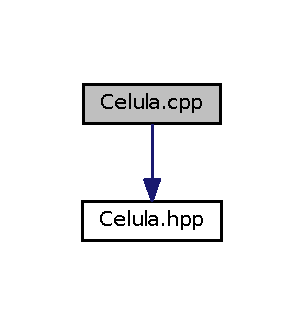
\includegraphics[width=146pt]{_celula_8cpp__incl}
\end{center}
\end{figure}


\subsection{Descripció Detallada}
Implementació de la classe \hyperlink{class_celula}{Celula} de la Pràctica de P\-R\-O2 {\itshape Reproducció al Laboratori}. 

Definició al fitxer \hyperlink{_celula_8cpp_source}{Celula.\-cpp}.


\hypertarget{_celula_8hpp}{\section{Referència del Fitxer Celula.\-hpp}
\label{_celula_8hpp}\index{Celula.\-hpp@{Celula.\-hpp}}
}


Especificació de la classe \hyperlink{class_celula}{Celula} de la Pràctica de P\-R\-O2 {\itshape Reproducció al Laboratori}.  


\subsection*{Classes}
\begin{DoxyCompactItemize}
\item 
class \hyperlink{class_celula}{Celula}
\begin{DoxyCompactList}\small\item\em Representa una cèlula d'un organisme. \end{DoxyCompactList}\end{DoxyCompactItemize}


\subsection{Descripció Detallada}
Especificació de la classe \hyperlink{class_celula}{Celula} de la Pràctica de P\-R\-O2 {\itshape Reproducció al Laboratori}. 

Definició al fitxer \hyperlink{_celula_8hpp_source}{Celula.\-hpp}.


\hypertarget{_organisme_8cpp}{\section{Referència del Fitxer Organisme.\-cpp}
\label{_organisme_8cpp}\index{Organisme.\-cpp@{Organisme.\-cpp}}
}


Implementació de la classe \hyperlink{class_organisme}{Organisme} de la Práctica de P\-R\-O2 {\itshape Reproducció al Laboratori}.  


Inclou el graf de dependències per a Organisme.\-cpp\-:\nopagebreak
\begin{figure}[H]
\begin{center}
\leavevmode
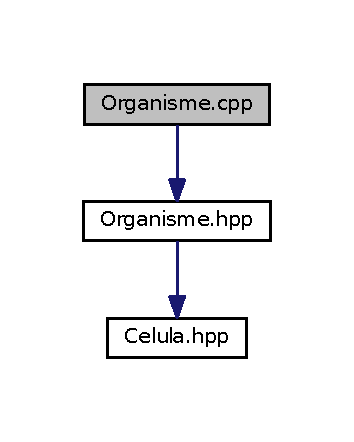
\includegraphics[width=170pt]{_organisme_8cpp__incl}
\end{center}
\end{figure}


\subsection{Descripció Detallada}
Implementació de la classe \hyperlink{class_organisme}{Organisme} de la Práctica de P\-R\-O2 {\itshape Reproducció al Laboratori}. 

Definició al fitxer \hyperlink{_organisme_8cpp_source}{Organisme.\-cpp}.


\hypertarget{_organisme_8hpp}{\section{Referència del Fitxer Organisme.\-hpp}
\label{_organisme_8hpp}\index{Organisme.\-hpp@{Organisme.\-hpp}}
}


Especificació de la classe \hyperlink{class_organisme}{Organisme} de la Pràctica de P\-R\-O2 {\itshape Reproducció al Laboratori}.  


Inclou el graf de dependències per a Organisme.\-hpp\-:\nopagebreak
\begin{figure}[H]
\begin{center}
\leavevmode
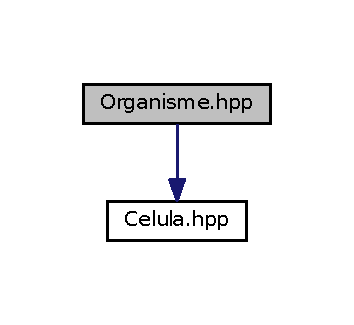
\includegraphics[width=170pt]{_organisme_8hpp__incl}
\end{center}
\end{figure}
\subsection*{Classes}
\begin{DoxyCompactItemize}
\item 
class \hyperlink{class_organisme}{Organisme}
\begin{DoxyCompactList}\small\item\em Representa un organisme de l'experiment. Es caracteritza per tenir un identificador que l'identifica unívocament i un arbre que representa la seva morfologia. \end{DoxyCompactList}\end{DoxyCompactItemize}


\subsection{Descripció Detallada}
Especificació de la classe \hyperlink{class_organisme}{Organisme} de la Pràctica de P\-R\-O2 {\itshape Reproducció al Laboratori}. 

Definició al fitxer \hyperlink{_organisme_8hpp_source}{Organisme.\-hpp}.


\hypertarget{pro2_8cpp}{\section{Referència del Fitxer pro2.\-cpp}
\label{pro2_8cpp}\index{pro2.\-cpp@{pro2.\-cpp}}
}


Programa principal de la Pràctica de P\-R\-O2 {\itshape Reproducció al Laboratori}.  


Inclou el graf de dependències per a pro2.\-cpp\-:\nopagebreak
\begin{figure}[H]
\begin{center}
\leavevmode
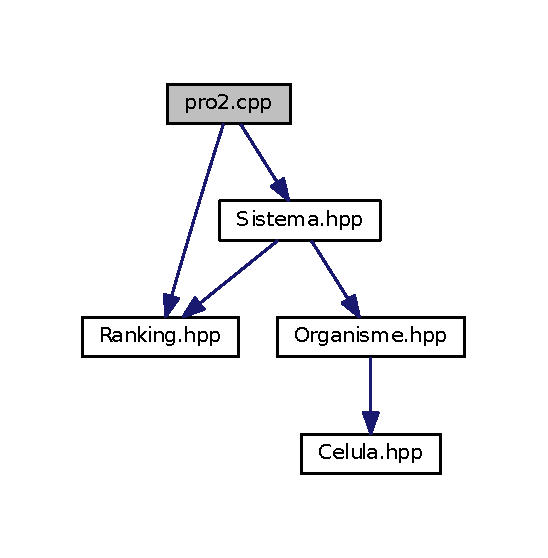
\includegraphics[width=263pt]{pro2_8cpp__incl}
\end{center}
\end{figure}
\subsection*{Funcions}
\begin{DoxyCompactItemize}
\item 
void \hyperlink{pro2_8cpp_af2c9832b3a1f0ccbc1c2c833c71355d0}{aplicar\-Estiraments\-Subcjt} (\hyperlink{class_sistema}{Sistema} \&sis)
\begin{DoxyCompactList}\small\item\em Acció que duu a terme l'opció d'aplicar estiraments a un subconjunt d'organismes de l'experiment. \par
 Aquells organismes llegits pel canal estàndar existents a l'experiment i que no hagin sigut retallats amb anterioritat han patiràn un estirament. \end{DoxyCompactList}\item 
void \hyperlink{pro2_8cpp_aab789a2e4686ea12860641064a37cdc2}{aplicar\-Retallades\-Subcjt} (\hyperlink{class_sistema}{Sistema} \&sis)
\begin{DoxyCompactList}\small\item\em Acció que duu a terme l'opció d'aplicar retallades a un subconjunt d'organismes de l'experiment. \par
 Aquells organismes vius i existents a l'experiment llegits pel canal estàndar d'entrada patiràn una retallada. \end{DoxyCompactList}\item 
void \hyperlink{pro2_8cpp_ad5bcf73bbef300ad36cf3a8f0eb7a824}{consultar\-Subcjt} (\hyperlink{class_sistema}{Sistema} \&sis)
\begin{DoxyCompactList}\small\item\em Acció que duu a terme l'opció de consultar un subconjunt d'organismes de l'experiment. \par
 Aquells organismes llegits pel canal estàndar que existeixin al sistema seràn escrits pel canal estàndar de sortida. \end{DoxyCompactList}\item 
void \hyperlink{pro2_8cpp_a6e100e225d78059dc54d2b086a5d8895}{noti\-Final} (\hyperlink{class_sistema}{Sistema} \&sis, const \hyperlink{class_ranking}{Ranking} \&rank)
\begin{DoxyCompactList}\small\item\em Acció que notifica sobre la causa del final de l'experiment. \par
 S'escriu el nombre d'organismes totals que ha contingut l'experiment i el nombre d'organismes vius en el moment de la fi de l'experiment. \end{DoxyCompactList}\item 
int \hyperlink{pro2_8cpp_ae66f6b31b5ad750f1fe042a706a4e3d4}{main} ()
\begin{DoxyCompactList}\small\item\em Programa principal de la Pràctica de P\-R\-O2 {\itshape Reproducció al Laboratori}. \end{DoxyCompactList}\end{DoxyCompactItemize}
\subsection*{Variables}
\begin{DoxyCompactItemize}
\item 
const int \hyperlink{pro2_8cpp_ab53e564e575059ed07f054f950af7c03}{E\-S\-T\-I\-R\-A\-M\-E\-N\-T} = -\/1
\item 
const int \hyperlink{pro2_8cpp_aa5432982922ef6b26ff9487a76646c94}{R\-E\-T\-A\-L\-L\-A\-D\-A} = -\/2
\item 
const int \hyperlink{pro2_8cpp_a95b449721b616d1608c8c062bda9eb52}{R\-O\-N\-D\-A\-R\-E\-P} = -\/3
\item 
const int \hyperlink{pro2_8cpp_ac56cc8ca3a8ff340d77d045bd895ca0e}{O\-B\-T\-R\-A\-N\-K\-I\-N\-G} = -\/4
\item 
const int \hyperlink{pro2_8cpp_a1c288e39facf9ad6bf7f1d8fe3a40104}{C\-O\-N\-S\-U\-L\-E\-S\-T} = -\/5
\item 
const int \hyperlink{pro2_8cpp_a32c576e3755824cfad8559ab4037310e}{F\-I\-N\-A\-L} = -\/6
\end{DoxyCompactItemize}


\subsection{Descripció Detallada}
Programa principal de la Pràctica de P\-R\-O2 {\itshape Reproducció al Laboratori}. En aquesta pràctica suposem que les dades llegides sempre són correctes, en conseqüència no es fan comprovacions sobre l'entrada. Les opcions a aplicar a l'experiment es representen amb nombres negatius, del -\/1 al -\/6. 

Definició al fitxer \hyperlink{pro2_8cpp_source}{pro2.\-cpp}.



\subsection{Documentació de les Funcions}
\hypertarget{pro2_8cpp_af2c9832b3a1f0ccbc1c2c833c71355d0}{\index{pro2.\-cpp@{pro2.\-cpp}!aplicar\-Estiraments\-Subcjt@{aplicar\-Estiraments\-Subcjt}}
\index{aplicar\-Estiraments\-Subcjt@{aplicar\-Estiraments\-Subcjt}!pro2.cpp@{pro2.\-cpp}}
\subsubsection[{aplicar\-Estiraments\-Subcjt}]{\setlength{\rightskip}{0pt plus 5cm}void aplicar\-Estiraments\-Subcjt (
\begin{DoxyParamCaption}
\item[{{\bf Sistema} \&}]{sis}
\end{DoxyParamCaption}
)}}\label{pro2_8cpp_af2c9832b3a1f0ccbc1c2c833c71355d0}


Acció que duu a terme l'opció d'aplicar estiraments a un subconjunt d'organismes de l'experiment. \par
 Aquells organismes llegits pel canal estàndar existents a l'experiment i que no hagin sigut retallats amb anterioritat han patiràn un estirament. 



Definició a la línia 78 del fitxer pro2.\-cpp.


\begin{DoxyCode}
78                                            \{
79     \textcolor{keywordtype}{int} L = readint();
80 
81     \textcolor{keywordflow}{for} (\textcolor{keywordtype}{int} i = 0; i < L; ++i) \{
82         \textcolor{keywordtype}{int} \textcolor{keywordtype}{id} = readint();
83         \textcolor{comment}{// Només ens cal comprovar que l'organisme és estirable}
84         \textcolor{comment}{// (existeix i no s'ha retallat amb anterioritat) i retallar-lo}
85         \textcolor{comment}{// en cas afirmatiu}
86         \textcolor{keywordflow}{if} (sis.\hyperlink{class_sistema_a3ab5d199d6f7af87c3b00f51702da9dc}{es\_estirable\_org}(\textcolor{keywordtype}{id})) sis.\hyperlink{class_sistema_abe6ae69cefc9adb10b7650635b1f7336}{estirar\_org}(\textcolor{keywordtype}{id});
87     \}
88 \}
\end{DoxyCode}
\hypertarget{pro2_8cpp_aab789a2e4686ea12860641064a37cdc2}{\index{pro2.\-cpp@{pro2.\-cpp}!aplicar\-Retallades\-Subcjt@{aplicar\-Retallades\-Subcjt}}
\index{aplicar\-Retallades\-Subcjt@{aplicar\-Retallades\-Subcjt}!pro2.cpp@{pro2.\-cpp}}
\subsubsection[{aplicar\-Retallades\-Subcjt}]{\setlength{\rightskip}{0pt plus 5cm}void aplicar\-Retallades\-Subcjt (
\begin{DoxyParamCaption}
\item[{{\bf Sistema} \&}]{sis}
\end{DoxyParamCaption}
)}}\label{pro2_8cpp_aab789a2e4686ea12860641064a37cdc2}


Acció que duu a terme l'opció d'aplicar retallades a un subconjunt d'organismes de l'experiment. \par
 Aquells organismes vius i existents a l'experiment llegits pel canal estàndar d'entrada patiràn una retallada. 



Definició a la línia 95 del fitxer pro2.\-cpp.


\begin{DoxyCode}
95                                           \{
96     \textcolor{keywordtype}{int} L = readint();
97 
98     \textcolor{keywordflow}{for} (\textcolor{keywordtype}{int} i = 0; i < L; ++i) \{
99         \textcolor{keywordtype}{int} \textcolor{keywordtype}{id} = readint();
100         \textcolor{comment}{// Només ens cal comprovar que existeix i és viu, i retallar-lo en}
101         \textcolor{comment}{// conseqüència}
102         \textcolor{keywordflow}{if} (sis.\hyperlink{class_sistema_a3eba48be6e01d213f87d9c12c22530fe}{es\_viu\_org}(\textcolor{keywordtype}{id})) sis.\hyperlink{class_sistema_a873e9e89616d383f864191304f804063}{retallar\_org}(\textcolor{keywordtype}{id});
103     \}
104 \}
\end{DoxyCode}
\hypertarget{pro2_8cpp_ad5bcf73bbef300ad36cf3a8f0eb7a824}{\index{pro2.\-cpp@{pro2.\-cpp}!consultar\-Subcjt@{consultar\-Subcjt}}
\index{consultar\-Subcjt@{consultar\-Subcjt}!pro2.cpp@{pro2.\-cpp}}
\subsubsection[{consultar\-Subcjt}]{\setlength{\rightskip}{0pt plus 5cm}void consultar\-Subcjt (
\begin{DoxyParamCaption}
\item[{{\bf Sistema} \&}]{sis}
\end{DoxyParamCaption}
)}}\label{pro2_8cpp_ad5bcf73bbef300ad36cf3a8f0eb7a824}


Acció que duu a terme l'opció de consultar un subconjunt d'organismes de l'experiment. \par
 Aquells organismes llegits pel canal estàndar que existeixin al sistema seràn escrits pel canal estàndar de sortida. 



Definició a la línia 111 del fitxer pro2.\-cpp.


\begin{DoxyCode}
111                                   \{
112     \textcolor{keywordtype}{int} L = readint();
113 
114     cout << \textcolor{stringliteral}{"ORGANISMOS"} << endl;
115     \textcolor{keywordflow}{for} (\textcolor{keywordtype}{int} i = 0; i < L; ++i) \{
116         \textcolor{keywordtype}{int} \textcolor{keywordtype}{id} = readint();
117         \textcolor{comment}{// Comprovem que existeix, i en cas afirmatiu l'escrivim}
118         \textcolor{keywordflow}{if} (sis.\hyperlink{class_sistema_aa56f1fe7fee226ff6624363695ace488}{existeix\_org}(\textcolor{keywordtype}{id})) sis.\hyperlink{class_sistema_ad3028a34f72a19d63a2d126bb4422b5b}{escriure\_org}(\textcolor{keywordtype}{id});
119     \}
120     cout << endl;
121 \}
\end{DoxyCode}
\hypertarget{pro2_8cpp_a6e100e225d78059dc54d2b086a5d8895}{\index{pro2.\-cpp@{pro2.\-cpp}!noti\-Final@{noti\-Final}}
\index{noti\-Final@{noti\-Final}!pro2.cpp@{pro2.\-cpp}}
\subsubsection[{noti\-Final}]{\setlength{\rightskip}{0pt plus 5cm}void noti\-Final (
\begin{DoxyParamCaption}
\item[{{\bf Sistema} \&}]{sis, }
\item[{const {\bf Ranking} \&}]{rank}
\end{DoxyParamCaption}
)}}\label{pro2_8cpp_a6e100e225d78059dc54d2b086a5d8895}


Acció que notifica sobre la causa del final de l'experiment. \par
 S'escriu el nombre d'organismes totals que ha contingut l'experiment i el nombre d'organismes vius en el moment de la fi de l'experiment. 



Definició a la línia 127 del fitxer pro2.\-cpp.


\begin{DoxyCode}
127                                                 \{
128     cout << \textcolor{stringliteral}{"FIN"} << endl << endl
129          << \textcolor{stringliteral}{"Organismos en total : "} << sis.\hyperlink{class_sistema_a084895a86d0230cbb4af0d0041422fe3}{consul\_pob}() << endl
130          << \textcolor{stringliteral}{"Organismos vivos : "} << sis.\hyperlink{class_sistema_a112609f3baf6a0267ce61aab10020418}{consul\_nvius}() << endl << endl;
131 
132     \textcolor{keywordflow}{if} (sis.\hyperlink{class_sistema_adbaf521a9576706bf2212f7ce24d2d0e}{esta\_ple}()) \{
133         cout << \textcolor{stringliteral}{"ORGANISMOS"} << endl;
134         \textcolor{comment}{/* Escrivim els organismes nascuts en l'última ronda
}
135 \textcolor{comment}{           en ordre creixent per identificador. Per la condició
}
136 \textcolor{comment}{           de l'if sabem que si N és la població actual (de fet coincideix
}
137 \textcolor{comment}{           amb la població màxima permesa) i el nombre
}
138 \textcolor{comment}{           d'organismes nascuts a l'última reproducció és R aleshores
}
139 \textcolor{comment}{           tenen per identificadors [N-R+1...N], ja que els identificadors
}
140 \textcolor{comment}{           s'assignen correlativament de menor a major a mesura que neixen
}
141 \textcolor{comment}{           nous organismes */}
142         \textcolor{keywordtype}{int} pob = sis.\hyperlink{class_sistema_a084895a86d0230cbb4af0d0041422fe3}{consul\_pob}();
143         \textcolor{keywordtype}{int} nfillsur = sis.\hyperlink{class_sistema_ad7f3d8c32a3792fec6c4641769c07c04}{consul\_fills\_repr}();
144         \textcolor{keywordflow}{for} (\textcolor{keywordtype}{int} i = pob - nfillsur + 1; i <= pob; ++i) \{
145             sis.\hyperlink{class_sistema_ad3028a34f72a19d63a2d126bb4422b5b}{escriure\_org}(i);
146         \}
147         cout << endl << \textcolor{stringliteral}{"RANKING"} << endl;
148         rank.\hyperlink{class_ranking_aba7a9802d6d3881a19d6fb136b705e07}{escriure\_ranking}(sis.\hyperlink{class_sistema_a084895a86d0230cbb4af0d0041422fe3}{consul\_pob}());
149     \}
150 \}
\end{DoxyCode}
\hypertarget{pro2_8cpp_ae66f6b31b5ad750f1fe042a706a4e3d4}{\index{pro2.\-cpp@{pro2.\-cpp}!main@{main}}
\index{main@{main}!pro2.cpp@{pro2.\-cpp}}
\subsubsection[{main}]{\setlength{\rightskip}{0pt plus 5cm}int main (
\begin{DoxyParamCaption}
{}
\end{DoxyParamCaption}
)}}\label{pro2_8cpp_ae66f6b31b5ad750f1fe042a706a4e3d4}


Programa principal de la Pràctica de P\-R\-O2 {\itshape Reproducció al Laboratori}. 



Definició a la línia 155 del fitxer pro2.\-cpp.


\begin{DoxyCode}
155            \{
156     \textcolor{keywordtype}{int} N = readint(); \textcolor{comment}{// Població inicial de l'experiment}
157     \textcolor{keywordtype}{int} M = readint(); \textcolor{comment}{// Població màxima permesa de l'experiment}
158     \hyperlink{class_sistema}{Sistema} sis(M);
159     sis.llegir\_pob\_ini(N);
160     \hyperlink{class_ranking}{Ranking} rank(M);
161 
162     \textcolor{keywordtype}{int} op; \textcolor{comment}{// Codi d'operació}
163     \textcolor{keywordflow}{while} (sis.consul\_nvius() > 0 and not sis.esta\_ple()
164                                   and cin >> op and op != \hyperlink{pro2_8cpp_a32c576e3755824cfad8559ab4037310e}{FINAL}) \{
165         \textcolor{keywordflow}{switch} (op) \{
166             \textcolor{keywordflow}{case} \hyperlink{pro2_8cpp_ab53e564e575059ed07f054f950af7c03}{ESTIRAMENT}: \hyperlink{pro2_8cpp_af2c9832b3a1f0ccbc1c2c833c71355d0}{aplicarEstiramentsSubcjt}(sis);
167             \textcolor{keywordflow}{break};
168             \textcolor{keywordflow}{case} \hyperlink{pro2_8cpp_aa5432982922ef6b26ff9487a76646c94}{RETALLADA}: \hyperlink{pro2_8cpp_aab789a2e4686ea12860641064a37cdc2}{aplicarRetalladesSubcjt}(sis);
169             \textcolor{keywordflow}{break};
170             \textcolor{keywordflow}{case} \hyperlink{pro2_8cpp_a95b449721b616d1608c8c062bda9eb52}{RONDAREP}:
171                 cout << \textcolor{stringliteral}{"RONDA DE EMPAREJAMIENTOS"} << endl;
172                 sis.aplicar\_ronda\_reproduccio(rank);
173                 cout << \textcolor{stringliteral}{"Nuevos organismos : "} << sis.consul\_fills\_repr()
174                      << endl << endl;
175             \textcolor{keywordflow}{break};
176             \textcolor{keywordflow}{case} \hyperlink{pro2_8cpp_ac56cc8ca3a8ff340d77d045bd895ca0e}{OBTRANKING}:
177                 cout << \textcolor{stringliteral}{"RANKING"} << endl;
178                 rank.escriure\_ranking(sis.consul\_pob());
179             \textcolor{keywordflow}{break};
180             \textcolor{keywordflow}{case} \hyperlink{pro2_8cpp_a1c288e39facf9ad6bf7f1d8fe3a40104}{CONSULEST}: \hyperlink{pro2_8cpp_ad5bcf73bbef300ad36cf3a8f0eb7a824}{consultarSubcjt}(sis);
181             \textcolor{keywordflow}{break};
182         \}
183     \}
184 
185     \hyperlink{pro2_8cpp_a6e100e225d78059dc54d2b086a5d8895}{notiFinal}(sis, rank);
186 \}
\end{DoxyCode}


\subsection{Documentació de les Variables}
\hypertarget{pro2_8cpp_ab53e564e575059ed07f054f950af7c03}{\index{pro2.\-cpp@{pro2.\-cpp}!E\-S\-T\-I\-R\-A\-M\-E\-N\-T@{E\-S\-T\-I\-R\-A\-M\-E\-N\-T}}
\index{E\-S\-T\-I\-R\-A\-M\-E\-N\-T@{E\-S\-T\-I\-R\-A\-M\-E\-N\-T}!pro2.cpp@{pro2.\-cpp}}
\subsubsection[{E\-S\-T\-I\-R\-A\-M\-E\-N\-T}]{\setlength{\rightskip}{0pt plus 5cm}const int E\-S\-T\-I\-R\-A\-M\-E\-N\-T = -\/1}}\label{pro2_8cpp_ab53e564e575059ed07f054f950af7c03}


Definició a la línia 66 del fitxer pro2.\-cpp.

\hypertarget{pro2_8cpp_aa5432982922ef6b26ff9487a76646c94}{\index{pro2.\-cpp@{pro2.\-cpp}!R\-E\-T\-A\-L\-L\-A\-D\-A@{R\-E\-T\-A\-L\-L\-A\-D\-A}}
\index{R\-E\-T\-A\-L\-L\-A\-D\-A@{R\-E\-T\-A\-L\-L\-A\-D\-A}!pro2.cpp@{pro2.\-cpp}}
\subsubsection[{R\-E\-T\-A\-L\-L\-A\-D\-A}]{\setlength{\rightskip}{0pt plus 5cm}const int R\-E\-T\-A\-L\-L\-A\-D\-A = -\/2}}\label{pro2_8cpp_aa5432982922ef6b26ff9487a76646c94}


Definició a la línia 67 del fitxer pro2.\-cpp.

\hypertarget{pro2_8cpp_a95b449721b616d1608c8c062bda9eb52}{\index{pro2.\-cpp@{pro2.\-cpp}!R\-O\-N\-D\-A\-R\-E\-P@{R\-O\-N\-D\-A\-R\-E\-P}}
\index{R\-O\-N\-D\-A\-R\-E\-P@{R\-O\-N\-D\-A\-R\-E\-P}!pro2.cpp@{pro2.\-cpp}}
\subsubsection[{R\-O\-N\-D\-A\-R\-E\-P}]{\setlength{\rightskip}{0pt plus 5cm}const int R\-O\-N\-D\-A\-R\-E\-P = -\/3}}\label{pro2_8cpp_a95b449721b616d1608c8c062bda9eb52}


Definició a la línia 68 del fitxer pro2.\-cpp.

\hypertarget{pro2_8cpp_ac56cc8ca3a8ff340d77d045bd895ca0e}{\index{pro2.\-cpp@{pro2.\-cpp}!O\-B\-T\-R\-A\-N\-K\-I\-N\-G@{O\-B\-T\-R\-A\-N\-K\-I\-N\-G}}
\index{O\-B\-T\-R\-A\-N\-K\-I\-N\-G@{O\-B\-T\-R\-A\-N\-K\-I\-N\-G}!pro2.cpp@{pro2.\-cpp}}
\subsubsection[{O\-B\-T\-R\-A\-N\-K\-I\-N\-G}]{\setlength{\rightskip}{0pt plus 5cm}const int O\-B\-T\-R\-A\-N\-K\-I\-N\-G = -\/4}}\label{pro2_8cpp_ac56cc8ca3a8ff340d77d045bd895ca0e}


Definició a la línia 69 del fitxer pro2.\-cpp.

\hypertarget{pro2_8cpp_a1c288e39facf9ad6bf7f1d8fe3a40104}{\index{pro2.\-cpp@{pro2.\-cpp}!C\-O\-N\-S\-U\-L\-E\-S\-T@{C\-O\-N\-S\-U\-L\-E\-S\-T}}
\index{C\-O\-N\-S\-U\-L\-E\-S\-T@{C\-O\-N\-S\-U\-L\-E\-S\-T}!pro2.cpp@{pro2.\-cpp}}
\subsubsection[{C\-O\-N\-S\-U\-L\-E\-S\-T}]{\setlength{\rightskip}{0pt plus 5cm}const int C\-O\-N\-S\-U\-L\-E\-S\-T = -\/5}}\label{pro2_8cpp_a1c288e39facf9ad6bf7f1d8fe3a40104}


Definició a la línia 70 del fitxer pro2.\-cpp.

\hypertarget{pro2_8cpp_a32c576e3755824cfad8559ab4037310e}{\index{pro2.\-cpp@{pro2.\-cpp}!F\-I\-N\-A\-L@{F\-I\-N\-A\-L}}
\index{F\-I\-N\-A\-L@{F\-I\-N\-A\-L}!pro2.cpp@{pro2.\-cpp}}
\subsubsection[{F\-I\-N\-A\-L}]{\setlength{\rightskip}{0pt plus 5cm}const int F\-I\-N\-A\-L = -\/6}}\label{pro2_8cpp_a32c576e3755824cfad8559ab4037310e}


Definició a la línia 71 del fitxer pro2.\-cpp.


\hypertarget{_ranking_8cpp}{\section{Referència del Fitxer Ranking.\-cpp}
\label{_ranking_8cpp}\index{Ranking.\-cpp@{Ranking.\-cpp}}
}


Implementació de la classe \hyperlink{class_ranking}{Ranking} de la Pràctica de P\-R\-O2 {\itshape Reproducció al Laboratori}.  


Inclou el graf de dependències per a Ranking.\-cpp\-:\nopagebreak
\begin{figure}[H]
\begin{center}
\leavevmode
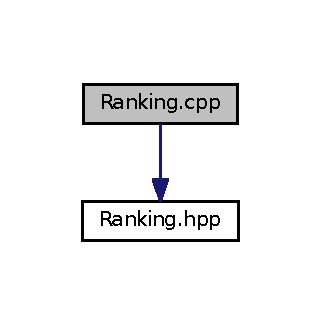
\includegraphics[width=154pt]{_ranking_8cpp__incl}
\end{center}
\end{figure}


\subsection{Descripció Detallada}
Implementació de la classe \hyperlink{class_ranking}{Ranking} de la Pràctica de P\-R\-O2 {\itshape Reproducció al Laboratori}. 

Definició al fitxer \hyperlink{_ranking_8cpp_source}{Ranking.\-cpp}.


\hypertarget{_ranking_8hpp}{\section{Referència del Fitxer Ranking.\-hpp}
\label{_ranking_8hpp}\index{Ranking.\-hpp@{Ranking.\-hpp}}
}


Especificació de la classe \hyperlink{class_ranking}{Ranking} de la Pràctica de P\-R\-O2 {\itshape Reproducció al Laboratori}.  


\subsection*{Classes}
\begin{DoxyCompactItemize}
\item 
class \hyperlink{class_ranking}{Ranking}
\begin{DoxyCompactList}\small\item\em {\bfseries Descripció\-:}\par
 Representa un rànking de reproduccions entre organismes. Es caracteritza per tenir una llista d'enters que representa l'ordre del rànking i un vector amb les llistes d'emparellaments de cada organisme. \end{DoxyCompactList}\item 
struct \hyperlink{struct_ranking_1_1_reproduccio}{Ranking\-::\-Reproduccio}
\begin{DoxyCompactList}\small\item\em Estructura de dades que conté la informació d'una reproducció \end{DoxyCompactList}\item 
struct \hyperlink{struct_ranking_1_1_dades}{Ranking\-::\-Dades}
\begin{DoxyCompactList}\small\item\em Estructura de dades que conté l'informació de les parelles i els fills d'un organisme, a més d'un iterador apuntant a la seva posició en rànking en cas de que s'hagi reproduït. \end{DoxyCompactList}\end{DoxyCompactItemize}


\subsection{Descripció Detallada}
Especificació de la classe \hyperlink{class_ranking}{Ranking} de la Pràctica de P\-R\-O2 {\itshape Reproducció al Laboratori}. 

Definició al fitxer \hyperlink{_ranking_8hpp_source}{Ranking.\-hpp}.


\hypertarget{_sistema_8cpp}{\section{Referència del Fitxer Sistema.\-cpp}
\label{_sistema_8cpp}\index{Sistema.\-cpp@{Sistema.\-cpp}}
}


Implementació de la classe \hyperlink{class_sistema}{Sistema} de la Pràctica de P\-R\-O2 {\itshape Reproducció al Laboratori}.  


Inclou el graf de dependències per a Sistema.\-cpp\-:\nopagebreak
\begin{figure}[H]
\begin{center}
\leavevmode
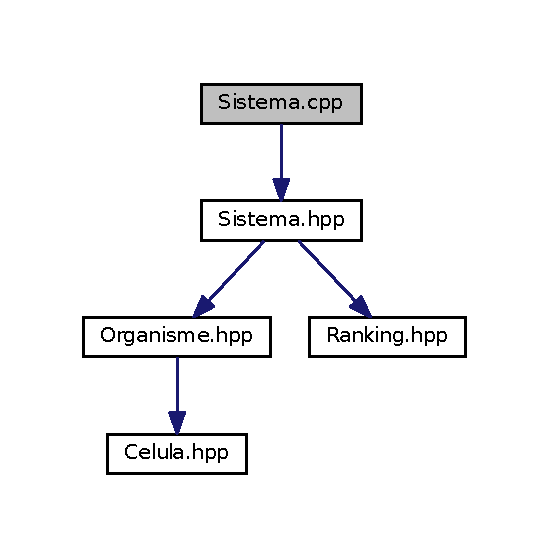
\includegraphics[width=263pt]{_sistema_8cpp__incl}
\end{center}
\end{figure}


\subsection{Descripció Detallada}
Implementació de la classe \hyperlink{class_sistema}{Sistema} de la Pràctica de P\-R\-O2 {\itshape Reproducció al Laboratori}. 

Definició al fitxer \hyperlink{_sistema_8cpp_source}{Sistema.\-cpp}.


\hypertarget{_sistema_8hpp}{\section{Referència del Fitxer Sistema.\-hpp}
\label{_sistema_8hpp}\index{Sistema.\-hpp@{Sistema.\-hpp}}
}


Especificació de la classe \hyperlink{class_sistema}{Sistema} de la Pràctica de P\-R\-O2 {\itshape Reproducció al Laboratori}.  


Inclou el graf de dependències per a Sistema.\-hpp\-:\nopagebreak
\begin{figure}[H]
\begin{center}
\leavevmode
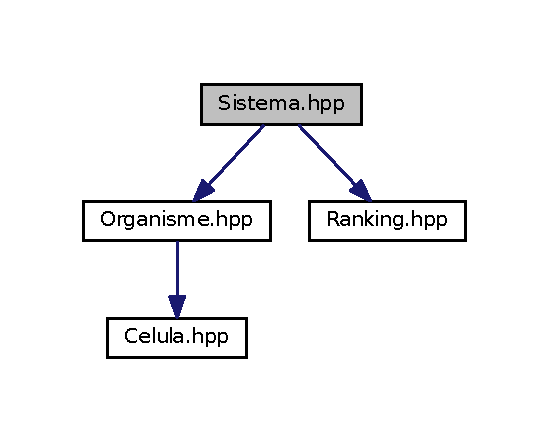
\includegraphics[width=263pt]{_sistema_8hpp__incl}
\end{center}
\end{figure}
\subsection*{Classes}
\begin{DoxyCompactItemize}
\item 
class \hyperlink{class_sistema}{Sistema}
\begin{DoxyCompactList}\small\item\em {\bfseries Descripció} \end{DoxyCompactList}\item 
struct \hyperlink{struct_sistema_1_1_info_emparellaments}{Sistema\-::\-Info\-Emparellaments}
\end{DoxyCompactItemize}


\subsection{Descripció Detallada}
Especificació de la classe \hyperlink{class_sistema}{Sistema} de la Pràctica de P\-R\-O2 {\itshape Reproducció al Laboratori}. 

Definició al fitxer \hyperlink{_sistema_8hpp_source}{Sistema.\-hpp}.


%--- End generated contents ---

% Index
\newpage
\phantomsection
\addcontentsline{toc}{part}{Índex}
\printindex

\end{document}
